\documentclass{book}
% to set font size use
% \documentclass[12pt]{book}

% https://www.overleaf.com/learn/latex/Tables
\usepackage{array}
\newcommand{\dilemmatablewidth}{5.5cm}


\usepackage{graphicx}

% https://www.quora.com/What-font-are-most-books-printed-in
% to set font, use
%\usepackage{ebgaramond}

\usepackage{hyphenat} % http://www.ctex.org/documents/packages/special/hyphenat.pdf

\usepackage{setspace}\onehalfspacing\frenchspacing\flushbottom\sloppy

% https://www.scivision.dev/include-svg-vector-latex/
%\usepackage{svg}
% see https://tex.stackexchange.com/questions/442077/is-it-possible-to-use-svg-images-with-overleaf

% https://tex.stackexchange.com/a/8459/235813
\usepackage[nottoc]{tocbibind}

\usepackage{hyperref}
\hypersetup{
    colorlinks=true,
    linkcolor=blue,
    filecolor=magenta,      
    urlcolor=cyan,
    pdftitle={Overleaf Example},
    pdfpagemode=FullScreen,
    }

% https://en.wikibooks.org/wiki/LaTeX/Glossary says
% "\usepackage{glossaries} and \makeglossaries in your preamble (after \usepackage{hyperref} if present)"

% https://www.overleaf.com/learn/latex/Glossaries
\usepackage[toc]{glossaries}
%\usepackage{glossaries-extra}

\makeglossaries % The command must be before the first glossary entry.

% https://en.wikibooks.org/wiki/LaTeX/Glossary says
% "define any number of \newglossaryentry and \newacronym glossary and acronym entries in your preamble"
% see https://en.wikibooks.org/wiki/LaTeX/Glossary
% and https://www.overleaf.com/learn/latex/Glossaries

\newglossaryentry{organization}{
  name={organization},
  plural={organizations},
  description={an assembly of teams. The name of the concept might be a corporation, an agency, a department, a bureau, or any other aggregation of smaller organizations}
}

\newglossaryentry{culture}{
name={culture},
plural={cultures},
description={norms, expectations around interaction among people}
}

\newglossaryentry{stakeholder}{
name={stakeholder},
plural={stakeholders},
description={a person who cares about the process or the outcome; distinct from a participant}
%descriptionplural={people who cares about the process or the outcome; distinct from participants}
}

\newglossaryentry{participant}{
name={participant},
description={a person who is expected to take action or make contribution}
}

\newglossaryentry{essential bureaucracy}{
name={essential bureaucracy},
text={Essential bureaucracy},
description={the minimum processes and staffing and skills necessary to address the complexity of the problem space}
}

\newglossaryentry{bureaucratic debt}{
name={bureaucratic debt},
plural={bureaucratic debts},
text={Bureaucratic debt},
description={the cost of work need to change a process caused by choosing an easy solution now instead of using a better approach that would take longer}
}

\newglossaryentry{subject}{
    name={subject},
    plural={subjects},
    description={the person experiencing bureaucracy}
}
\newglossaryentry{Prisoner's dilemma}{
    name={Prisoner's dilemma},
    description={Two or more people with incomplete information of a situation will make suboptimal choices compared to someone with perfect knowledge of the situation}
}

\newglossaryentry{thought terminating}{
name={thought terminating},
description={\href{https://en.wikipedia.org/wiki/Thought-terminating_clich\%C3\%A9}{thought terminating statements} initially sound reasonable but, upon reflection and analysis, are incorrect}
}

\newglossaryentry{presence creates priority}{
name={presence creates priority},
description={being physically at a person's desk motivates that person to respond better than calling them or emailing them}
}

% https://graphthinking.blogspot.com/2021/07/bureaucracy-book-outline.html
\newglossaryentry{bureaucrat}{
    name={bureaucrat},
    plural={bureaucrats},
    description={the person who is a member of an organization and is responsible for subjective implementation of policy for the organization. Conventional examples of a bureaucrat role: teacher, police, government employee}
}

\newglossaryentry{simple decision}{
  name={simple decision},
  description={has one correct or beneficial choice and one or more wrong or harmful choices.}
}

% https://tex.stackexchange.com/questions/69567/uppercase-word-in-glossary-lowercase-in-text
\newglossaryentry{bureaucracy}{
    name={bureaucracy},
    plural={bureaucracies},
    text={bureaucracy},
    description={
    An organization of bureaucrats comprises a bureaucracy. A bureaucracy facilitates coordination of stakeholders. 
    Bureaucracy is how large organizations make distributed decisions using distributed knowledge.    \\
    Everything in a bureaucracy is made up by other participants. \\
    Bureaucracy is a macroscopic phenomenon emergent at sufficient scale. The scale is important because there is no longer dependence on individual relationships. \\
    Bureaucracy arises when there is no common objectively quantifiable feedback mechanism for individual participants in the organization.\\
    Bureaucracy is a wicked problem}
}

\newglossaryentry{visible bureaucracy}{
name={visible bureaucracy},
    %name={bureaucracy, visible},
    description={procedures and processes are written down and can be discovered by stakeholders}
}
\newglossaryentry{invisible bureaucracy}{
name={invisible bureaucracy},
    %name={bureaucracy, invisible},
    description={procedures and processes are known to some stakeholders and are conveyed verbally to some of the other stakeholders}
}

\newglossaryentry{process}{
name={process},
plural={processes},
description={a task broken into a specified set of subtask dependencies}
}



\title{How to be an Effective Bureaucrat\\
A Field Guide}
\author{Ben Payne}
\date{\today}

\begin{document}
\pagenumbering{alph} % Fixes problem with glossary links; see https://tex.stackexchange.com/questions/119527/glossary-backlink-points-to-wrong-page

\begin{titlepage}
\maketitle
\thispagestyle{empty}
\end{titlepage}
\newpage

%\thispagestyle{empty}
\frontmatter % the front of the book has roman numerals

%\pagenumbering{gobble}
\thispagestyle{empty}

Copyright \copyright 2022 Ben Payne

\ \\

\href{https://creativecommons.org/licenses/by-nc/4.0/}{Creative Commons Attribution-NonCommercial 4.0 International License}
\clearpage
\thispagestyle{empty}

Thank you to my coworkers. Our interactions me learn how to be a better bureaucrat.%\clearpage
%\pagenumbering{roman}

\chapter*{Foreword}% * excludes from Contents)

% Who this book is for

%If you don't think of yourself as a bureaucrat, I hope to change your mind on this essential topic. 
If you have a negative impression of bureaucracy, I want to convince you that bureaucracy is vital and that you can learn to skillfully navigate bureaucracy.

I see this struggle of bureaucracy as critical to modern society. The challenge of bureaucracy is widespread across a variety of governments in different societies, and bureaucracy is durable -- it has existed for hundreds if not thousands of years. Therefore, tackling the challenge of bureaucracy is exciting for me. I enjoy pondering hard problems and then leveraging insights gained from reflection. Being an effective bureaucrat is important to me because bureaucracy can be a force multiplier beyond what I could accomplish on my own.

% from https://graphthinking.blogspot.com/2021/07/bureaucracy-book-outline.html
This book is for you if you are curious about the complex world we live in, or you are thinking about how to productively contribute to society, or you want impactful employment, or your job is not what you expected. If you're wondering why innovation is hard within a bureaucratic organization, this guidebook is intended to help understand what the challenges are.


% What you should expect reading this book: 
Everyone in modern society is a participant in bureaucracy. The purpose of this book is to decrease the surprise of that experience and better arm you emotionally and intellectually for the toil of being a bureaucrat. With focused reflection and a good guidebook, you can improve your skills as a bureaucrat. 

This book is neither a defense of bureaucracy, nor is it intended to disparage bureaucrats or the system of bureaucracy. Instead, the intent of this book is to serve as a guide to bureaucracy-as-it-is. 

This book does not focus on leadership, managing a team, being a team member, planning, time management, project management, advancing your career, or self-improvement. However, in the process of being a better bureaucrat some lessons may apply in those domains.

This book doesn't address personal stress caused by bureaucracy, how to decrease stress, or how to balance the activities of work and life-outside-work. 

This book doesn't focus on citizens, Congress (state or federal), or competing organizations. 

This book doesn't address discrimination or harassment. This book doesn't address bad coworkers, abusive bosses, psychological defects of individuals, or malicious intent. Issues like lying, bribery, and criminal behavior are not discussed. All these aspects happen whenever people interact; the challenges are not specific to bureaucracy. In this book I assume you are honest, and that other people are honest. Even with this simplifying assumption the complexities of bureaucracy arise. In the context of that benign bureaucracy, guidance on how to be an effective bureaucrat is provided.


% What is the benefit of reading this book?
As a result of reading this book, you will be better able to recognize and navigate complex professional environments, both within your career and outside of work. The perspectives offered in this book can benefit you directly, whether by promotion of title, increase in pay, successful completion of a project, or through decreased stress of understanding how the world operates. Being a more effective bureaucrat can also positive impact the causes you care about and the people you engage with.

If you do not recognize that you are bureaucrat, you won't know what is your own fault, the fault of your coworkers, the fault of management, and what is intrinsic to bureaucracy. 

If you do not recognize that you are bureaucrat, you're less likely to be successful interacting with those around you. The self-recognition of being a bureaucrat matters; how you behave and what you think your responsibilities are depend on how you label yourself.

Even people who are smart (e.g., they know history, they have memorized capital cities, they can do math) can struggle in the face of complex large-scale systems. Thinking about complex large-scale systems is not part of the education curriculum. This book will help you learn about bureaucracy and lead to an increase of your ability to identify patterns and apply relevant techniques.

% there's no avoiding the issue
Everyone is a bureaucrat because there are no alternatives to bureaucracy for a society. Gaining skills in navigating bureaucracy are helpful both for your own happiness and the well-being of a functioning society. 

Hoping that modern technology will eliminate or reduce bureaucracy is not helpful. Automation and computers merely obfuscate processes and make negotiation more challenging. 

Simplifying interactions with other people to ``this is characterized merely as human relations" is an easier perspective compared to considering bureaucracy as a complex system. 
% this is also stated on page 24 of \cite{1991_Wilson}
However, a simplified view either misses emergent phenomena or mischaracterizes the situation. In either case, your effectiveness is harmed.



% my experience
% I wrote this book for a younger version of me.
 When I first started my job in a large organization I recognized differences between the expectations of the education system I had left and the challenges of a professional environment. Over the years I learned from my mistakes by reflecting on my (in)actions and the consequences. This approach has been an expensive education. My mistakes delayed progress and damaged relationships. The motive in this book is to provide generalizations from my experiences which might benefit the reader.


% Caveats

In my reflections and attempting to draw lessons there is a risk of overanalysis. Sometimes a situation is merely happenstance, and sometimes attempting to extract lessons from randomness is folly. Avoiding conjecture about conspiracy and malice is a fuzzy boundary when insufficient information is available. 

My experiences cannot be generalized to every situation. Some of the observations here may be analogous to your context if you squint. 

Nothing in this book is domain specific, nothing is tied to engineering of products, and nothing is applicable solely in science research or policy development. While this material is intended to be timeless and generic, it is culturally specific to the United States of America in the early twenty first century. There are cultural blindspots not addressed in this book because I did not encounter systemic hurdles in my career as financially privileged white male. 

% Source of this content: 
This material is based on personal experience, reading published materials, and anecdotes from other people. No surveys were taken to support the claims made. No double blind experiments were conducted. 

% How the book should be read: 
Reading this book front-to-back is the default option. 
%Chapter~\ref{b_throughout_life} provides context for the lifelong experience of bureaucracy. 
The essentials of bureaucracy described in \S~\ref{fundamentals_of_b} will be familiar to experienced bureaucrats. Each section in Chapter~\ref{b_made_of_humans} is intended to be able to be read stand-alone. The content is intended to spark contemplation. 

\ \\

% as per https://tex.stackexchange.com/q/393238/235813
\begin{flushright}
Ben Payne\\
\today\\
United States of America\\
Earth
\end{flushright}


%\clearpage

\hypertarget{contents}{}
\tableofcontents

\mainmatter % the main part of the book will have standard pages

% https://tex.stackexchange.com/questions/2958/why-is-newpage-ignored-sometimes

\chapter{Introduction to Bureaucracy}
% essentials

  \section{What is Bureaucracy?\label{sec:define_bureaucracy}}

While you may know it when you see or experience bureaucracy, for this book definitions are useful. 

\Gls{bureaucracy} involves creation and execution of \glspl{policy} for managing shared resources. Creating and carrying out policies usually involves multiple people, with each person having specialized roles. Task scalability (how many widgets), complexity (number of steps per widget), or latency (time per widget) drive multiple people to form a hierarchical organization. The organization has control over the disbursement of resources relevant to the society the organization operates within, or administers a policy within that society. Resources managed by the organization are either tangible (e.g., water, air, land) or expertise.  

Bureaucracy is not limited to government. Non-profit organizations, volunteer groups, commercial companies, and even small teams of people can invoke bureaucratic tendencies. The existence of bureaucracy is independent of an organization's purpose. Carrying out someone else's subjectively defined policy will require you to make your own subjective decisions regarding execution and enforcement. 

\ \\

With bureaucracy defined, distinct roles can be identified.
A bureaucracy typically involves a policy creator, a policy enforcer, and the person upon whom policy is inflicted. In the context of government, the policy creator can be either a politician or a bureaucrat. 

An organization comprised of bureaucrats is a \gls{bureaucracy}. The protagonist within a bureaucracy is the \gls{bureaucrat} -- the person who is a member of an organization and is responsible for subjective implementation of policy for the organization. The person that a bureaucrat's decisions are inflicted on a \gls{subject}.  Depending on context, a subject may be a student (when the bureaucrat is a teacher) or a subject may be a citizen if the bureaucrat is a police officer or government official. Sometimes a bureaucrat's decisions are inflicted on other bureaucrats-as-subjects, such as when a Chief of Police creates guidelines for police in their district, or when a senior diplomat sets policy for embassy employees. 


A \gls{bureaucrat} is a person subjectively interpreting policies on behalf of an organization and has discretionary enforcement. The bureaucrat's purpose is to facilitate coordination of stakeholders by applying specialized knowledge. 

Let's break that down piece-by-piece. First, ``subjective interpretation'' means there is a person making a decision about how to do something. The subjectivity arises from different reasons one person might choose an option over a competing option.  A \gls{policy} is a set of actions in a given circumstance. An \gls{organization} is the collection of people for who the policy is made. Discretionary enforcement means the person is choosing how to apply the policy in the specific circumstances. Facilitating coordination means bureaucracy is about getting multiple people (or sometimes a person at different instances in time) to work together. The stakeholders are people who care about the application of the action in each circumstance.  That's still pretty dense, so the rest of the book is spent expanding the nuances and implications of this definition.

Bureaucracy is neither good nor bad. Bureaucracy is not tied to politics, nor is bureaucracy specific to an institution (corporations, governments, academia). The definition of bureaucracy used in this book is independent of government. Bureaucracy is not defined to be efficient; nor does it have to be inefficient. Bureaucracy is not restricted to paperwork, record keeping, quantification, or gathering metrics. Nothing in this definition involves paperwork or an office building. Definitions that limit the concept of bureaucracy to specific contexts result in a decreased ability to describe complex large-scale human organizations. 

Bureaucracy is about delegation of control, communication, decision making, coordination, and processes. Bureaucracy relies on negotiation. 


A critical aspect of bureaucracy is that everything is made up, specifically by other humans. The consequence is that everything is negotiable. You (in the role of either a subject or a bureaucrat) need to know both who to negotiate with and how to negotiate the desired changes. My claim that bureaucracy is made up is in contrast to actual rules -- the mathematical physics that describe nature. Everything in your environment is either naturally occurring macroscopic emergent phenomena (e.g., chemistry, biology) or humans making up labels and norms. Distinguishing the two is critical to knowing what you can change and what you have to operate within. 

Bureaucracy arises when there is no common, objectively quantifiable feedback mechanism for individual participants in the organization. This aspect is why governments, schools, and prisons are characterized as bureaucratic. The military doesn't rank soldiers by ``number of enemies killed'' and is bureaucratic. Even profit-driven commercial organizations are bureaucratic when the impacts of individual employees are not coupled to the metrics of profit. 

Profit-based feedback makes some roles in a business context slightly more predictable and understandable. Even in that situation there are trade-offs like externalization of costs and long-term profit versus short-term profit. 

The concept of bureaucracy is most visible for complex recurring situations involving many people and the control of a shared resource. The apparent friction of bureaucratic processes can be lower when there are only a few people involved (``I'm just talking to my collaborator" or ``I'm just buying groceries from a clerk at the store'' or ``I'm using a website for a government service''), but there is a continuous gradient to more obvious instances of bureaucracy. Bureucratic tendencies are observable at the small scale; they typically get ignored or called something else.

Bureaucracy arises when management of a shared resource is necessary; that resource can be external to the organization or internal to the organization. Examples of external resources include mail delivery for \href{https://en.wikipedia.org/wiki/United_States_Postal_Service}{USPS}, public safety for \href{https://en.wikipedia.org/wiki/Federal_Bureau_of_Investigation}{FBI}, and the environment for \href{https://en.wikipedia.org/wiki/United_States_Environmental_Protection_Agency}{EPA}. The focus of this book is on internal resources. Resources internal to a bureaucratic organization include intangibles like attention, skill, expertise. Metrics like time, money, and staffing are proxy measures for the central intangible resources.



Bureaucracy is a system for distributed knowledge and distributed decision making. That is in contrast to easier-to-understand concepts like centralized knowledge and centralized decision making. A government run by dictatorship is easy to conceptualize compared to democracies because there is a central character around which a narrative can be formed. Similarly, stories about the \href{https://en.wikipedia.org/wiki/Chief_executive_officer}{CEO} of a company are much easier than capturing the thousands of interactions conducted by the many employees of that company. The vast majority of the work an organization does is coordinated and carried out by people other than the CEO. Linear story-telling with a small number of protagonists does not map well to the complexities of bureaucracy. 


\newpage % section
  \section{Bureaucrat's view of their Organization\label{sec:alternative_views_from_within}}

Bureaucracy as I have defined it in \S\ref{sec:define_bureaucracy} is not the only way that bureaucrats perceive their environment. Bureaucrats typically focus on themselves, their work, their subjects, their coworkers, their superiors, and their subordinates. The motives of an individual bureaucrat for any given activity varies. The variance is even more complicated a request costs additional work and there's no deadline and there's no reward. What is your incentive? Emotional approval? Relationship building? Social approval?

\ \\

The perspectives below are archetypal for bureaucrats who don't consider bureaucracy as defined in \S\ref{sec:define_bureaucracy}; an individual's perspective might be a mixture of these views.

\ \\
\textbf{As a bureaucrat, what matters is what I can accomplish with my skills and the resources I have access to.} \\
\textit{Assessment}: This person is task oriented. Results are what matters. The intricacies of bureaucracy are a distraction to getting the work done. 
% https://graphthinking.blogspot.com/2015/05/a-method-for-herding-cats.html
Communication  for the purpose of coordination is a distraction from work of the individual. 
This bureaucrat may have the perception that if they initiate formation of a community, they will be blamed when things go wrong.
The emotional reward for this person is accomplishment of the task. This person is likely to say to their manager, ``Tell me what I need to do to be successful" rather than identify collaborations.

\ \\
\textbf{As a bureaucrat, what matters is how I feel.} \\
\textit{Assessment}: Your feelings are real. They have consequence, in that your emotions impact motivation and enthusiasm. However, a feelings-centric perspective may not be productive for you or your team or the organization. Being effective means compromise and some people may not get everything they wanted. Balancing those competing needs is challenging.

\ \\ 
\textbf{What matters is how others feel.}\\
\textit{Assessment}: Depending on the emotional state of those around you is unhealthy and can be unproductive. Working for the happiness or satisfaction of other people is risky -- they may not know what's best, or they may not have your interests in mind.

\ \\
\textbf{What matters are my immediate coworkers.}\\
This perspective can be positive (I collaborate with those around me) or negative (I am in competition with those around me).
In this scenario everything beyond the local scope is personified or ignored.  \\
\textit{Assessment}: Your do relationships matter. However, they are not all that matters. Missing from this view is the ability to explain what is happening outside the immediately observable realm. 

\ \\

Just because you are a bureaucrat doesn't mean you have a well-informed understanding of bureaucracy. Regardless of their perspective, a bureaucrat certainly experiences the difficulties of operating within an organization. The bureaucrat rationalizes to themselves why things don't work in an org with stories like
\begin{itemize}
\item other people are lazy / don't want to work
\item other people are inexperienced
\item other people don't care
\end{itemize}
without realizing other people may characterize the bureaucrat with those same stories. 
  \section{Models of Bureaucracy\label{sec:models-of-bureaucracy}}

Coming up with a holistic theory of bureaucracy is desirable but difficult. Bureaucracy exists in every society, so having an explanatory theory would help identify what is critical and what is not essential. Having a theory of bureaucracy could help identify what should be improved and what should be discarded. An expectation for the existence of a theory stems from the repeated independent creation of bureaucracy in diverse societies in different time periods. 

Characterizing bureaucracy is difficult because organizations comprised of unique humans are aware of attempts to be characterized and respond to stories told about bureaucracy; see the \href{https://en.wikipedia.org/wiki/Hawthorne_effect}{Hawthorne effect}. As soon as a claim about bureaucracy-as-a-concept is made, then an individual can respond to that claim by behaving in an opposing manner. Worse still for the theory, bureaucrats can coordinate to provide counterexamples. 

In the following section I outline a few ways of modeling bureaucracy for the purpose of pointing out the shortcomings of each model. The relevance to the practicing bureaucrat of familiarity with these models is so that you know the boundaries of each model. Awareness of the limitations of each model enables you to know when the model is an applicable story and when the model is not explanatory. 

\subsection{Bureaucracy as a Machine}

\textit{Narrative}: Bureaucracy is a machine that has throughput and latency and dependencies and mechanisms. Bureaucrats are cogs in that machine.\\
\textit{Why this feels true}: Bureaucracy can be complicated and feel mechanical with standardization, top-down dictates, and interlocking processes. There is a risk of \href{https://en.wikipedia.org/wiki/Deindividuation}{deindividuation} for bureaucrats. \\
\textit{What this is missing}: Perceiving yourself as a cog in the wheel implies a loss of agency. This is a \href{https://en.wikipedia.org/wiki/Self-fulfilling_prophecy}{self-fulfilling prophecy} -- if you think you don't have agency, then you stop having agency. 

% TODO: any citations for this view?

\subsection{Bureaucracy as an Economic model}

\textit{Narrative 1}: A Bureaucracy is a collection of individual rational actors. \\
% https://graphthinking.blogspot.com/2019/05/cooperation-and-competition.html
Individual bureaucrats cooperate or compete to promote their own self-interests.
The culture of an organization is a result of individual self-interests of each bureaucrat.
Individuals make decisions that promote their own self-interests.

This view is hard for me to distinguish from a marketplace. 

\ \\

\textit{Narrative 2}: A Bureaucracy is comprised of competing special-interest groups. \\
The observation of \href{https://en.wikipedia.org/wiki/Public_choice}{Public Choice theory} is that a concentrated minority that stands to gain a disproportionate benefit will act in their own self-interest. In a generic bureaucratic organization it is not clear which team would be more concentrated than any other team, and what the disproportionate benefit might be. There is a concentrated minority at the top of any hierarchy, and the top of the hierarchy does act in their own self-interest, though this is not particular to bureaucracy.

Bureaucratic organizations may have specific teams with access to disproportionate benefits, but this book focuses on generic bureaucratic features. (Effective bureaucrats are all alike; every bureaucrat is ineffective in their own way?\footnote{A modified version of the first sentence of Leo Tolstoy's novel ``Anna Karenina.''})

% TODO: any citations for this view?

\ \\

\textit{Narrative 3}: A Bureaucracy as a subcategory of a Firm. \\
% https://graphthinking.blogspot.com/2017/09/market-friction-and-bureaucratic.html
Firms exist in a market because negotiating contracts and prices for every interaction is burdensome. 
% https://www.kellogg.northwestern.edu/faculty/hubbard/htm/research/ec174/lectures/3coase.htm
A bureaucracy could be considered as a type of firm that specializes at the organizational level in policy administration or resource management. 

%Doesn't address small vs large companies, and doesn't distinguish between profit-oriented and non-profit and government. 


\subsection{Bureaucracy as Emergent phenomenon}

\textit{Narrative}: There is a universality to bureaucracy in both the diversity of scenarios and persistence across time that hints at \href{https://en.wikipedia.org/wiki/Emergence}{emergence}. Bureaucracy as a macroscopic phenomenon is emergent at when there are a sufficient number of people. The size of the organization is important because there is no longer dependence on individual relationships (beyond \href{https://en.wikipedia.org/wiki/Dunbar\%27s_number}{Dunbar's number}). There are people in the organization that you don't know and for which there is no personal accountability. An organization is subdivided into teams recursively until there is local person-to-person accountability.  The underlying behaviors that enable emergence are bilateral interactions among humans and a lack of feedback mechanisms. 

At the scale of individual bureaucrats, every person is playing by different rules and has different objectives and everything is changing -- both the individuals and the conditions. 
Above the threshold for emergence of bureaucracy there is scale-free behavior. The same patterns are observable at large organizations and extremely large organizations. A bureaucrat in one organization recognizes patterns of professional life experienced by bureaucrats at another organization. The local mechanisms bureaucrats employ to enable distributed decisions using distributed knowledge include meetings, processes, and communications. 

The choices faced by an individual bureaucrat are not independent of the choices made by other bureaucrats in their environment. There is a \href{https://en.wikipedia.org/wiki/Flocking_(behavior)}{flocking behavior} of my choices are informed by the choices of those around me. Unlike flocking of birds, the adjacency metric for bureaucrats is not necessarily spatial distance.


The relevance of claiming bureaucracy is emergent is that there is behavior occurring at the macroscopic scale; knowing that individual motives and actions of every player at the microscopic level is not relevant. Treating organizations as complex and adaptive systems gives insight on how to work within the dynamic environment \cite{2011_Eisenhardt}.


A colloquial interpretation of emergent behavior from complex phenomena is treating the system as an entity -- personification.\marginpar{[Tag] Fallacy} When an organization is assigned behaviors \cite{2002_Gall}, it is useful to remember that the organization is comprised of individual bureaucrats. 


% https://www.preposterousuniverse.com/podcast/2021/10/11/168-anil-seth-on-emergence-information-and-consciousness/
More formally, there are distinct categories of emergence \cite{2002_Bedau}. Nominal emergence names the phenomena of a thing being distinct from its constituents: a circle is emergent from a collection of points; a pile of sand emerges from grains of sand. Merely putting many bureaucrats in a room is insufficient to create bureaucracy; there are additional aspects necessary to bureaucracy. 

Weak emergence occurs when there are phenomena that are independent of the underlying interactions. For example, \href{https://en.wikipedia.org/wiki/Glider_(Conway\%27s_Life)}{gliders} in \href{https://en.wikipedia.org/wiki/Conway\%27s_Game_of_Life}{Conway's Game of Life}.
Weak emergence is measurable using \href{https://en.wikipedia.org/wiki/Granger_causality}{Granger causality} or, equivalently\footnote{\href{https://arxiv.org/abs/0910.4514}{https://arxiv.org/abs/0910.4514}}, \href{https://en.wikipedia.org/wiki/Transfer_entropy}{transfer entropy} (information theory). I don't know how to apply these measures to bureaucratic organizations. 

\textit{What this model is missing}: The problem with treating an organization as an entity is that apparent behavior is counter-intuitive. Breaking the organization into individual people with motives helps clarify the cause of the behavior. 
%This merely improve the post hoc rationalization. 

In practice, bureaucracy is worse than emergent because the rules can be altered or ignored by the stakeholders. Bureaucracy is a \href{https://en.wikipedia.org/wiki/Wicked_problem}{wicked problem} which resists mathematical models. 

\subsection{Bureaucracy in Game Theory}
\textit{Narrative}: Bureaucracy can be understood as one or more games played by bureaucrats. 

\textit{What this model is missing}: Bureaucracy defined as distributed knowledge and distributed decision making does not fit cleanly into the game theory categories of being either cooperative or \href{https://en.wikipedia.org/wiki/Non-cooperative_game_theory}{competitive} -- in practice there are elements of both. 

% not relevant: \href{https://en.wikipedia.org/wiki/Coordination_game}{coordination game}

Another frame for interactions within a bureaucracy is to consider a variety of games. This view is similar to market conditions. Which game is applicable depends on the specifics of the situation. 

%Bureaucracy is self-modifying. 
Bureaucracy is in constant flux due to external conditions, externally imposed constraints, staff turn-over, internal dilemmas, disagreements of individuals. 




\subsection{Bureaucracy as Evolutionary Outcome}


\textit{Narrative 1}: Biological, Genetic -- Individual level. \\
Biological arguments for gene-based bureaucracy. Zebra fish and hyenas have a gene is for dominance. \footnote{``Society, demography and genetic structure in the spotted hyena'' (2012); doi:10.1111/j.1365-294X.2011.05240.x}

%Breeding animals for aggressiveness?

\textit{What this model is missing}: Non-human animals make subjective decisions and 

\ \\

\textit{Narrative 2}: Biological, Genetic -- Group selection. \\
Hierarchy (\S\ref{sec:hierarchy_of_roles}) is not unique to humans. Primates form into social hierarchies based on dominance over a shared resources like mates and food.

\textit{What this model is missing}: a gene for bureaucracy. A genetic model does not explain what specific behaviors an individual bureaucrat can take to be more effective. 

\ \\

\textit{Narrative 3}: \href{https://en.wikipedia.org/wiki/Memetics}{Memetic} -- bureaucracy as method for coordination is a better idea than nepotism or religion. \\
\textit{What this model is missing}: bureaucracy persists along with nepotism and religion, and bureaucracy occurs within religion. 

\subsection{Bureaucracy as Product-focused Narrative}
\textit{Narrative}: Ignore the bureaucrats and instead focus on how a product progresses through processes.\\
\textit{Example}: \href{https://www.youtube.com/watch?v=OgVKvqTItto}{School House Rock's I'm Just A Bill}\\
\textit{What this model is missing}: Ignoring bureaucrats involved in processes simplifies the narrative (the product is the protagonist). 

\subsection{Bureaucracy as Subject-focused Narrative}
\textit{Narrative}: Ignore the bureaucrats and instead focus on the person subjected to bureaucracy. \\
\textit{Why this feels true}: The person experiencing bureaucracy as a subject is confused by ``why isn't this easier?''  \\
\textit{What this model is missing}: History of the processes (legacy) and protection against malicious subjects and protection against malicious bureaucrats. 


\subsection{Bureaucracy as Psychological Phenomenon}

\textit{Narrative}: Bureaucracy as a pure power struggle. Or the interplay of individual psychosis. \\
%Are you doing what's best for you, the group you're in, or everyone?
%Altruistic or reciprocal? Retaliation.
%The answer changes time the time and situation of situation and person to person.

%Just a mixture of pathologies?

%\href{https://en.wikipedia.org/wiki/Spiral_of_silence}{Spiral of silence}
% and
%\href{https://en.wikipedia.org/wiki/Social_proof}{social proof}

Organizations are composed of individuals with personalities, and inefficiency is attributable to a mashing together of distinct individuals with conflicting desires.
While this is true, it isn't complete. \\
\textit{What this model is missing}: Personality-focused narrative neglects the history of processes (legacy) and protection against malicious subjects and protection against malicious bureaucrats. Analysis that stops at personalities misses emergent phenomena. Analysis that stops at personalities of individuals typically explains larger scale phenomena using personification of teams and organizations. 

\ \\

Each of the above models has shortcomings. Knowing why each model is not a complete description helps you avoid the trap of thinking only in terms of a single model. 

The rest of this book ignores these partial characterizations of bureaucracy. 
Rather than take the external (\href{https://en.wikipedia.org/wiki/Emic_and_etic}{emic}) view of bureaucracy, this book takes the internal (etic) perspective of a bureaucrat operating within an organization. 
The description of bureaucracy in this book is to contextualize the advice for how to be an effective bureaucrat. \newpage % section

  \section{Fundamentals of Bureaucracy\label{fundamentals_of_b}}
  
  This section provides terminology and definition for a bureaucratic lens. Specifically bureaucracy is defined and labels for roles in bureaucracy are named. Structure in organizations is often characterized by hierarchy, and that hierarchy is described by an ``organization chart.'' Lastly, meetings and written communication are the way in which consensus among bureaucrats is established.

    % define the core concepts 
    \subsection{Hierarchy of Roles\label{sec:hierarchy_of_roles}}

Ideally sufficient depth and breath for decision making would be embodied in one person. That might not be possible in every situation. One way to resolve this is to identify distinct scopes of responsibility and then assign different members of an organization separate scopes for decision making. Within a decision making scope there may be more work than one person can handle, so a team is formed. That team may have some members focused on tactical work and other members focused on strategy and coordination. Hierarchy within an organization is the formalization of separate decision-making scopes and associated specialization. 

Partitioning knowledge and decision making enables complexity beyond what one person can accomplish and causes friction among members. An expert reporting to a manager knows things the manager does not, and the manager may have context that the expert lacks. Both bureaucrats (the expert and the manager) need to convey their respective nuance and seek out the holistic view.

A hierarchical organization with partitioned knowledge introduces a challenge: the order in which you share information with others matters. Your choices for who to first describe an idea to are your peers, your management, and your subordinates. \marginpar{[Tag] Trilemma} The people subordinate to you know more about the topic and are exposed to the consequences. Giving them a chance to vet the idea results in a more robust idea and validates their value in organization. Sharing your idea with management first allows your superiors to provide context you might not be aware off. Starting the conversation with your peers first indicates you value the relationship and decrease the risk of overlapping work.

\ \\

Although I've included hierarchy in the section on Fundamentals of Bureaucracy, I don't mean to imply that hierarchy is a required feature of bureaucracy. Hierarchies of bureaucrats are a common \href{https://en.wikipedia.org/wiki/Organizational_structure}{organizational structure} and therefore worthy studying even if not essential to bureaucracy. The relevance of understanding hierarchy is to identify recurring behavior and patterns to leverage.
Organizations of bureaucrats can intentionally work against hierarchy, but the amount of effort needed to enable alternatives implies that hierarchy is a natural approach.

The benefits of formal hierarchy include improved capacity for the number of policy decision made, enabling consistency of decisions, and leveraging specialization of knowledge. 
Hierarchical decision making has costs: higher latency, inconsistency among bureaucrats, waste due to inefficiency, and many others described in \S\ref{sec:unavoidable_hazards}. As another example of harm, hierarchy enables strategic ignorance. Bureaucrats in positions of power can deny having knowledge of improper activity. 
\footnote{L.~McGoey, ``The Unknowers: How Strategic Ignorance Rules the World" (2019)
% review: https://www.tandfonline.com/doi/abs/10.1080/19460171.2020.1768422?journalCode=rcps20
and 
L.~McGoey, ``The logic of strategic ignorance" (2012). DOI 
10.1111/j.1468-4446.2012.01424.x
}


The structure of an organization is dynamic, but at each point in time an organization typically has a defined set of roles. Each role is distinguished by different scopes of decision authority. 




Roles in an organization are defined by the boundaries of responsibility. The purpose of a role is to minimize conflict and reduce redundancy, allowing control. Clear responsibility enables effective bureaucracy. 


A conventional characterization of an organization's hierarchy involves two criteria: the depth and breadth of the org chart.
The more people a supervisor oversees, the flatter the organization -- that's the breadth of the organization. See the Valve handbook \cite{2012_Valve} and Joreen's essay \cite{1972_Joreen} for contrasting views on the shape of an organization's hierarchy. Depth of the hierarchy is how many layers there are.

A more practical view of an organization's hierarchy also involves two criteria. The two choices in how a hierarchy is shaped are 
1) how many people a supervisor oversees and 
2) how many supervisors a person has. 
Though you might naively expect that an employee has one boss, but that is \href{https://en.wikipedia.org/wiki/Matrix_management}{not a requirement}. A supervisor for a given topic may have many people reporting to them, and a bureaucrat with multiple roles may report to more than one supervisor.

\ \\

Acting as part of a group means ceding part of your autonomy. Hierarchy is an additional layer of ceding responsibility and adding expectations about relationships.
The consequence of hierarchy in an organization means that as a member of the bureaucracy you do not have full autonomy -- otherwise you would not be a member of the hierarchy. At the same time you are not under strict control of the organization -- you still have some subjective decision making authority as a bureaucrat.

The person at the top of the hierarchy does not know everything. The person at the top of the hierarchy does not have input on every decision made in the organization. Some autonomy is retained by all members of the bureaucracy.

Independent of the defined roles and designated titles in an organization's hierarchy, there are a set of implicit roles and a separate social hierarchy of informal influencers and decision makers. Informal influencers in a bureaucracy usually have long relationships with the decision maker or relevant credentials or both. The credentials can be formal (e.g., a \href{https://en.wikipedia.org/wiki/Doctor_of_Philosophy}{PhD}) or informal (demonstrated success on a project). In either case, the decision maker is relying on another person's expertise. 

Another set of informal relations within an organization is mentors and mentees. These relations allow mentors to transmit institutional knowledge to mentees, and allows people in senior positions to access the novice perspective. 


\ \\

One consequence of hierarchy is a sense of fear felt by people who report to other people. This fear stems from the loss of control (less autonomy) that leaves the person feeling disempowered. 

For example, consider the following relationship. A person, Sue, is perceived to have power over another person, Amy, because Amy gave up some control to Sue. Amy not having control triggers the feeling of fear in Amy, regardless of how Sue behaves. 

If Sue is aware of the potential for this emotional experience, Sue can compensate for Amy's fear by being friendly and receptive towards Amy. Alternatively Sue may exploit or rely on the fear felt by subordinates. 


% Active bystander when the person doing wrong is in a position of authority
% PACT (Probe, Alert, Challenge, Take Action)
% https://mobile.twitter.com/GeorgetownABLE/status/1408498438203969541


% Mintzberg's Coordination Mechanisms
% https://www.youtube.com/watch?v=IZET8VjSifQ


    \subsection{Organizational chart as a guide and a lie}

An \href{https://en.wikipedia.org/wiki/Organizational_chart}{organizational chart} (hereafter ``org chart'') identifies roles and the relations among roles. An org chart is at best a snapshot in time, and more often aspirational than descriptive. In spite of possible deficiencies, an org chart helps outsiders and newcomers understand the scope of responsibilities and interactions.\footnote{The organization chart hasn't always existed. The \href{https://en.wikipedia.org/wiki/George_Holt_Henshaw\#First_organization_chart}{first known org chart} was created in the 1850s.}

Org charts are a lie in the sense that undocumented relationships can matter more than the roles. Org charts fail to capture the informal roles that facilitate progress in any organization. 

Org charts foster a lie by creating sense power dynamics based on visual orientation. For more on this issue see \S~\ref{org-chart-orientation}.

    \section{Not many Options for Organizations}
% https://graphthinking.blogspot.com/2021/07/patterns-anti-patterns-in-bureaucracy.html

Organizations comprised of bureaucrats have fewer options than individual bureaucrats. The choices an individual bureaucrat faces are described in the section on dilemmas, \S\ref{sec:dilemma_trilemma}. In comparison, the choices faced in the design of an organization are
\begin{itemize}
    \item flatness of organizational hierarchy
    \item number of supervisors per employee
    \item teams: create a new team, merge existing teams, dissolve a team
    \item processes: hiring, promotion (pay or title), professional training, firing
\end{itemize}
In a government bureaucracy, pay and financial incentives are typically set outside the organization.

The organization may have policies and processes regarding hiring, promotion, training, and firing, but the decision may not be made by the top-level management. 

\subsubsection{Not many options for Teams}

Team managers decide who gets hired and who gets promoted and who goes to what training and who gets fired.

Among teams, interactions are either lateral (sideways) or parent-child (top-down) or child-parent (bottom-up) \cite{2014_Jorgensen}.

The child-parent bottom-up upward communication is either inadequate (too few updates, or not enough information, or insufficient context), relevant, or excessive. Finding the balance depends on the presenter knowing the individual audience members so that a tailored message is provided, and adapting to the specifics of the situation. A weekly or monthly report to multiple superiors is inadequate. 
% tips on managing up: 
% https://svpg.com/managing-up/

The parent-child downward communication either is inadequate (no direction), provides actionable vision, or micromanagement. 

For lateral interactions among teams, the tension between cooperation and competition manifest in struggles over
\begin{itemize}
    \item money
    \item staffing
    \item prestige
    \item products (output)
    \item resources (inputs)
    \begin{itemize}
        \item access to or control of data
        \item technology resources
        \item hardware
        \item floor space
        \item expertise
    \end{itemize}
\end{itemize}



    \subsection{Meetings for Coordination\label{sec:meetings-for-coordination}}
In an organization comprised of more than one person, meetings are necessary for facilitating coordination. The coordination accomplished by a meeting can be explicit (verbal or written), or it can be indirect through signaling (who attended the meeting, when the meeting was held, where the meeting was held, how much notice was provided). 

No everyone understands that meetings are a vital aspect of coordination in a bureaucracy. The following sequence of scenarios illustrate the thinking some bureaucrats apply. (If you're already convinced of the value of meetings, see tips on improvement in \S~\ref{well-run_meeting}.)


\ \\

% https://graphthinking.blogspot.com/2021/07/thought-terminating-concepts-in.html
\textit{Anti-meeting view}: No plan or coordination needed; I just do what you tell me. With this approach, either I will be successful because I worked hard on what my supervisor directed, or I will fail because I was directed to do the wrong thing by my supervisor.\\
\textit{Potential response 1 by the supervisor}: I think you're smart, and I think you're capable of shaping your career. Let's work as a team to improve your effectiveness. \\
\textit{Potential response 2 by the supervisor}: Is that how you want your career to go? Do you desire autonomy and creativity?

\ \\

\textit{Anti-meeting view}: No point in making a plan or coordinating because everything changes so frequently. \\
\textit{Potential response by the supervisor}: But the effort has an end goal, right?\\
\textit{Anti-meeting view}:  Yes, so then the plan is to get from where we are now to that end goal. Coordinate as necessary. \\
\textit{Potential response by the supervisor}: And there are no intermediary steps? Milestones?
Is it better to have no plans and just put up fires reactively, or to have a plan that is subject to change? To wait for a need for coordination?

\ \\

\textit{Anti-meeting view}: What is a plan anyways?\\
\textit{Potential response by the supervisor}: There is value in creating a goal, enumerating tasks that would support the goal, identifying the dependencies among the sub-tasks, and time-binning the dependencies with defined milestones and deliverables. That is my definition of a plan. And having that is more useful than merely reacting.

\ \\

\textit{Anti-meeting view}: Who's plan? Who's relationships? I don't need to come up with that plan, the supervisor already has a plan. Just tell me what the plan is.\\
\textit{Potential response by the supervisor}: That's not as effective as coming up with independent plans and then resolving the differences. There's value in resolving the differences, Even though that will cost time and frustration and displace time to implement.


    \section{Written Communication}

Report, emails, memos


action with the deadline

responsiveness % this isn't essential, just common
    \subsection{Decision making in a bureaucracy}

Sometimes events unfold organically without necessarily decisions being made. Whether because the decision makers are not informed, or there is an intentional neglect.

One way to avoid the appearance of subjective decision making on policy is to frame the process as "data driven." 
% https://graphthinking.blogspot.com/2018/06/data-driven-decisions-versus-data.html


% https://graphthinking.blogspot.com/2019/01/political-decisions-versus-science.html
A decision is political when the basis is historical relationships, maintenance or creation of a relationship, or to enable future relationships.
In contrast, a quantitative decision basis is based on measurements.


What appears from the outside as ``organizational inertia'' is internal delay of decision making and the delay of dissemination. 
Delay comes from
\begin{itemize}
    \item It takes time for each decision maker to gather information, arrive at a decision, modify processes, disseminate their selection, justify their selection. 
    \item forcing a continuous variable into a discrete set of choices. Typically the number of choices is small. Discrete choices for a continuous variable is a loss of effectiveness.
    % https://dynomight.net/teaching/
    \item processes designed to account for cheaters and people with malicious intent, whether that means a malicious bureaucrat or malicious subject. 
\item Analysis paralysis, due to {insufficient information, too much information, which framing is unclear}
\item When other people who are needed to carry out the action push back, either in disagreement or seeking clarification. The fact that the organization is not profit driven is important because the justification for the action isn't quantitatively obvious. Therefore there's a higher burden for communication.
\end{itemize}


A \gls{simple decision} has one correct or beneficial choice and one or more wrong or harmful choices. The work of decision making is to gather information that identifies which is the correct or beneficial choice and select that option.

Best case scenario is one person making a well-informed simple decision that has immediate consequence and the consequence is to the decision maker. Example from elementary formal education: arithmetic math problems, multiple choice quizzes, spelling tests, memorization tests. 

A complex decision may have many choices, and there are might not be a best option. Then a \href{https://en.wikipedia.org/wiki/Pareto_front}{Pareto frontier} might exist where trade-offs can be made. 

As an example of a complex decision made by one person with immediate consequence and direct relevance to the decision maker, suppose you want to purchase a car. You car about only two aspects: fuel efficiency and cost. 

\begin{figure}[ht]
    \centering
    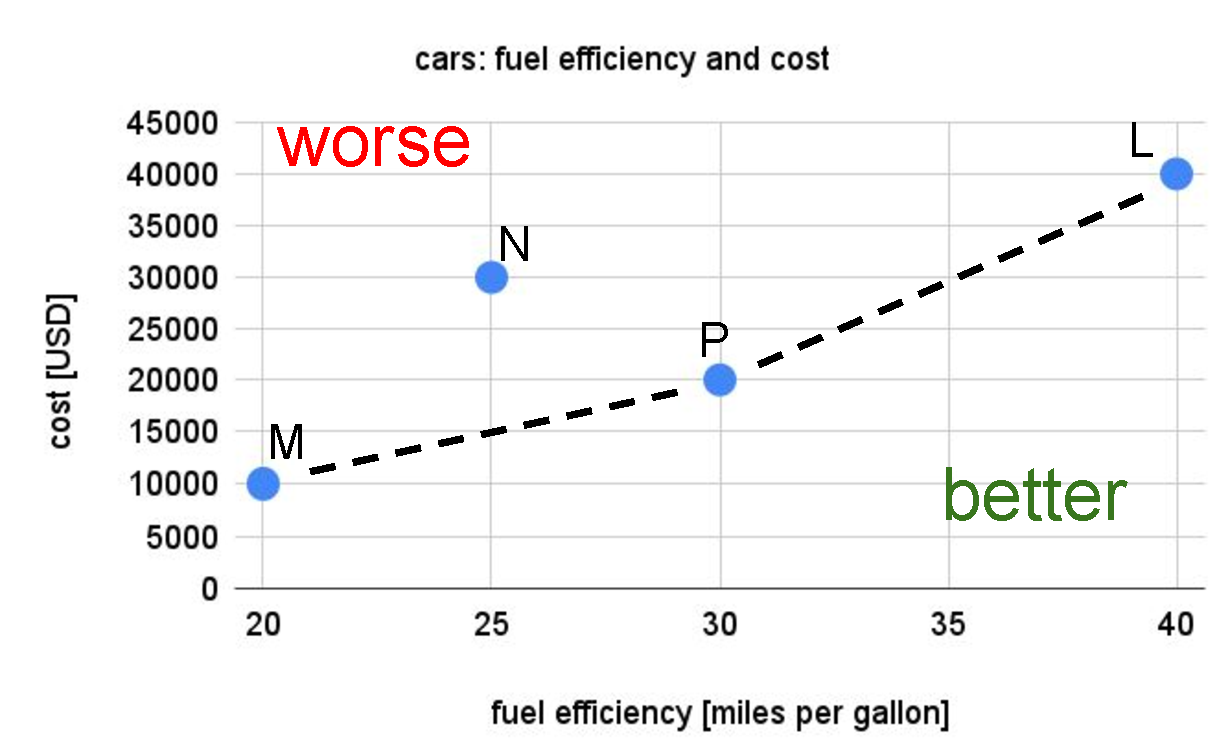
\includegraphics[width=1\textwidth]{images/pareto_frontier_car_options.pdf}
    \caption{Four cars, L, M, N, and P. Goal is to spend less money and get better fuel efficiency. Choices not on the frontier should be avoided, but that doesn't yield a single result.}
    \label{fig:pareto_frontier_cars}
\end{figure}

A common pareto frontier in generic decision making is the trade-off between speed, accuracy, and cost. 

Pareto frontier analysis works well when there are many options relative to the number of variables being optimized for. Does not account for relative importance of different variables.

The assessment does not work as well when there are few choices relative to the number of variables. For example, suppose there are 10 choices of car and I want high fuel efficiency, high cargo capacity, maximum number of passengers, stylish, low cost, low maintenance, good durability, and high resale value. might need to assign weights to each of these factors. 

A typical decision is ill-informed, has diffuse consequences, delayed impact, and does not affect the decision maker. 

Even afterwards a decision can be difficult to evaluate for correctness because there are multiple stakeholders.

In bureaucratic processes there is rarely a formal assessment of options. 
Decisions are rarely recorded. 

Decision making by bureaucrats can be informal or formal, consensus-based or solo. 

Most decisions made by bureaucrats do not have hard deadlines. Instead, there are trade-offs in timing. Sooner is better, but delaying allows for more information gathering for a better informed decision.




Decision makers face options and have the goal of identifying a beneficial outcome (for which stakeholders?). The goal is to reduce uncertainty among options. Two ways to reduce uncertainty: gather more information (takes time), or push the decision down the chain (to people with narrower view). 

If a bureaucrat is going to rely on expert consultation, the decision maker needs to be confident the expert is not of straying outside their area of expertise. For example, I don't rely on a botanist with many published papers to tell me how to change the oil in my car. 

When getting input for a decision, is the expert providing a factual summary, a predictive assessment, or a value judgement? 

There are many ways to gather evidence. 
Role of measurement and modeling. 
Form an opinion, look for evidence to back the outcome.
Instead of measurement, most people rely on history (if they are aware of it), or what is best for their career, or how to accumulate more power, or what someone else says to do.  

    \subsection{Feedback loops}

When there is a lack of feedback from customers/users, then someone has to decide.


when there are multiple competing objectives among different stakeholders in a zero sum use of resources, how to determine what's best? Typically there are feedback loops to guide progress. When feedback loops are weak or not present, then the most powerful stakeholder (which is distinct from the biggest or loudest) will dominate. 

\subsubsection{Special interest groups}

when there is a benefit to a small group and the cost is to a larger group

\subsubsection{Spending taxpayer dollars}

Suppose I earn \$100,000 and the tax rate is 30\%. Then my tax money sent to the government is \$30,000.

"In 2021, the [US] government collected \$4.05 trillion in revenue."
\footnote{source: Government Revenue | U.S. Treasury Data Lab}

My taxes of \$30,000 is
30000/4050000000000 = 0.00000074\%

When I do not maximize the effectiveness of \$1,000,000 of government money, of that misallocated money \$0.0074, or about one penny, was taxes I paid. The feedback loop is weak.

Federal pay is limited to about \$220,000\footnote{https://en.wikipedia.org/wiki/Executive\_Schedule}, so that raises the feedback to 2 pennies.

The lack of feedback allows waste to go unfelt. There's no immediate consequence.
Waste is indistinguishable from not enough funding or insufficient skills 




Feedback loop:
\begin{center}
\begin{figure}[ht]
    \centering
    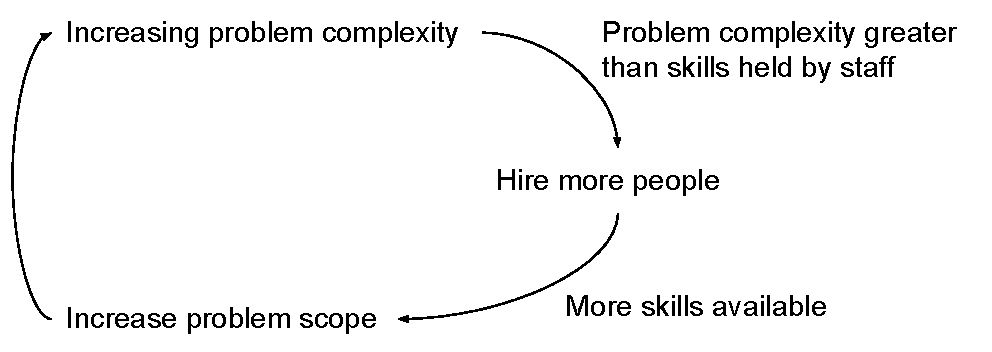
\includegraphics[width=0.8\textwidth]{images/feedback_loop_complexity_and_staffing}
    \caption{Complexity requires more staffing; having more staff means more skills are available; under-utilized staff skills make room for more scope; more scope adds to complexity.}
    \label{fig:complexity_and_staff_growth}
\end{figure}
\end{center}


% source: 
% https://graphthinking.blogspot.com/2019/07/altering-feedback-loops-to-change.html
Bob parks his car in a parking garage every day. The parking garage owner charges \$20 per day for people to park their car.

Bob recently found that one of the exit gates for the parking garage is broken. If Bob uses that gate to leave the parking garage, the gate does not function and Bob cannot exit. Then Bob has to call the parking gate operator to request an exception (which is granted) and Bob can then exit that gate, avoiding the \$20/day charge.

This action (go to broken gate, request exception, avoid charge) has been repeated for a long time (months). Bob's motive is to avoid the \$20 parking charge; the cost is a mere phone call and a minor delay. This cheating behavior harms the parking garage owner's income. However, the parking gate operator, serving as intermediary, insulates the parking garage owner from the interaction with the cheater. The cheating behavior is small enough that the parking garage owner may not notice.


\subsubsection{Meeting time compared to theft}
% https://graphthinking.blogspot.com/2021/02/organizations-value-things-more-than.html

Source: \cite{1995_Grove}.

In large organizations, there can be significant bureaucracy associated with even small purchases. A multi-step review process may be incurred for a \$2000 acquisition.

Another measurement of value is that if an employee were to steal even \$200 worth of materials, the organization would likely punish that employee.


Those metrics apply to tangible goods, but not to people's time. Consider a meeting of 10 people and each person's cost is \$200 per hour. A wasted meeting is not unusual and certainly would not incur bureaucratic review processes. The cost to the organization is fiscally the same -- \$2000. Similarly, consider an employee who is late and causes a loss of productivity. Merely depriving the organization of \$200 worth of time is not punished in the same way theft is.

In fact, organizations default to meetings (even recurring meetings) rather than not meet. And being late to a meeting is accepted. 

We can debate the differences between theft of materials and theft of time. The financial argument is clear. 
 % subsection
  \newpage
  \section{History of Bureaucracy}

I'm mostly going to skip history and merely cite other scholarly references


https://en.wikipedia.org/wiki/Bureaucracy\newpage % section
  \section{Scope of bureaucracy}
  %\begin{flushright}
  %Back to the \hyperlink{contents}{Table of Contents}
  %\end{flushright}
    \subsection{Who is a bureaucrat?}

A cashier in a gas station is a bureaucrat. The ``policy'' might simply be ``take money from customer in exchange for items and gas,'' but the subjective application of that policy leaves a lot of room for the cashier to shape the customer's experience. Does the cashier greet the customer when the customer enters the store? Does the cashier look at the customer to acknowledge the customer? Smile? How quickly does the cashier engage the customer? Minor nuances that are left to the cashier in the execution of the store policy means there is room for subjective application of the policy. 

% examples of bureaucrats
A bank teller, a loan officer, and a bank's \href{https://en.wikipedia.org/wiki/Technical_support}{technical support} are all bureaucrats. Each person subjectively enforces policies on behalf of the organization. The directness of financial impact for the person varies among these roles. Of these three roles, the loan officer's interactions with bank customers provides the clearest feedback on profit. The loan officer doesn't act alone though -- the customer's interactions with tellers and the bank's technical systems also matter to the customer's decision. 


This same discretionary application of policy applies to commercial bureaucrats like sandwich makers, car salespeople, oil well drillers, grocery clerks, retail clerks, and plumbers. Public school teachers, state and federal police, military members, tax collectors, and other state workers are government bureaucrats. 


% bureaucracy is not limited to white collard office workers
Factory line workers subjectively apply policies. Enforcement of quality standards is the most obvious area. Pacing of work is a negotiation with management that directly impacts productivity and profits.

Structured environments like sports featuring well defined rules do not eliminate bureaucracy. Teammates use subjective policies on who to work with and how to best leverage their strengths and exploit the opponent's weaknesses. The policies are set in part by the coach. Referees make subjective determinations about rules.

Sometimes bureaucrats do not work directly with customers or citizens or products. Then the bureaucratic process is inflicted on fellow bureaucrats. In this scenario, a bureaucrat is subjectively applying a policy to other bureaucrats. 

Identifying yourself as a bureaucrat matters, both to the employee and to the business. The risk of not self-identifying as a bureaucrat is that you won't grasp how much control you have in implementing and enforcing policy. If you think of yourself as having to blindly follow rules, you will harm the people you are applying the rules to and you will harm the business/institution you are applying the rules for. Adapting policies to circumstances is the value of having judgement capacity. 

In a similar sense from the consumer/citizen perspective, if you don't think you are interacting with a bureaucracy, you won't perceive the opportunity to negotiate.  If you view rules as fixed and inflexible, you will harm your ability to make progress. If a rule was made by a human, then that rule is flexible. Who made the rule? Who enforces the rule? If you can talk to them, could they be convinced to make a modification or an exception?

If you don't think about a bureaucratic framing, you might think the store clerk is enforcing a policy because they don't like you. Assigning personality conflict as the cause might lead to a different conversation with their manager (the person who created the policy). 

If you don't think of yourself as a bureaucrat, you'll behave differently in your job. The paradigm of ``just tell me what to do'' is the default (learned in school) and you won't know how to engage with coworkers/bosses since they are not friends. You will be less likely to understand how to leverage the organization and identify collective wisdom. Thinking from the perspective of a bureaucrat explains why evangelizing within your organization is relevant. 
%You'll see your coworkers as competitors for promotion.

% https://graphthinking.blogspot.com/2020/10/impact-of-self-identifying-as-not.html
If you think of yourself as merely a cog in a machine, you are less likely to notice that you exert influence in the process and you are less likely to recognize the autonomy available to you. 
If you think ``I have a real job (e.g., nurse, cashier, teacher), therefore I'm not a bureaucrat", you are less likely to recognize the subjective power you have in interactions with the public.
If you think, ``I'm at the bottom of my organization's hierarchy, therefore I do not have power", you are less likely to notice the autonomy when it is available.

If you don't think of yourself as part of a bureaucratic process, you'll behave differently in interactions with bureaucrats.  You won't perceive opportunities to negotiate because the processes seem fixed instead of subjective. 
You won't recognize motives and incentives of bureaucrats, so their activities will seem incomprehensible.


 % subsection
    \subsection{Number of People in a Bureaucracy}

Although bureaucracy can be present for one person, and bureaucracy is often apparent on teams (e.g., 3 to 20 people), this book focuses on the situation of multiple teams comprising an organization. This might be a few hundred people (above \href{https://en.wikipedia.org/wiki/Dunbar's_number}{Dunbar's number}) up to millions of people. 
Examples of companies that employ more than a million people\footnote{see \href{https://en.wikipedia.org/wiki/List_of_largest_employers}{Wikipedia's list of largest employers}} include Walmart, Amazon, and McDonald's. Size isn't a requirement for bureaucracy. Small companies with a few people incur bureaucracy because of the need for coordination of subjective policies governing shared resources. Non-profit organizations encounter bureaucracy. 
Bureaucracy emerges in small organizations, has patterns that are scale invariant, and is generic across sectors. The complexity of the tasks may be different, but the same scale-independent patterns can emerge because of a common factor: human behavior.

% https://graphthinking.blogspot.com/2017/05/population-sizes-needed-to-support.html
The size of bureaucracy scales with the complexity of the problem. For example, if participants in a society only used hand tools they could make themselves, then there is little need for bureaucracy. Mining and producing small amounts of metal is feasible for an individual, though the relevance of specialization becomes clearer. A society large enough to support the technology of writing (beyond the use of clay tablets) seems to coincide with the bureaucratic need for writing. Getting to technology like the telegraph and radio requires a society that supports complex processes and specialization -- key aspects of bureaucratic systems. While decreasing bureaucracy is certainly feasible, it's not clear how to maintain the current technological sophistication. 


In addition to essential task complexity, the size of bureaucracy depends on accidental factors like how old the bureaucracy is, how big the community being supported is, and how diverse the community is.


 % subsection
    \subsection{Why does bureaucracy exist? Can't we just do the work?}

Monarchies and dictatorships the rely on a single decider. A simpler model to understand, but difficult to handle all the edge cases for large society. 

Political representatives are an easier to understand concept because it's just one person acting in that behalf of other people.
In contrast emergent behavior of bureaucracy is more difficult to understand. TODO: why not make the entire system out of politicians?

TODO: thought experiment: 
What if everybody in a bureaucracy were the same?
What if everybody in a bureaucracy had a different opinion?


The short answer is that bureaucracy is a response to the complexity of a problem being solved. To see why that is, let's start simple and then increase the complexity. 

The minimal scenario to start from is to imagine a single person working on a single task that does not last long (a few minutes), is relatively easy (cognitively and physically and emotionally), and does not recur. In that situation, building consensus is irrelevant and no process is required. 

Most of what you do occurs outside those limits and thus incurs some concept of \gls{process} (breaking a task into subtasks). Staying with the one-person constraint, a complex task can benefit from being broken into subtasks. Sometimes the order of the subtasks matters, so we need to track the dependencies. A recurring multi-step process with documentation is starting to have features of bureaucracy, but lacks the need for consensus. 

If one person lacks the skills relevant to a multi-step process, they may engage another person to help. The interaction may be informal (anarchy) or formalized in a contract (\href{https://en.wikipedia.org/wiki/Libertarianism}{libertarian}). If the parties working on the task fail to reach consensus, what is the recourse? Options include physical violence, threats, or involving a third party (e.g., a court with lawyers and judges). 


The bureaucrat's identity is subsumed into service for the organization they are part of. At the same time, bureaucracy enables the bureaucrat to amplify their presence by being part of a larger organization. A bureaucrat can accomplish more as part of an organization than by working alone. Sometimes the cost of being part of the organization exceeds the force multiplier of working together. 

% https://graphthinking.blogspot.com/2021/09/why-is-everything-so-hard-in-large.html

What if we completely avoided bureaucracy? That question is better worded by replacing ``bureaucracy" with ``coordination of stakeholders". If you avoid coordination of stakeholders, you either are constrained to only work on tasks that involve one person, or you get is random (uncoordinated) interactions. 

What if we minimized bureaucracy? Again, try replacing ``bureaucracy" in that question with ``coordination of stakeholders". The goal of ``minimizing coordination" probably isn't the real objective. To be more precise, a specific objective might be ``minimize time spent executing the task" (which takes a lot of coordination prior to the task execution) or ``minimize the level of distraction to stakeholders" (chunk the coordination time). Another strategy for minimizing bureaucracy is to reduce the number of stakeholders involved. For a given task complexity, this means having smarter people who have more skills. 

\begin{figure}
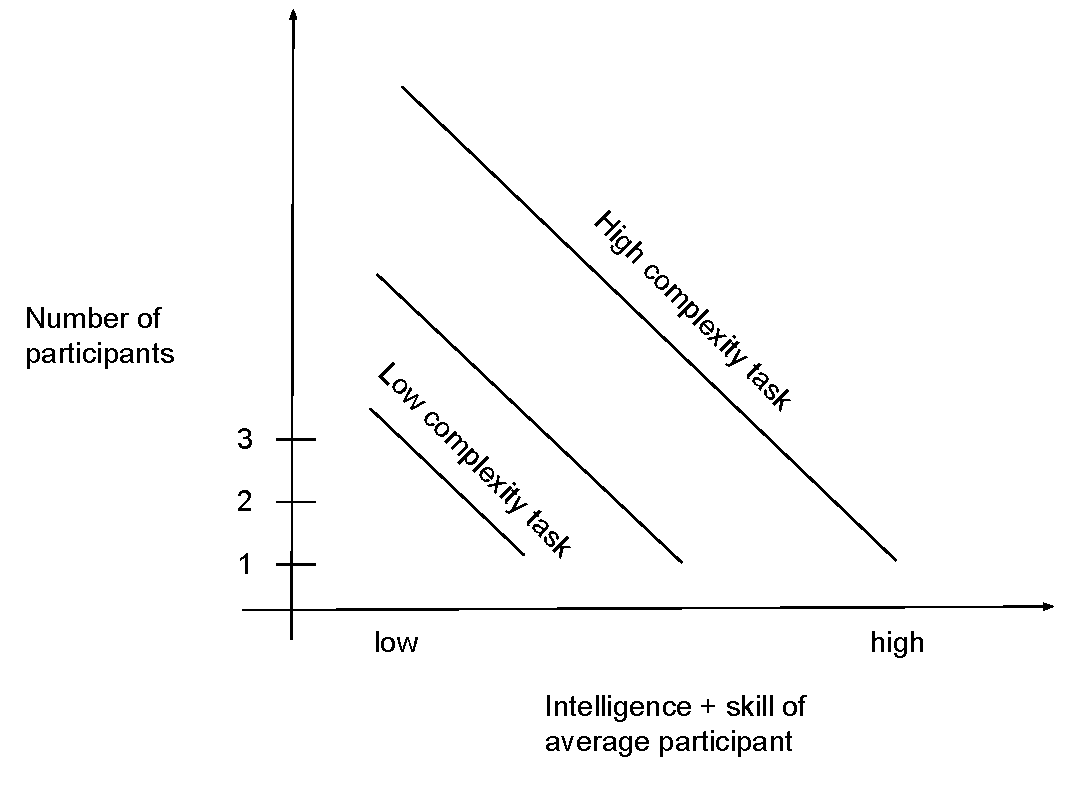
\includegraphics[width=0.8\textwidth]{images/people-per-task-for-skill-level.pdf}
\caption{Three levels of task complexity are shown. As task complexity increases, the size of the team needs to grow. The growth may be less if the team members are brilliant. Those brilliant people cost more and there are fewer of them available.}
\end{figure}
 % subsection
    \subsection{Why is bureaucracy so hard?}

When a person has a positive experience engaging with bureaucracy, positive attribution is made to the people involved. Or ease of a solution makes the bureaucracy less visible and the solution seems obvious. 

When a person has a negative experience with bureaucracy, complaints are about the incompetence of the people involved, or the incomprehensibleness of the system. Don't these bureaucrats know how to do their job? Why isn't the solution obvious? Why does this system not work for me?

many nuances not visible to external perspective
\begin{itemize}
    \item organization politics (personalities, resources, prioritization)
\item lack of unified voice
\item legacy policies to overcome/change/be consistent with
\end{itemize}




  %\section{From Startup to Bureaucracy}

In a novel domain, people show up in order: nerds (who find the domain intrinsically interesting prior to value being available), then commoners (who don't find intrinsic value in the domain), then jackasses (who look to exploit infrastructure, resources, and people). 


\chapter{Bureaucracy in general}
  \section{Each Phase of Life involves Bureaucracy}
In each person's life there are standard milestones: birth, education, work, death. 
The relationships in each phase are distinct.
Each of these milestones and phases involves bureaucracy. Each phase is a different experience of bureaucracy because the bureaucratic roles change.

\subsection{Bureaucracy of Birth\label{sec:bureacracy-of-birth}}
Your birth was marked by getting a name, registering with the state, and initiating medical records. These tasks were administered by bureaucrats on your behalf. The bureaucrats included the hospital staff, and you were the subject of the bureaucracy. You had no autonomy or decision making authority. 

\subsection{Bureaucracy in early childhood\label{sec:bureaucracy-early-childhood}}
Prior to starting education, the bureaucracy of early childhood is inflicted primarily by family members setting and carrying out policies. The organization of bureaucrats is the family. Other community members or caretakers may also be involved to carry out the polices of taking care of you. Your decision making authority was extremely limited. 

\subsection{Bureaucrats at School\label{sec:bureaucracy-of-school}}
Once you started the education process, new bureaucrats got involved.  The community of bureaucrats could be a public school, a private school, or homeschooling. In any of those cases, the frontline bureaucrat is the teacher. You don't have responsibility for making policy that other people follow; you are still the subject of bureaucracy.


The expectations of each phase of school (high school, undergraduate, graduate school) are distinct, and they are different from working in a large organization. Your autonomy increases throughout the duration of school. %, and your ability to make policy that effects others grows. 
Your family and teachers are the bureaucrats. You start building informal organizations of friends, and you start to explore policies around social bonding.

Schooling sets a pattern that most students will fall into for the rest of their lives. You were handed a textbook and told to solve a set of problems. You have the autonomy to do more than what is required. You can find other textbooks that match your interests or are written from a different view. 

You get to choose the book you want, even if you don't get to choose the topic you are going to be evaluated on. You don't even need to pick just one reference book -- you can pick lots of books and figure out which author style best fits you. You can also choose the level of difficulty -- very basic and beginner level, or more advanced (depending on where you are, rather than where a class in school is supposed to be).

You can discover how you learn best. This extra effort requires self-reflection: How did you learn? What worked best? What didn't work, and why not? What did you learn? What do you wish you had learned?

Another pattern that schooling relies on is single choice decisions where there is only one right answer. Examples include math problems and multiple choice tests. Schooling tends to avoid setting up dilemmas or paradoxes for students. Academic problems in the education process are designed to be independent of the people involved or the history of the situation. 


% https://graphthinking.blogspot.com/2013/02/all-little-things.html
%Where you sit in the classroom matters. Being in the front means you will be exposed to fewer distractions, more likely to pay attention.


% https://graphthinking.blogspot.com/2012/09/how-to-not-be-average.html
%How were you taught? Did you have any input on the method?
%Who taught? Did you like them? Were they friendly, knowledgeable, and approachable?


% https://graphthinking.blogspot.com/2012/09/how-to-not-be-average.html
%What resources are available now for you to learn from? Do you like learning?
%you have the freedom to pursue what ever intellectual endeavors you want.


% https://graphthinking.blogspot.com/2011/09/which-skills-are-useful-after.html

% did not prepare me for addressing challenges at work. 
In my schooling I learned how to approach technical issues and develop solutions. That problem-solution paradigm neglects crucial steps of discovering the problem, isolating the challenge, identifying stakeholders, learning the history of the challenge, and negotiating with stakeholders before attempting to address the challenge. 

My schooling led me to emphasize academics over socializing. When I transitioned to professional work, I realized that social skills and political savvy useful when attempting to change organizations and policies. 

Unlike academic problems that rely on and evaluate my answers, working in a bureaucratic organization the challenges are ill-defined, there's no known solution, and the problem is sufficiently complex that I have to collaborate.

% https://graphthinking.blogspot.com/2018/07/the-difference-between-problems-at.html


%\subsection{undergrad vs graduate}
% education process roles and expectations vary over time

%college, graduate school: friends, teachers, advisors



\subsection{Military Service Bureaucracy\label{bureaucracy-of-military}}
Less than 0.5\% of the United States population serves in the military\footnote{source: \href{https://www.cfr.org/backgrounder/demographics-us-military}{Council on Foreign Relations}}. For those who do serve, the military's rigid hierarchy and defined protocols is a distinct experience compared to school or work. The transition from military to civilian life can present a dissonance for service members used to the chain of command and clearly defined orders. 

\subsection{Working in a bureaucratic organization\label{sec:bureaucracy-of-work}}
Within the employment phase, there are pairs start and end events which may apply: hiring or getting hired; firing, getting fired, or quitting. 

employment: managers above you, peer employees, people you manage are all members of an organization. 


You encounter shared resources at work: bathrooms, conference rooms, kitchen areas with fridges and microwaves, storage areas. 

Bathroom example: the bathroom smells sometimes so I'm a nice person and I bring a scented air freshener. Unbeknownst to me, that triggers an asthma or allergic reaction for my coworkers. Now a policy gets created so this mistake doesn't happen again. Signs are posted. 


\subsection{Healthcare and Death\label{sec:bureaucracy-of-death}}
Doctors and nurses are bureaucrats; you are the subject; the hospital or clinic is the organization. 


Toilet paper at the hospital
If you go to a hospital, use the bathroom, and find there is no toilet paper, that would indicate a deficiency.
Someone didn't refill the toilet paper. Since the person who normally refills toilet paper wasn't also a user, they aren't directly impacted by the lack of toilet paper.
So someone needs to have a routine of checking bathrooms for toilet paper availability. Money spent checking to toilet paper is money not spent on the primary mission of the hospital.
Minimizing checking is important, so a feedback mechanism is instituted -- a phone number to text regarding bathroom status at the hospital.



Death can invoke both the medical system and the government. 



\ \\

All of these roles and relationship involve subjectively administered policies within an organization. The point of recognizing the role of bureaucrats is to help you identify what is negotiable. 


 \clearpage
  \section{Avoiding Bureaucracy is Nearly Impossible}

The only situation where bureaucracy might not exist is if you live completely on your own, with no interaction with other people. That means completely disengaging from society. Even then, personal routines are a self-imposed form of bureaucracy, with the roles of policy maker, bureaucrat, and subject collapsed to a single person -- you.

Self-sufficiency and autonomy are attractive alternatives bureaucracy. The way participants in modern society strive for self-sufficiency is by denying their dependence on modern society. That's a relabeling of selfishness which feels better. 

For the rest of us who operate as members of a society, bureaucracy is necessary for our rights. We prove our name by cooperating with other people, and our name helps us claim our citizenship. That's a subjective policy that \glspl{stakeholder} in society agree to. 



The specific way a society is constructed (democratic, authoritarian, dictatorship, anarchy) is irrelevant -- bureaucracy is still present. Even the libertarian view of relying on contract enforcement implies some amount of bureaucracy (e.g., forums for resolving contract disputes like a court system). 


Not all bureaucracy is due to the state, nor is bureaucracy confined to companies. Parenting involves coming up with situation-specific requirements for children, with the organization being the family as mentioned in \S\ref{sec:bureaucracy-early-childhood}. Dress codes for sports teams are arbitrary standards. 
Store clerks are bureaucrats, as are website forum moderators.  Content moderation is the process of (inconsistently) enforcing arbitrary standards. This mindset even permeates individuals as internalized expectations of policy and enforcement when no one else is present. 

Recognizing instances of bureaucracy enables more skillful interaction, whether as a bureaucrat or as a subject. The remainder of this section  illustrates both the view of a person interacting with bureaucracy as a \gls{subject}, and the perspective of bureaucrats working within organizations. 




 \clearpage
  %\section{Folk Wisdom}
While most of the entries on
 \href{https://github.com/dwmkerr/hacker-laws}{https://github.com/dwmkerr/hacker-laws}
don't apply to bureaucracy, the list is useful to review. 

% https://www.timsommer.be/famous-laws-of-software-development/

Folk wisdom is an attempt to explain bureaucratic features using a simplistic model.
\clearpage
  essential bureaucracy is the minimum necessary to address the complexity of the problem space. This is tricky since the optimization can be with respect to resilience to change, resilence to edge cases, staff turn-over, speed experienced by consumer, financial cost, organization time, organization staffing level.

Undesirable bureaucracy is either accidental or legacy\clearpage
  \section{Bureaucratic Fallacies\label{sec:fallacies}}

There are perspectives that are \gls{thought terminating}. Identifying these enables you to understand both why they are attractive and how they are incomplete.

See also unavoidable hazards in \S~\ref{sec:unavoidable_hazards}.

\ \\

\textit{Bureaucratic fallacy}: \textbf{Bureaucracy is bad}. \\
\textit{Why this feels true}: when a person subjected to bureaucracy has a negative experience, the easiest attribution is to the least-understood aspect -- the bureaucracy.\\
\textit{What this is missing}: \Gls{bureaucracy} is neither good nor bad. 

\ \\

\textit{Bureaucratic fallacy}: \textbf{There is no point in planning ahead since everything (staffing, funding, purpose, scope) is always changing.}\\
\textit{Why this feels true}: Change can feel disorienting, especially when it is unexpected. \\
\textit{What this is missing}: Preparing for change and thinking ahead about contingencies enables effective use of resources. Have a vision and work towards it while accounting for change. 


\ \\

\textit{Bureaucratic fallacy}: \textbf{Bureaucracy is an aberration, a mistake, due to poor planning or incompetent participants}. \\
\textit{Why this feels true}: TODO\\
\textit{What this is missing}: TODO

\ \\

\textit{Bureaucratic fallacy}: \textbf{Bureaucracy is inefficient}. \\
\textit{Why this feels true}: Expressed by both subjects and bureaucrats who observe seemingly wasteful processes.\\
\textit{What this is missing}: If bureaucracy were truly inefficient (not allocating resources in the most efficient way), then it would be replaced by a more efficient approach. The key is to ask, ``efficient with respect to what metric?'' The metric of money, time, number of people, stability, robustness to perturbation.  Second, what would motivate improved efficiency? Without incentives, change is less likely. 

\ \\

\textit{Bureaucratic fallacy}: \textbf{Bureaucracy is due to malfeasance.}\\
The specific number of malicious bureaucrats ranges from ``all of the participants'' to ``just enough to be problematic.'' \\
\textit{Why this feels true}: There are bad actors. 
\textit{What this is missing}: Bureaucracy is unavoidable, and most of the participants are earnestly trying to help or are not making a positive contribution. Processes within bureaucracy are used to deal with malicious bureaucrats, like isolation or promotion. 

\ \\

\textit{Bureaucratic fallacy}: \textbf{Bureaucracy is a sign of decay from within the org.} \\
\textit{Why this feels true}: TODO\\
\textit{What this is missing}: Bureaucracy is unavoidable emergence in any/every organization.

\ \\

\textit{Bureaucratic Fallacy}: \textbf{If this request can't be expedited, it must not be important}.  \\
\textit{Why this feels true}: Other people would demonstrate they care about what I am working on by prioritizing things I am dependent on.
\textit{What this is missing}: When everything gets prioritized, that's the same as nothing getting priority.

\ \\

\textit{Bureaucratic Fallacy}: \textbf{Duration of a task is how long it would take one person to accomplish}.  \\
\textit{Why this feels true}: TODO\\
\textit{What this is missing}: Fails to account for the overhead of interaction and delays due to asynchronous engagement.


\ \\

% https://graphthinking.blogspot.com/2019/08/two-misleading-simplifications-when.html
\textit{Bureaucratic Fallacy}: \textbf{Consider the average or majority (to the exclusion of outliers)}. \\
Why this simplification is misleading: For sufficiently large ensembles, the outliers alter the outcome. The larger the ensemble, the more significant the role of the outlier minority.

\ \\

\textit{Bureaucratic Fallacy}: \textbf{people learn from their mistakes}. \\
\textit{Why this feels true}: TODO\\
\textit{What this is missing}: Requires a low latency feedback loop and incentive to change.

\ \\

\textit{Bureaucratic Fallacy}: \textbf{processes are serial}.\\
\textit{Why this feels true}: TODO \\
\textit{What this is missing}: TODO


\ \\

\textit{Bureaucratic Fallacy}: \textbf{Hard work creates results}.\\
\textit{Why this feels true}: TODO\\
\textit{What this is missing}: TODO


\ \\

\textit{Bureaucratic Fallacy}: \textbf{Motivations for bureaucrats are categorized as individualistic, tribal, organizational, societal, or humanity}.\\
\textit{Why this feels true}: TODO\\
\textit{What this is missing}: TODO


\ \\

\textit{Bureaucratic Fallacy}: 
\textbf{you cannot pay a little and get a lot}; see \href{https://en.wikipedia.org/wiki/Common_law_of_business_balance}{Common law of business balance}. \\
\textit{Why this feels true}: TODO\\
\textit{What this is missing}: This doesn't allow for creative solutions and ignores \href{https://en.wikipedia.org/wiki/Nudge_theory}{nudge theory} from behavioral economics. 

 \clearpage
  \section{Every Bureaucrat's  Dilemmas\label{sec:dilemma-trilemma}}

% Not included here: 
% https://en.wikipedia.org/wiki/The_Innovator%27s_Dilemma
% because it is the etic view of change


When a decision has two viable options (neither being best), that presents a \href{https://en.wikipedia.org/wiki/Dilemma}{dilemma}. The name for a decision with three viable options is a \href{https://en.wikipedia.org/wiki/Trilemma}{trilemma}. This section describes a bureaucrat's experience of operating within an organization in terms of dilemmas and trilemmas. Instead of focusing on moral dilemmas \cite{2017_Zacka} or institutional ethics, here I focus on interpersonal relationships and the logistics of allocating attention. 
% https://en.wikipedia.org/wiki/Defeasible_reasoning

%Dilemma are not unique to bureaucracy. 
Dilemmas are a \href{https://en.wikipedia.org/wiki/Defeasible_reasoning}{simple way} of discussing decisions. % but are not the only relevant aspect of bureaucracy.
Dilemmas are a useful framing to highlight the following concepts:
\begin{itemize}
    \item You, an individual bureaucrat, face decisions that you may not have recognized. Failing to recognize a choice (an error by omission) can lead to suboptimal results. The dilemmas below are generic to any bureaucratic process and are intended to stimulate your ability to identify decisions. 
    \item You face complex trade-offs in your role as a bureaucrat. Dilemmas are intended an entry point to more nuanced reflection that is specific to your situation. The dilemmas below are not exhaustive; this list is merely illustrative. 
    \item You can use dilemmas as an entry to \href{https://en.wikipedia.org/wiki/Theory_of_mind}{intellectual empathy} with fellow bureaucrats when you recognize they face the same dilemmas. These dilemmas are generic to the situation and the person facing the decisions. You now have a topic to discuss with them. You can share your understanding. 
    \item You can be curious about the choice other bureaucrats select for a given dilemma. Everyone in the organization faces these decisions, so these dilemmas give you a topic of conversation to better understand each bureaucrat's view.
    \item You can identify and negotiate potential sources of friction. Other bureaucrats may arrive at different selections for a given dilemma, so recognizing this and discussing it can improve the effectiveness of all involved.
\end{itemize}


% claim
Dilemmas explain the inherent complexity of bureaucracy even when bureaucrats are honest and the purpose of the organization is clear.
% relevance
The point isn't that one should \href{https://en.wikipedia.org/wiki/False_dilemma}{select one of the two options}. The point of recognizing a dilemma is that it is a marker that there is a decision to be made.
% consequence
Once the need for a decision is identified, the action for the bureaucrat is not to select one of the two options. The effective bureaucrat identifies nuances, enumerates alternatives, and talks with fellow bureaucrats about these decisions. Rather than seeking consensus, strive for comprehension of other people's perspective. That way you can navigate decision making processes more effectively.

The choices described below in the simplified representation of dilemmas are intended as a starting point for introducing the decision space relevant to individual bureaucrats. Do not accept the dilemmas presented here as the final framing. Thinking in terms of a limited spectrum of opportunities neglects nuances that enable more creative approaches. 
Awareness of these dilemmas and trilemmas are intended to spark creative imagination about the nuances specific to your situation.

By recognizing the deficiencies of dilemmas, you can identify nuances specific to the situation you are in. Instead of responding to the recognition of a decision with ``should I do this or that?'' the better option is to assess the complexities and \href{https://en.wikipedia.org/wiki/Brainstorming}{brainstorm} multiple options. Talk with stakeholders and understand the history of the situation before making a choice.



\subsection*{How Dilemmas Arise in Bureaucracy}

Given a task, the simplest response for an individual is to take action and be done. There wasn't a decision needed.

If the task is more challenging then first make a plan and then take action and be done. The source of the challenge may be task complexity, scale, number of people impacted, diversity of stakeholders, amount of time needed, how the current task shapes future options, number of collaborators. Regardless of why the task is challenging, a dilemma has already arisen: how much time to spend planning versus doing. 

If the task is even more challenging, it may be useful to gather data for the plan, then make a plan, then take action and be done. A new dilemma arises: how much time to spend gathering data versus planning. The previous dilemma still exists -- how much time to invest in planning versus doing. As an alternative to the dilemma framing, how much time should be allocated to three categories of activity?

But wait, how did the person in the first scenario (just do the task) know no plan was necessary? Either it was an explicit choice or they didn't perceive the need to decide about whether to plan. Someone else faced with that same task might choose differently, e.g., to make a plan. The task complexity is relative to the person's skills, experiences, expectations about stakeholders, and potential ramifications.

In this escalating sequence of increasingly challenging tasks, now suppose the task involves you and another person. The overhead of coordination inflicts additional dilemmas. The examples of complexity arising from coordination are identified in the list of dilemmas below, e.g. \ref{table:micromanaging}, \ref{table:early-intervention}.

An independent source of friction for distributed decision making and distributed knowledge is when people involved in the task don't agree on how challenging it is. The framing of the difficulty matters because it can lead different participants to distinct conclusions about how much time should be spent planning versus for carrying out the action. The choice of ``how complicated is the task?'' shapes the team dynamics and informs the need for hierarchical roles. 

\subsection*{Folk Wisdom on Decision Making}

Bureaucrats, whether hired for their expertise or simply to provide labor, are rarely experts on decision making. There are multiple domains in which \href{https://en.wikipedia.org/wiki/Decision_theory}{decision making} is studied (e.g., \href{https://en.wikipedia.org/wiki/Rational_choice_theory}{economics}, \href{https://en.wikipedia.org/wiki/Game_theory}{mathematics}, \href{https://en.wikipedia.org/wiki/Decision-making}{psychology}), but practicing bureaucrats are more likely familiar with colloquialisms that feel descriptive. A few are provided here to give a sense of both the conciseness and the lack of action embedded in each meme.

\ \\
\href{https://en.wikipedia.org/wiki/Hick\%27s_law}{Hick's law}\marginpar{[Tag] Folk wisdom}: ``Increasing the number of choices will increase the decision time logarithmically.''
\index{folk wisdom!\href{https://en.wikipedia.org/wiki/Hick\%27s_law}{Hick's law}}

\ \\
\href{https://en.wikipedia.org/wiki/Hanlon\%27s_razor}{Hanlon's razor}\marginpar{[Tag] Folk wisdom}: ``Never attribute to malice that which is adequately explained by stupidity.''
\index{folk wisdom!\href{https://en.wikipedia.org/wiki/Hanlon\%27s_razor}{Hanlon's razor}}

\ \\
\href{https://en.wikipedia.org/wiki/Parkinson\%27s_law}{Parkinson's law}\marginpar{[Tag] Folk wisdom}: ``Work expands so as to fill the time available for its completion.''
\index{folk wisdom!\href{https://en.wikipedia.org/wiki/Parkinson\%27s_law}{Parkinson's law}}

\ \\
\href{https://en.wikipedia.org/wiki/Murphy\%27s_law}{Murphy's law}\marginpar{[Tag] Folk wisdom}: ``Anything that can go wrong will go wrong.''
\index{folk wisdom!\href{https://en.wikipedia.org/wiki/Murphy\%27s_law}{Murphy's law}}

\ \\
\href{https://en.wikipedia.org/wiki/Law_of_triviality}{Law of Triviality}\marginpar{[Tag] Folk wisdom}: ``People within an organization commonly or typically give disproportionate weight to trivial issues.''
\index{folk wisdom!\href{https://en.wikipedia.org/wiki/Law_of_triviality}{Law of Triviality}}

\ \\

Each of these memes feel descriptive to the practicing bureaucrat. They survive because of their self-encapsulation; no additional thought needed.

In comparison to the folk expressions above, dilemmas are intended to be accessible to practicing bureaucrats and trigger reflection and discussion. Effective action is enabled by improved understanding of the trade-offs faced within an organization. Rather than being reductive, the purpose of cataloging bureaucratic dilemmas is to first point out that there is a choice. Once the choice is recognized, look for ways to think beyond the dichotomy.

\subsection*{How Dilemmas Oversimplify}

Although the following concepts are presented as dilemmas and trilemmas, these are necessarily simplifications. For example, two ways to simplify situations into a dilemma are
\begin{itemize}
    \item Start with a single variable, e.g., ``how much data gathering", and force it into a binary choice ``more data gathering" versus ``less data gathering."
    
    % a reduction of a complicated situation to one variable. 
    \item Start with a complex trade-off space with many opportunities and reduce it to a \href{https://en.wikipedia.org/wiki/False_dilemma}{false dichotomy} of \href{https://en.wikipedia.org/wiki/Zero-sum_thinking}{zero-sum options}: ``more data gathering" vs ``more planning." The actual trade-space involves optimization of multiple objectives, like (maximize productivity) and (minimize unnecessary risk) and (maximize quality) and (maximize employee satisfaction) and (minimize latency). 
    % https://bennorthrop.com/Essays/2022/code-ownership-stewardship-or-free-for-all.php
\end{itemize}
The over-simplifications listed below neglect both the continuous nature of the trade-offs and the alternative creative approaches to a specific situation. 

%\subsection*{Dilemmas as a Framing to Ease you into Complexity}



Ponder theses dilemmas prior to the pressure of real-time decision making.  Recognize dilemmas and trilemmas and then avoid them by adapting to the local conditions and specific people available to help.


Dilemmas should not be resolved alone. Talk with subordinates,peers, mentors, supervisor.


Once a dilemma is recognized, it is easier to defer and avoid the  decision making process. Therefore implementation takes longer necessary. 
This delay is then ripples down the chain of dependencies. 

\subsection*{Dilemmas are not Purely Intellectual}
Decision making is not a purely intellectual task; there is emotional stress induced by the process. Dilemmas create cognitive dissonance for the decision maker. Any selection is going to have downsides, and any compromise will be suboptimal. Those burdens weigh morally on deciders because of the consequences on other people.

To counter this morale weight, talk with other people about decisions. 
\marginpar{[Tag] Actionable Advice}
Even if this does not alleviate the responsibility of deciding, discussion can help you arrive at new insights. 

\subsection*{Additional Complications}
Adding to the difficulty and stress, dilemmas presented here occur concurrently and continuously. The dilemmas are inter-dependent due to both to the common variables and the constrained resources.
Selecting an option for one dilemma alters the options available in other dilemmas.

Oscillation between approaches can be caused by change of management, accumulation of experience (dissatisfaction) with one solution, the desire for promotion within the hierarchy (where change is presented as progress), or a desire for cost savings (efficiency). The rate of oscillation is an indicator of the half-life of \href{https://en.wikipedia.org/wiki/Institutional_memory}{institutional memory for an organization}.  

\ \\

The following two sections categorize dilemmas as \hyperref[sec:personal-policy-dilemmas]{personal policies} 
\ifsectionref
(section~\ref{sec:personal-policy-dilemmas}) 
\fi
and policies regarding \hyperref[sec:org-dilemma]{structure of the organization}.
\ifsectionref
(section~\ref{sec:org-dilemma}). 
\fi
The personal policies apply to each bureaucrat in an organization, while the structural policies for an organization are faced by a subset of bureaucrats in the management role. 

\subsection*{Personal Policy Dilemmas \label{sec:personal-policy-dilemmas}}

In practice, the following decisions are unordered and are constantly faced by the bureaucrat. As observed by Lindblom in \cite{1959_Lindblom}, this flurry of decisions contrasts to a regularized process that might be envisioned as optimal.


% https://graphthinking.blogspot.com/2019/08/two-misleading-simplifications-when.html
\begin{center}
\begin{table}[H] % ht
\begin{tabular}{ | m{\dilemmatablewidth}| m{\dilemmatablewidth} | } 
  \hline
  \textbf{Focus on the immediate problem.} &
  \textbf{Ponder the systemic issues and adjacent contexts.} \\
  \hline
  \textit{Description}: Focus on isolated problematic aspects and do worry about the interdependencies and feedback loops and stakeholder incentives. &
  \textit{Description}: Philosophical musings with a holistic view. \\
  \hline
  \textit{Cons}: Misses systemic issues, causes that exist outside the immediate scope, or issues that occur due to interacting processes. & 
  \textit{Cons}: Relies on knowledge of the wider system that you may have less awareness of. Less emphasis on getting things done. May reveal problems that you don't have authority to address. \\
  \hline
\end{tabular}
\caption{
\textit{Dilemma of Aperture.}
\index{dilemma!of aperture}
Scope of problem solving can be narrow or broad. Rather than limit your investigations to one or the other, flipping between the two on a recurring basis (but not too frequently) can help.
}
\label{table:focus-vs-systemic}
\end{table}
\end{center}


\begin{center}
\begin{table}[H] % ht
\begin{tabular}{ | m{\dilemmatablewidth}| m{\dilemmatablewidth} | } 
  \hline
  \textbf{Speak out/speak up if something is wrong or \href{https://en.wikipedia.org/wiki/Moral_injury}{offends you}.} &
  \textbf{Hold back comments and questions to minimize disruptions.} \\
  \hline
  \textit{Cons}: You could be missing context; you might look stupid. & 
  \textit{Cons}: You missed an opportunity to correct something; you missed an opportunity to get educated about a situation. \\
  \hline
\end{tabular}
\caption{
\textit{Dilemma of Speaking.}
\index{dilemma!of speaking}
There is conflicting folk wisdom on both sides of this dilemma: 
``The squeaky wheel gets the grease" 
\index{folk wisdom!Squeaky wheel gets the grease}
%\marginpar{[Tag] Folk wisdom}
and 
``The squeaky wheel gets replaced." 
%\marginpar{[Tag] Folk wisdom}
\index{folk wisdom!Squeaky wheel gets replaced}
How you raise the issue, with whom, and in what context all matter to either correcting the situation or getting better educated.
}
\label{table:speak-up-or-hold-back}
\end{table}
\end{center}

  
\begin{center}
\begin{table}[H] % ht
\begin{tabular}{ | m{\dilemmatablewidth}| m{\dilemmatablewidth} | } 
  \hline
  \textbf{Intervene before the deployment of a policy or process or product, perhaps lacking relevant context.} &
  \textbf{Wait with feedback until deployment.} \\
  \hline
  \textit{Cons}: Engaging prematurely betrays your awareness; future explorations by that team are made less visible. & 
  \textit{Cons}: The team wasted time and attention on something that wouldn't work or may even be harmful. \\
  \hline
\end{tabular}
\caption{
\textit{Dilemma of Early Intervention.}
\index{dilemma!of early intervention}
As an outsider to a team responsible for a process/policy/product, suppose you learn of something prior to official deployment (e.g., you learn the internal musings of another team). There is folk wisdom on both sides: 
``Stay in your own lane'' 
\index{folk wisdom!Stay in your own lane}
%\marginpar{[Tag] Folk wisdom}
and 
``Speak up when you see something wrong.''
\index{folk wisdom!Speak up when you see something wrong}
%\marginpar{[Tag] Folk wisdom}
See the related Dilemma of Micromanaging~\ref{table:micromanaging}.}
\label{table:early-intervention}
\end{table}
\end{center}


\begin{center}
\begin{table}[H] % ht
\begin{tabular}{ | m{\dilemmatablewidth}| m{\dilemmatablewidth} | } 
  \hline
  \textbf{Review the status of progress for other people early and often. Many milestones, check-ins, and updates.} &
  \textbf{Review status of progress infrequently; just do the work.} \\
  \hline
  \textit{Description}: Micromanagement. & 
  \textit{Description}: Hands-off management style. \\
  \hline
  \textit{Pros}: Early intervention when things are not going well. & 
  \textit{Pros}: Enables independence. \\
  \hline
  \textit{Cons}: Takes up your time and the people you're reviewing. Conveys low trust. & 
  \textit{Cons}: Team members are unsure how to proceed and don't know what the goal is. \\
  \hline
\end{tabular}
\caption{\textit{Micromanagement from the supervisor's view.}
\index{dilemma!of micromanagement}
The dilemma of micromanaging peers and subordinates is not unique to bureaucratic organizations. The right blend of how much engagement by reviewers depends on the personalities and desires of each person.}
\label{table:micromanaging}
\end{table}
\end{center}


\begin{center}
\begin{table}[H] % ht
\begin{tabular}{ | m{\dilemmatablewidth}| m{\dilemmatablewidth} | } 
  \hline
  \textbf{Bureaucrat expects management to provide solutions -- just tell members what to do.} & 
  \textbf{Bureaucrat dislikes managers micromanaging by telling people what to do.} \\ 
  \hline
  \textit{Cons}: Your manager may not have insight on what needs to be done. Or they may guide you in a less effective direction. &
  \textit{Cons}: No autonomy, unable to exploit your expertise and creativity. \\  
  \hline
\end{tabular}
\caption{\textit{Micromanagement from the subordinate's view.}
\index{dilemma!of micromanagement for subordinates}
This is the opposite perspective of \ref{table:micromanaging}. Nominally the manager helps identify the objectives and provides context and the subordinate figures out how to accomplish the objective, but who is responsible for what is negotiable in each relationship.
}
\label{table:solution_provider}
\end{table}
\end{center}


\begin{center}
\begin{table}[H] % ht
\begin{tabular}{ | m{\dilemmatablewidth}| m{\dilemmatablewidth} | } 
  \hline
  \textbf{Write everything down to \href{https://en.wikipedia.org/wiki/Cover_your_ass}{cover your ass}.} &
  \textbf{Don't record sensitive conversations that could be used against you or others.} \\
  \hline
  \textit{Cons}: Takes a lot of time and effort to accurately capture intent. Recording can be done poorly or be misconstrued.  & 
  \textit{Cons}: No written record to point to when someone changes their behavior. \\
  \hline
\end{tabular}
\caption{\textit{Dilemma of Documentation.}
\index{dilemma!of documentation}
\index{dilemma!of documentation}
I personally write things down and share them with other people (e.g., this book), but there are costs and risks to investing in documentation. There are \href{https://en.wikipedia.org/wiki/Dark_pattern}{dark patterns} for this trade-off, like intentionally misquoting another person to bias the documentation in your favor, or only writing down the aspects of conversation that favor the outcome you are interested in.}
\label{table:notes_or_no_notes}
\end{table}
\end{center}


\begin{center}
\begin{table}[H] % ht
\begin{tabular}{ | m{\dilemmatablewidth}| m{\dilemmatablewidth} | } 
  \hline
  \textbf{Ponder what should or could be done.} &
  \textbf{Figure out how to accomplish the objective.}\\
  \hline
  \textit{Cons}: Less time for action. & 
  \textit{Cons}: Prematurely select an action that is suboptimal. \\
  \hline
\end{tabular}
\caption{\textit{Dilemma of Think or Do.}
\index{dilemma!of think or do}
Brainstorming is useful, as it considering the holistic situation. At some point that transitions to action, but when? This is a question of how much time to spend admiring the forest versus the trees. 
}
\label{table:forest-vs-trees}
\end{table}
\end{center}




\begin{center}
\begin{table}[H] % ht
\begin{tabular}{ | m{\dilemmatablewidth}| m{\dilemmatablewidth} | } 
  \hline
  \textbf{Allocate time for meetings to facilitate coordination.} &
  \textbf{Allocate time for action.} \\
  \hline
  \textit{Cons}: Less time for participants to implement ideas. & 
  \textit{Cons}: Results in uncoordinated activity which can be wasteful. \\
  \hline
\end{tabular}
\caption{\textit{Dilemma of Coordinate or Do.}
\index{dilemma!of coordinate or do}
Similar to \ref{table:forest-vs-trees}, but here the question is about coordination versus doing the work. The amount of coordination depends on how many stakeholders there are, how familiar the stakeholders are with the challenge, and whether the action is reversible when found to be incorrect.
}
\label{table:meetings-versus-work}
\end{table}
\end{center}


\begin{center}
\begin{table}[H] % ht
\begin{tabular}{ | m{\dilemmatablewidth}| m{\dilemmatablewidth} | } 
  \hline
  \textbf{Operate at the level you are being paid for.} &
  \textbf{Operate above the level that you are being paid for in order to be a promoted.} \\
  \hline
  \textit{Description}: Meet job requirements but nothing extra. &
  \textit{Description}: Exceed job requirements. \\
  \hline
  \textit{Cons}: Risk not being promoted. & 
  \textit{Cons}: Experience wage loss since the organization is getting free labor. \\
  \hline
\end{tabular}
\caption{\textit{Dilemma of Working extra hard.}
\index{dilemma!of working extra hard}
Work above your pay grade (provide the organization extra labor and you get reduced pay) or at your pay grade (expected labor and pay)?
}
\label{table:work_extra_or_work_as_expected}
\end{table}
\end{center}



\begin{center}
\begin{table}[H] % ht
\begin{tabular}{ | m{\dilemmatablewidth}| m{\dilemmatablewidth} | } 
  \hline
  \textbf{Send bad news up the chain of command.} &
  \textbf{Minimize bad news up the chain of command.} \\
  \hline
  \textit{Pros}: You are a reliable source of news. &
  \textit{Pros}: You minimize the burden of managers. \\
  \hline
  \textit{Cons}: You are viewed as a source of problems. & 
  \textit{Cons}: Harmful events eventually catch up with the organization.  \\
  \hline
\end{tabular}
\caption{\textit{Dilemma of Bad News.}
\index{dilemma!of bad news}
The canonical example is the \href{https://en.wikipedia.org/wiki/Space_Shuttle_Challenger_disaster}{Challenger disaster}.}
\label{table:bad-news-up-the-chain}
\end{table}
\end{center}



\begin{center}
\begin{table}[H] % ht
\begin{tabular}{ | m{\dilemmatablewidth}| m{\dilemmatablewidth} | } 
  \hline
  \textbf{Prepare for disasters and emergencies, invest in mitigation.} &
  \textbf{Wait for the specific problem to arise before responding.} \\
  \hline
  \textit{Pros}: Lessen the impact when bad things happen; decrease the number of problems from occurring in the first place. &
  \textit{Pros}: Deal with the specifics of the scenario at that time and thus be better informed. Look like a hero for handling emergency. \\
  \hline
  \textit{Cons}: Fewer events evolve into emergencies because you're prepared, or the impact of disasters is lessened. Both make you look overly paranoid and wasteful. Less recognition for planning. & 
  \textit{Cons}: Unexpected events result in worse outcomes.  \\
  \hline
\end{tabular}
\caption{
\textit{Dilemma of Preparation versus Cleanup.} 
\index{dilemma!of preparation and cleanup}
How much to invest in contingency planning and preparedness. In practice you will do a bit of both.}
\label{table:emergencies-vs-ignore}
\end{table}
\end{center}



\begin{center}
\begin{table}[H] % ht
\begin{tabular}{ | m{\dilemmatablewidth}| m{\dilemmatablewidth} | } 
  \hline
  \textbf{Only let good ideas through as determined by a detailed review process of clearly specified plan.} &
  \textbf{Give resources to untested ideas.} \\
  \hline
  \textit{Pros}: Less waste of resources and time. Everyone has confidence in the investment. & 
  \textit{Pros}: High-risk/high-reward ideas that are disruptive can be implemented. \\
  \hline
  \textit{Cons}: Burdensome review process. & 
  \textit{Cons}: some ideas will fail. \\
  \hline
\end{tabular}
\caption{
\textit{Dilemma of Idea filtering.}
\index{dilemma!of idea filtering}
How much vetting should novel ideas get before implementation?
}
\label{table:idea-filtering}
\end{table}
\end{center}



% https://graphthinking.blogspot.com/2016/05/claim-innovation-is-either-disruptive.html
\begin{center}
\begin{table}[H] % ht
\begin{tabular}{ | m{\dilemmatablewidth}| m{\dilemmatablewidth} | } 
  \hline
  \textbf{Work on disruptive innovation.} &
  \textbf{Work on iterative (evolutionary) innovation.} \\
  \hline
  \textit{Description}: Start from scratch, aim for revolution, replace the legacy.  &
  \textit{Description}: Starts with change to existing solution, adjust the legacy path.  \\  
  \hline
  \textit{Pros}: High reward. & 
  \textit{Pros}: Low risk, low cost. \\
  \hline
  \textit{Cons}: High risk, high cost. & 
  \textit{Cons}: Low reward. \\
  \hline
\end{tabular}
\caption{\textit{Dilemma of Innovation.}
\index{dilemma!of innovation}
Incremental change may not suffice. Disruption can be costly.
}
\label{table:disruptive-or-iterative}
\end{table}
\end{center}

\begin{center}
\begin{table}[H] % ht
\begin{tabular}{ | m{\dilemmatablewidth}| m{\dilemmatablewidth} | } 
  \hline
  \textbf{Innovate in a novel-to-your-team environment.} &
  \textbf{Innovate in your team's standard environment.} \\
  \hline
  \textit{Pros}: More likely to allows people to drop their expectations.  & 
  \textit{Pros}: Easy to operate in. \\
  \hline
  \textit{Cons}: Loses access to connections vital to actually create success. Use extra space, logistics of moving. & 
  \textit{Cons}: Allows conventional processes to take effect. People hold onto their assumptions. \\
  \hline
\end{tabular}
\caption{
\textit{Dilemma of Where to Innovate.}
\index{dilemma!of where to innovate}
Where (physically, spatially) innovation takes place matters because the environment sets context for assumptions.
}
\label{table:where-to-innovate}
\end{table}
\end{center}

% https://graphthinking.blogspot.com/2016/06/innovation-in-open-versus-behind-curtain.html
\begin{center}
\begin{table}[H] % ht
\begin{tabular}{ | m{\dilemmatablewidth}| m{\dilemmatablewidth} | } 
  \hline
  \textbf{Work on innovation in the open.} &
  \textbf{Work on innovation in hiding.} \\
  \hline
  \textit{Pros}: More likely to be criticized. Criticism can be positive (as in an incubator setting).& 
  \textit{Pros}: Less drama -- the incumbent won't attack the innovation since they don't know about it. \\
  \hline
  \textit{Cons}: Negative criticism intended to harm -- an incumbent has reason to be defensive. The incumbent attacks the innovation before it is sufficiently developed or has time to build a user base. & 
  \textit{Cons}: Less opportunity for feedback. Project is easier to kill since the value is not advertised.\\
  \hline
\end{tabular}
\caption{
\textit{Dilemma of Obfuscated Innovation.}
\index{dilemma!of obfuscated innovation}
How is innovation carried out within the organization?
}
\label{table:innovate-open-obscure}
\end{table}
\end{center}


\begin{center}
\begin{table}[H] % ht
\begin{tabular}{ | m{\dilemmatablewidth}| m{\dilemmatablewidth} | } 
  \hline
  \textbf{Seek recognition for your work.} &
  \textbf{Work in obscurity.} \\
  \hline
  \textit{Pros}: Helps with promotion. & 
  \textit{Pros}: Less distraction. \\
  \hline
  \textit{Cons}: Devalues the contributions of other people. & 
  \textit{Cons}: No one knows the value of your work and you won't get feedback. \\
  \hline
\end{tabular}
\caption{
\textit{Dilemma of Recognition.}
\index{dilemma!of recognition}
This dilemma is magnified when the task you work on is high risk or is resource intensive. 
}
\label{table:recognition-obscurity}
\end{table}
\end{center}

\begin{center}
\begin{table}[H] % ht
\begin{tabular}{ | m{\dilemmatablewidth}| m{\dilemmatablewidth} | } 
  \hline
  \textbf{Gather lots of data.} &
  \textbf{Gather minimal data.} \\
  \hline
  \textit{Description}: Gather lots of data for a well-informed decision. &
  \textit{Description}: Minimal information because decision maker knows what to do or outcome is irrelevant.  \\  
  \hline
  \textit{Cons}: High cost of gathering data (time, resources). \href{https://en.wikipedia.org/wiki/Opportunity_cost}{Opportunity costs}. & 
  \textit{Cons}: Lack of data results in decisions based on oversimplified assessment. \\
  \hline
\end{tabular}
\caption{
\textit{Dilemma of Data Quantity.}
\index{dilemma!of data quantity}
How much data to gather for a decision. See figure~\ref{fig:data_collection_cost_uncertainty}. See also the description of 
 \hyperref[sec:bureaucratic-debt]{bureaucratic debt}.
\ifsectionref
in section~\ref{sec:bureaucratic-debt} 
\fi
%{\tiny Tag: Decision making.}
}
\label{table:gather_data_lots-vs-little}
\end{table}
\end{center}

\begin{figure}[H] % ht
        \centering
        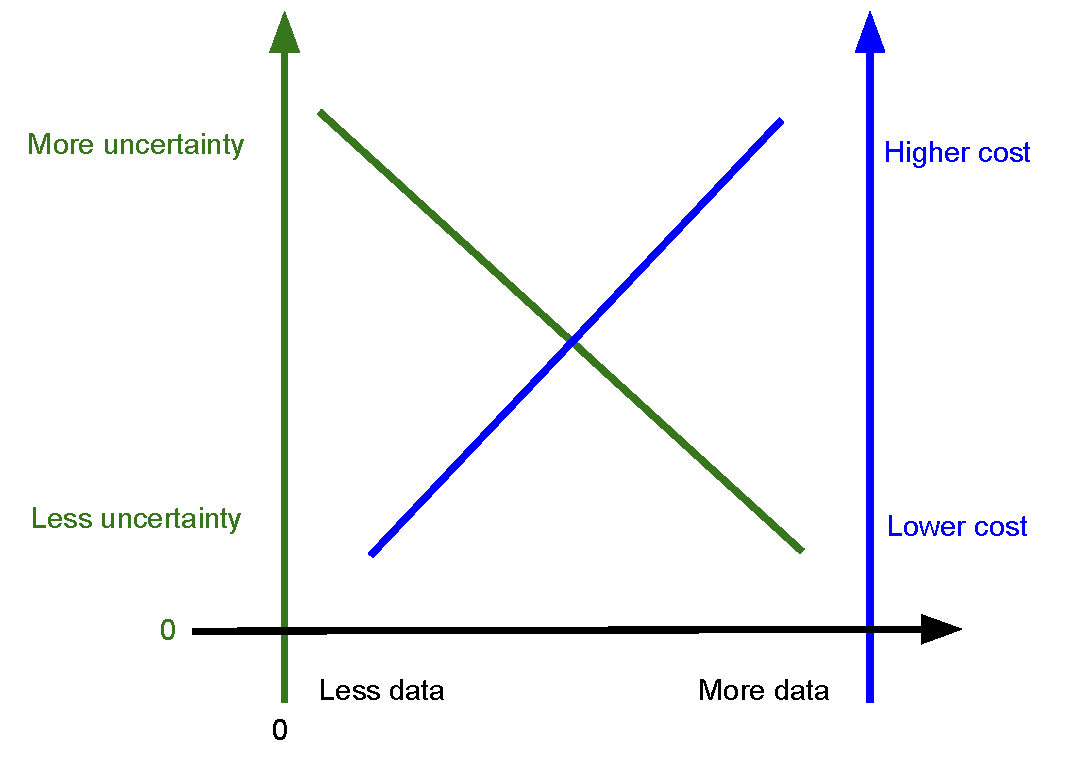
\includegraphics[width=0.8\textwidth]{images/cost_and_uncertainty_for_data_collection}
        \caption{Collecting more data costs money and decrease uncertainty. See Dilemma~\ref{table:gather_data_lots-vs-little}.}
        \label{fig:data_collection_cost_uncertainty}
\end{figure}

The logistics of gathering data can be measured, but there are other subjective aspects to account for as well. Making a decision has an emotional toll on the decider due to the risk of failure. Also, decisions are made in a social context, with decision makers accounting for the ramifications on people they have relationships with. 


Gathering data (Dilemma~\ref{table:gather_data_lots-vs-little}) is distinct from planning (Dilemma~\ref{table:planning}). It is possible to do a lot of planning with only a little information gathered, and it is feasible to have lots of data and do no planning. 

\begin{center}
\begin{table}[H] % ht
\begin{tabular}{ | m{\dilemmatablewidth}| m{\dilemmatablewidth} | } 
  \hline
  \textbf{Extensive planning upfront (proactive)} & 
  \textbf{Iterative improvement of plans (reactive)} \\ 
  \hline
  \textit{Description}: Lots of time spent brainstorming potential scenarios and contingency options prior to taking action. & 
  \textit{Description}: Start taking action and use feedback to shape next actions. \\ 
  \hline
  \textit{Cons}: ``No plan survives contact with the enemy.''\footnote{Modified from the original version written by \href{https://en.wikipedia.org/wiki/Helmuth_von_Moltke_the_Elder}{von Moltke}.} & 
  \textit{Cons}: Less prepared. \\  
  \hline
\end{tabular}
\caption{
\textit{Dilemma of Planning.}
\index{dilemma!of planning}
How much time to invest in planning.
%{\tiny Tag: Decision making.}
}
\label{table:planning}
\end{table}
\end{center}



\begin{center}
\begin{table}[H]
\begin{tabular}{ | m{\dilemmatablewidth}| m{\dilemmatablewidth} | } 
  \hline
  \textbf{Involve people who disagree.} & 
  \textbf{Ignore people who disagree.} \\ 
  \hline
  \textit{Pros}: Get constructive feedback; account for factors you didn't consider; build a robust solution. & 
  \textit{Pros}: Save time by not interacting. \\  
  \hline
  \textit{Cons}: Results in a compromise or partial solution that minimizes aggregate unhappiness. & 
  \textit{Cons}: Miss a vital aspect you didn't consider. \\  
  \hline
\end{tabular}
\caption{\textit{Dilemma of Disagreement.}
\index{dilemma!of disagreement}
Engagement with opposition to process or change.
%{\tiny Tag: Decision making.}
}
\label{table:opposition}
\end{table}
\end{center}

Making a decision imposes a bound on how much time is available for both gathering data and planning. Time is zero sum, so more time gathering data is less time planning. Similarly, the number of people available for data gathering and planning is bounded, and tasking people is a zero sum choice.

\begin{figure}[H] % ht
    \centering
    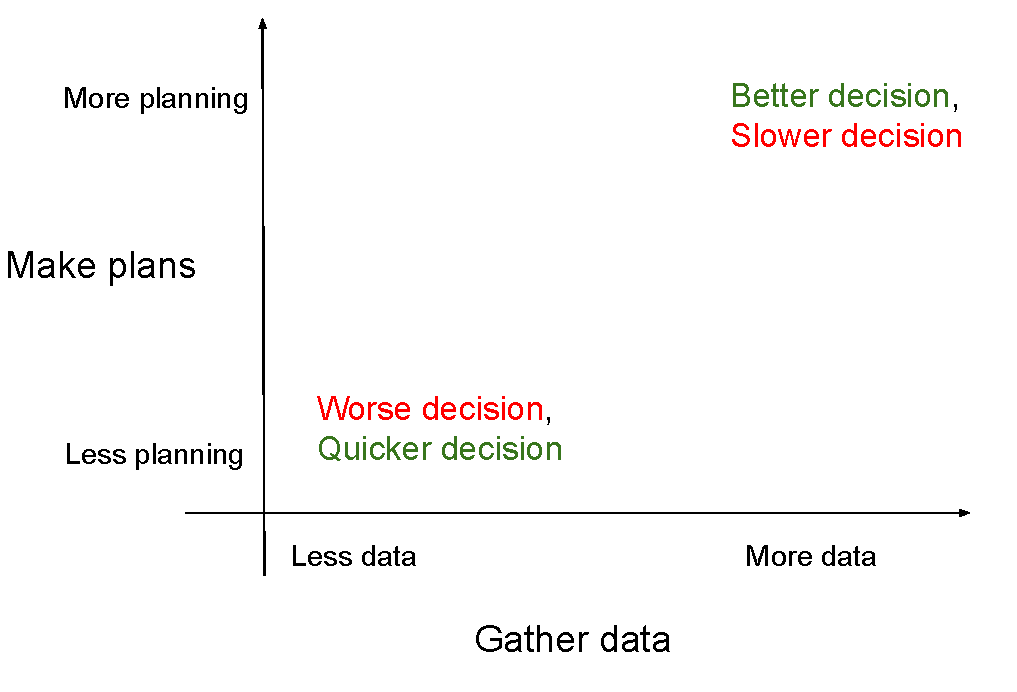
\includegraphics[width=0.8\textwidth]{images/planning_and_data_gathering.pdf}
    \caption{Planning (Dilemma~\ref{table:planning}) and data gathering (Dilemma~\ref{table:gather_data_lots-vs-little}) trade-off.}
    \label{fig:pareto_frontier}
\end{figure}

In practice, gathering data and planning rarely terminate -- they evolve.




When planning (Dilemma~\ref{table:planning}), aspects to consider include
%\begin{itemize}
%    \item 
the amount of risk seeking or tolerance (Dilemma~\ref{table:risk})
and
%    \item 
the intended scope of impact  (Dilemma~\ref{table:scope_broad-vs-narrow}).
%\end{itemize}

\begin{center}
\begin{table}[H] % ht
\begin{tabular}{ | m{\dilemmatablewidth}| m{\dilemmatablewidth} | } 
  \hline
  \textbf{Take on big risks and big rewards.} & 
  \textbf{Take on small risks and small rewards.} \\ 
  \hline
  \textit{Description}: High risk tolerance. &
  \textit{Description}: Low risk tolerance. \\
  \hline
  \textit{Pros}: Potential for failure and harm is significant. &
  \textit{Pros}: If any one investment fails, you can continue other efforts. \\
  \hline
  \textit{Cons}: Costly investment, longer feedback cycle. & 
  \textit{Cons}: Incremental can be slower. \\
  \hline
\end{tabular}
\caption{
\textit{Dilemma of \href{https://en.wikipedia.org/wiki/Risk_assessment}{Risk tolerance}.} 
\index{dilemma!of \href{https://en.wikipedia.org/wiki/Risk_assessment}{Risk tolerance}}
%{\tiny Tag: Personal choice.}
}
\label{table:risk}
\end{table}
\end{center}

\ \\

\begin{center}
\begin{table}[H] % ht
\begin{tabular}{ | m{\dilemmatablewidth}| m{\dilemmatablewidth} | } 
  \hline
  \textbf{Broad scope of impact.} &
  \textbf{Narrow scope of impact.} \\
  \hline
  \textit{Description}: The consequence of the work has many stakeholders. &
  \textit{Description}: Small number of stakeholders. \\  
  \hline
  \textit{Pros}: Benefit more people. &
  \textit{Pros}: Niche impact means less dependencies on other people. \\
  \hline
  \textit{Cons}: Harder to get everyone in agreement. & 
  \textit{Cons}: Less visibility to the rest of the organization. \\
  \hline
\end{tabular}
\caption{
\textit{Dilemma of Scope of Impact.}
\index{dilemma!of scope of impact}
Scope of impact of your work. 
%{\tiny Tag: Personal choice}
}
\end{table}
\label{table:scope_broad-vs-narrow}
\end{center}


Once data is gathered (Dilemma~\ref{table:gather_data_lots-vs-little}) and a plan is made (Dilemma~\ref{table:planning}), the result is disseminated. The choice on how to disseminate is Dilemma~\ref{table:consistency} and Dilemma~\ref{table:disseminate_one-by-one}.

\begin{center}
\begin{table}[H] % ht
\begin{tabular}{ | m{\dilemmatablewidth}| m{\dilemmatablewidth} | } 
  \hline
  \textbf{Guidance updated frequently; Incremental change.} & 
  \textbf{Consistent application of policy over time. Rules persist; then sudden drastic change.} \\ 
  \hline
  \textit{Pros}: Adapt policy to new information and changing conditions. &
  \textit{Pros}: Stability is easier to predict between regime changes.  \\
  \hline
  \textit{Cons}: More work needed. Accused of lacking stability. & 
  \textit{Cons}: Doesn't adapt as conditions change. Accused of being inflexible to evolving conditions. \\
  \hline
\end{tabular}
\caption{
\textit{Dilemma of Consistency over time.} 
\index{dilemma!of consistency over time}
Stability of rules; how change is implemented. Can also be characterized as when to tell other people: sooner or later (when firmer information is available).
See the description of 
\hyperref[sec:static-dynamic_processes]{static versus dynamic processes}.
\ifpageref
on page~\pageref{sec:static-dynamic_processes}
\fi
\ifsectionref
in section~\ref{sec:static-dynamic_processes} 
\fi
%{\tiny Tag: Organization's culture. Tag: Personal choice.}
}
\label{table:consistency}
\end{table}
\end{center}

Deployment of products and deployment of policies face similar dilemmas. \href{https://en.wikipedia.org/wiki/Diffusion_of_innovations}{Diffusion of Innovation}

\begin{center}
\begin{table}[H] % ht
\begin{tabular}{ | m{\dilemmatablewidth}| m{\dilemmatablewidth} | } 
  \hline
  \textbf{Tell people one-by-one.} & 
  \textbf{Tell everyone at once.} \\ 
  \hline
  \textit{Pros}: One-on-one allows a freer response from audience. &
  \textit{Pros}: Save time for the speaker. \\
  \hline
  \textit{Cons}: Order matters for relationships. & 
  \textit{Cons}: Overwhelming feedback all at once. \\  
  \hline
\end{tabular}
\caption{
\textit{Dilemma of Disseminating information.}
\index{dilemma!of disseminating information}
%{\tiny Tag: Personal choice.}
}
\label{table:disseminate_one-by-one}
\end{table}
\end{center}

Once a decision has been made, the decision is executed or enforced. How many rules are there (Dilemma~\ref{table:number_of_rules}) and
how strictly are the rules enforced (Dilemma~\ref{table:rule_strictness})?

\begin{center}
\begin{table}[H] % ht
\begin{tabular}{ | m{\dilemmatablewidth}| m{\dilemmatablewidth} | } 
  \hline
  \textbf{Enforce rules strictly.} & 
  \textbf{Lax rule enforcement.} \\ 
  \hline
  \textit{Pros}: Predictable. &
  \textit{Pros}: Bureaucrats feel empowered. \\
  \hline
  \textit{Cons}: Insensitive to nuance. & 
  \textit{Cons}: Tolerance for changing conditions or exceptional cases.  \\  
  \hline
\end{tabular}
\caption{
\textit{Dilemma of Strictness of rules.}
\index{dilemma!of strictness of rules}
%{\tiny Tag: Organization's culture.}
}
\label{table:rule_strictness}
\end{table}
\end{center}

\begin{center}
\begin{table}[H] % ht
\begin{tabular}{ | m{\dilemmatablewidth}| m{\dilemmatablewidth} | } 
  \hline
  \textbf{If it's not against the rules, it must be okay.} & 
  \textbf{I can only do what is allowed by the rules and nothing more.} \\ 
  \hline
  \textit{Pros}: Autonomy &
  \textit{Pros}:  \\
  \hline
  \textit{Cons}: . & 
  \textit{Cons}: .  \\  
  \hline
\end{tabular}
\caption{
\textit{Dilemma of Adherence to rules.}
\index{dilemma!of adherence to rules}
}
\label{table:rule_adherence}
\end{table}
\end{center}





\begin{center}
\begin{table}[H] % ht
\begin{tabular}{ | m{\dilemmatablewidth}| m{\dilemmatablewidth} | } 
  \hline
  \textbf{Control via rules.} & \textbf{Freedom/autonomy/agility.} \\ 
  \hline
  \textit{Description}: High number of rules to cover a variety of situations. & 
  \textit{Description}: Low number of rules to enable flexibility. \\ 
  \hline
  \textit{Cons}: The more rules that exist the more likely it is that someone will find a way to exploit them to their own advantage. & 
  \textit{Cons}: The fewer rules that exist the more likely it is that someone will try to get away with something bad. \\  
  \hline
\end{tabular}
\caption{
\textit{Dilemma of Number of rules.}
\index{dilemma!of number of rules}
%{\tiny Tag: Organization's culture}
}
\label{table:number_of_rules}
\end{table}
\end{center}
Alternative approach: guidance derived from principles that can be adapted to specific situations. That has the problem of requiring good knowledge of the situation and wise judgement.

\ \\

\begin{center}
\begin{table}[H] % ht
\begin{tabular}{ | m{\dilemmatablewidth}| m{\dilemmatablewidth} | } 
  \hline
  \textbf{I can only do what is mandated by the organization.} & 
  \textbf{I can do anything that's not illegal.} \\ 
  \hline
  \textit{Cons}: Responding to novel situations is inhibited. &
  \textit{Cons}:  \\  
  \hline
\end{tabular}
\caption{
\textit{Dilemma of Legality.}
\index{dilemma!of legality}
The scope of your actions bound by mandates and legality, but the way you interpret that is subjective.
}
\label{table:legality}
\end{table}
\end{center}
\ \\

\begin{center}
\begin{table}[H] % ht
\begin{tabular}{ | m{\dilemmatablewidth}| m{\dilemmatablewidth} | } 
  \hline
  \textbf{Decision in a process informed by a single bit of information.} & 
  \textbf{Fault tolerant decision making through redundancy.} \\ 
  \hline
  \textit{Cons}: Might be accidentally wrong. &
  \textit{Cons}: Extra burden of collecting and processing more data. \\  
  \hline
\end{tabular}
\caption{
\textit{Dilemma of Data for Decisions.}
\index{dilemma!of data for decisions}
Having a single checkmark on a form makes data collection easier. The person using the form might not see the checkmark box or may accidentally fill in the checkmark. The process is sensitive to this single bit of data.
}
\label{table:single-bit-decision}
\end{table}
\end{center}


\begin{center}
\begin{table}[H] % ht
\begin{tabular}{ | m{\dilemmatablewidth}| m{\dilemmatablewidth} | } 
  \hline
  \textbf{Quickly complete tasks or deploy new policies or create new products.} & 
  \textbf{Methodically complete tasks (or well-founded policies, quality products).} \\ 
  \hline
  \textit{Description}: Implement a solution quickly to address urgent needs. &
  \textit{Description}: Methodical well-planned design and execution yield robust solutions/products/policies. \\
  \hline
  \textit{Pros}: Rapid solution. &
  \textit{Pros}: More like to get the solution right. \\
  \hline
  \textit{Cons}: Risk of quick task is that the result is ineffective, inefficient, or wrong. &
  \textit{Cons}: \href{https://en.wikipedia.org/wiki/Opportunity_cost}{opportunity cost} \\  
  \hline
\end{tabular}
\caption{
\textit{Dilemma of Speed and Accuracy.}
\index{dilemma!of speed and accuracy}
Speed versus accuracy of task completion.
}
\label{table:quick-methodical}
\end{table}
\end{center}

If you try to resolve Dilemma~\ref{table:quick-methodical} by both getting a solution deployed quickly and then iterating towards a robust outcome, you may appear unpredictable or unstable; see Dilemma~\ref{table:planning}. This is an example of cascading dilemmas. The interplay of a creative resolution to one dilemma can impact the solution space for other dilemmas. 

\ \\

\begin{center}
\begin{table}[H] % ht
\begin{tabular}{ | m{\dilemmatablewidth}| m{\dilemmatablewidth} | } 
  \hline
  \textbf{Push people to work really hard.} & 
  \textbf{Create a comfortable work environment.} \\ 
  \hline
  \textit{Cons}: Burn out and leave. & 
  \textit{Cons}: Lower instantaneous productivity. \\  
  \hline
\end{tabular}
\caption{
\textit{Dilemma of Urgency.}
\index{dilemma!of urgency}
}
\label{table:rate-of-work}
\end{table}
\end{center}

\ \\

% https://bennorthrop.com/Essays/2022/code-ownership-stewardship-or-free-for-all.php
\begin{center}
\begin{table}[H] % ht
\begin{tabular}{ | m{\dilemmatablewidth}| m{\dilemmatablewidth} | } 
  \hline
  \textbf{Talk more to convey more information.} & 
  \textbf{Listen more to learn more information.} \\ 
  \hline
  \textit{Cons}: Less time available for listening. & 
  \textit{Cons}: Less time to convey what you know. \\  
  \hline
\end{tabular}
\caption{
\textit{Dilemma of Talking.}
\index{dilemma!of talking}
In conversations or meetings there is a (subjective) balance for participants.
}
\label{table:talk-or-listen}
\end{table}
\end{center}

\ \\


\begin{center}
\begin{table}[H] % ht
\begin{tabular}{ | m{\dilemmatablewidth}| m{\dilemmatablewidth} | } 
  \hline
  \textbf{Seek out experienced collaborators.} & 
  \textbf{Work with less experienced people.} \\ 
  \hline
  \textit{Pros}: Quicker to get something done. &
  \textit{Pros}: Less set in their ways and open to more novelty. \\  
  \hline
  \textit{Cons}: Experienced people who are good are probably busy. &
  \textit{Cons}: Slower progress. \\  
  \hline
\end{tabular}
\caption{
\textit{Dilemma of Experienced Collaborators.}
\index{dilemma!of experienced collaborators}
People with experience are useful but less accessible.
}
\label{table:experience}
\end{table}
\end{center}


\ \\

\begin{center}
\begin{table}[H] % ht
\begin{tabular}{ | m{\dilemmatablewidth}| m{\dilemmatablewidth} | } 
  \hline
  \textbf{Say yes to new opportunities.} & 
  \textbf{Say no to new opportunities.} \\ 
  \hline
  \textit{Pros}: Positive attitude, collaborative. &
  \textit{Pros}: Able to prioritize and focus. \\
  \hline
  \textit{Cons}: Fail to complete tasks. &
  \textit{Cons}: Not a team player. \\  
  \hline
\end{tabular}
\caption{
\textit{Dilemma of opportunities.}
\index{dilemma!of opportunities}
Acceptance or rejection of additional work can be explicit or implicit. Bureaucrats respond to this challenge by sending mixed signals: expressing interest but not following up with action.
}
\label{table:new-opportunties}
\end{table}
\end{center}

\ \\

\begin{center}
\begin{table}[H] % ht
\begin{tabular}{ | m{\dilemmatablewidth}| m{\dilemmatablewidth} | } 
  \hline
  \textbf{Share less data.} &
  \textbf{Share more data.} \\
%  \hline
%  \textit{Description}:  &
%  \textit{Description}:  \\  
  \hline
  \textit{Pros}: Restricting data access saves money for the data owner.&
  \textit{Pros}: Sharing data improves transparency and accountability. \\
  \hline
  \textit{Cons}: People other than the data owner are unable to extract value from data. & 
  \textit{Cons}: Sharing data uses resources (people, money, time). \\
  \hline
\end{tabular}
\caption{
\textit{Dilemma of Sharing Data.}
\index{dilemma!of sharing data}
How much data to share. Potential solution is to make data discoverable. Advertise the availability of data without providing data. This way a negotiation is feasible for people interested in the data.
%{\tiny Tag: Personal choice.}
}
\label{table:data_share-vs-hide}
\end{table}
\end{center}

In \ref{table:data_share-vs-hide} there is a lot of aspects of data than can be shared for discoverability: who to contact about access, what the data sources are, how frequently data is collected, how long data is stored, how much data there is.

\ \\

\begin{center}
\begin{table}[H] % ht
\begin{tabular}{ | m{\dilemmatablewidth}| m{\dilemmatablewidth} | } 
  \hline
  \textbf{Compete for resources.} &
  \textbf{Cooperate for productivity.} \\
  \hline
  \textit{Description}: individuals compete for attention and promotion; teams compete for money and staffing resources &
  \textit{Description}: cooperation improves productivity \\  
  \hline
  \textit{Cons}: Fail to synergize skills resources & 
  \textit{Cons}: Not clear who to assign responsibility for success or failure \\
  \hline
\end{tabular}
\caption{
\textit{Dilemma of Cooperate or Compete.} 
\index{dilemma!of cooperate or compete}
Applies to teams and to individuals. 
%{\tiny Tag: Personal choice.}
}
\label{table:cooperate-vs-compete}
\end{table}
\end{center}

\ \\

\begin{center}
\begin{table}[H] % ht
\begin{tabular}{ | m{\dilemmatablewidth}| m{\dilemmatablewidth} | }
  \hline
  \textbf{Consistent application of policy across cases.} &
  \textbf{Adapt policy to specific cases.} \\
  \hline
  \textit{Description}: Maximize broad applicability; minimize exceptions. &
  \textit{Description}: Demonstrate flexibility for unique scenarios. \\  
  \hline
  \textit{Cons}: Less sensitive to the nuances of a specific situation. & 
  \textit{Cons}: Takes more work. More likely to be accused of bias. \\
  \hline
\end{tabular}
\caption{
\textit{Dilemma of Consistent Policies.}
\index{dilemma!of consistency policies}
Case consistency vs adaptability.
%{\tiny Tag: Personal choice.}
}
\label{table:policy_consistency_across_cases}
\end{table}
\end{center}

When change to policies is desired, there are options on how to advocate for change -- Dilemma~\ref{table:how_to_change}.

% https://bennorthrop.com/Essays/2022/code-ownership-stewardship-or-free-for-all.php
\begin{center}
\begin{table}[H] % ht
\begin{tabular}{ | m{\dilemmatablewidth}| m{\dilemmatablewidth} | } 
  \hline
  \textbf{One person or team owns an area of responsibility.} & 
  \textbf{Anyone take on any task.} \\ 
  \hline
  \textit{Cons}: Staffing capacity may not be as flexible as varying workload. & 
  \textit{Cons}: Not everyone is skilled at everything. \\  
  \hline
\end{tabular}
\caption{
\textit{Dilemma of Swimlanes.} 
\index{dilemma!of swimlanes}
How are tasks assigned? This can be negotiated with coworkers and is not intrinsic to structure of the organization. 
}
\label{table:swimlanes}
\end{table}
\end{center}


Independent of how tasks are assigned within a team or organization (Dilemma~\ref{table:swimlanes}), individual bureacrats can decide how they act in Dilemma~\ref{table:scope_of_activity}.


\begin{center}
\begin{table}[H] % ht
\begin{tabular}{ | m{\dilemmatablewidth}| m{\dilemmatablewidth} | }
  \hline
% https://graphthinking.blogspot.com/2019/07/not-too-loose-not-too-tight-determining.html
  \textbf{Adhere strictly to the scope of your role.} & 
  \textbf{Stray outside (or outright ignore) the scope of your role.} \\ 
  \hline
  \textit{Description}: Inflexible to novelty. Specialization of tasking. & 
  \textit{Description}: Lack of structure. Generalization. \\ 
  \hline
  \textit{Cons}: Efficiencies of cooperation and specialization would not occur. & 
  \textit{Cons}: \href{https://en.wikipedia.org/wiki/Deadlock}{Deadlock} condition arises due to a scheduling constraint -- no one can proceed because everyone is waiting on everyone else. Responsibilities are unclear when no ones scope is clear. \\  
  \hline
\end{tabular}
\caption{
\textit{Dilemma of Scope.}
\index{dilemma!of scope}
Both strict adherence to role scope and ignoring scope can decrease an organization's productivity. 
What happens when a person deviates from their role?
How are people who do not conform identified? Are they confronted?
}
\label{table:scope_of_activity}
\end{table}
\end{center}

\begin{center}
\begin{table}[H] % ht
\begin{tabular}{ | m{\dilemmatablewidth}| m{\dilemmatablewidth} | } 
  \hline
  \textbf{Delegate; share work with other people.} & 
  \textbf{Work alone; don't rely on other people.} \\ 
  \hline
  \textit{Cons}: Your success is dependent on other people. & 
  \textit{Cons}: Can't accomplish as much on your own. \\  
  \hline
\end{tabular}
\caption{
\textit{Dilemma of Delegation.}
\index{dilemma!of delegation}
Sharing work can improve productivity and build relationships but also incurs risks to reputation and success.
}
\label{table:delegate-or-not}
\end{table}
\end{center}

\begin{center}
\begin{table}[H] % ht
\begin{tabular}{ | m{\dilemmatablewidth}| m{\dilemmatablewidth} | } 
  \hline
  \textbf{Many small tasks or objectives.} & 
  \textbf{Fewer big tasks or objectives.} \\ 
  \hline
  \textit{Description}: Your day is occupied with a variety of short-duration tasks. & 
  \textit{Description}: You work on only a few efforts during a typical day. \\  
    \hline
  \textit{Cons}: Enables a fail fast approach from quick feedback. & 
  \textit{Cons}: Less overhead of task switching to manage. \\
  \hline
\end{tabular}
\caption{
\textit{Dilemma of Chunk size.}
\index{dilemma!of chunk size}
You may or may not have a choice of task size and number of tasks. If you have autonomy, what do you prefer? Do your coworkers and supervisors know your preference? 
}
\label{table:chunk_size}
\end{table}
\end{center}

\begin{center}
\begin{table}[H] % ht
\begin{tabular}{ | m{\dilemmatablewidth}| m{\dilemmatablewidth} | } 
  \hline
  \textbf{Task with many external dependencies.} & 
  \textbf{Task with few external dependencies.} \\ 
  \hline
  \textit{Cons}: Risk of failing because of a failed dependency. & 
  \textit{Cons}: Have to develop everything yourself; waste of resources due to redundancy. \\  
  \hline
\end{tabular}
\caption{
\textit{Dilemma of Dependencies.}
\index{dilemma!of dependencies}
External dependencies can enable broader scope. This Dilemma only is relevant if you have autonomy in the selection of your tasks. See also the Dilemma of Delegation, \ref{table:delegate-or-not}.
}
\label{table:number_of_external dependencies}
\end{table}
\end{center}

\begin{center}
\begin{table}[H] % ht
\begin{tabular}{ | m{\dilemmatablewidth}| m{\dilemmatablewidth} | } 
  \hline
  \textbf{Focused on one role.} & 
  \textbf{Have multiple roles.} \\ 
  \hline
  \textit{Cons}: If a role does not consume 40 hours per week, you'll be idle. & 
  \textit{Cons}: Context switches between roles and delayed responses. \\  
  \hline
\end{tabular}
\caption{
\textit{Dilemma of Roles.}
\index{dilemma!of roles}
The right number of roles for a bureaucrat depends on personality and tasking. 
}
\label{table:number_of_roles}
\end{table}
\end{center}


\begin{center}
\begin{table}[H] % ht
\begin{tabular}{ | m{\dilemmatablewidth}| m{\dilemmatablewidth} | } 
  \hline
  \textbf{Dissent is welcome and discussed freely.} & 
  \textbf{Dissent is suppressed.} \\ 
  \hline
  \textit{Cons}: Can be disruptive to normal operations. Distracts from the task. & 
  \textit{Cons}: Limits novel ideas from spreading. Harms morale. \\  
  \hline
\end{tabular}
\caption{
\textit{Dilemma of Dissent.}
\index{dilemma!of dissent}
Dissent is caused by dissatisfaction with people or processes. 
}
\label{table:how_dissent_is_responded_to}
\end{table}
\end{center}


\begin{center}
\begin{table}[H] % ht
\begin{tabular}{ | m{\dilemmatablewidth}| m{\dilemmatablewidth} | } 
  \hline
  \textbf{Do share lessons learned.} & 
  \textbf{Don't share lessons learned.} \\ 
  \hline
  \textit{Pros}: Honesty, accountability, self-awareness, and self-reflection. & 
  \textit{Pros}: Look competent, even when making mistakes. \\  
  \hline
  \textit{Cons}: Looks weak, unprofessional. & 
  \textit{Cons}: Limit the growth of bureaucrats in the organization. \\  
  \hline
\end{tabular}
\caption{
\textit{Dilemma of Sharing Lessons.}
\index{dilemma!of sharing lessons}
Sharing lessons learned may seem reasonable unless you want to maintain a pristine reputation. 
}
\label{table:sharing_lessons_learned}
\end{table}
\end{center}

% https://graphthinking.blogspot.com/2019/07/vulnerability-of-organizations-in.html
\begin{center}
\begin{table}[H] % ht
\begin{tabular}{ | m{\dilemmatablewidth}| m{\dilemmatablewidth} | } 
  \hline
  \textbf{Share lessons learned about yourself.} & 
  \textbf{Share lessons learned from observing others.} \\ 
  \hline
  \textit{Cons}: Potentially look stupid. & 
  \textit{Cons}: Potentially hurts their reputation. \\  
  \hline
\end{tabular}
\caption{
\textit{Dilemma of Sharing.}
\index{dilemma!of sharing}
When sharing lessons learned (option 1 in \ref{table:sharing_lessons_learned}), the lessons do not have to be about you. 
}
\label{table:share_lessons_learned}
\end{table}
\end{center}

\begin{center}
\begin{table}[H] % ht
\begin{tabular}{ | m{\dilemmatablewidth}| m{\dilemmatablewidth} | } 
  \hline
  \textbf{Learn lessons from your own mistakes.} & 
  \textbf{Learn lessons from others (formal training).} \\ 
  \hline
  \textit{Cons}: Potentially look stupid; waste resources discovering what others already know. & 
  \textit{Cons}: Formal training may overemphasize irrelevant or impractical concepts. \\  
  \hline
\end{tabular}
\caption{
\textit{Dilemma of Learning.}
\index{dilemma!of learning}
How much formal training to invest in before learning by doing?
}
\label{table:lessons_learned_source}
\end{table}
\end{center}



\begin{center}
\begin{table}[H] % ht
\begin{tabular}{ | m{\dilemmatablewidth}| m{\dilemmatablewidth} | } 
  \hline
  \textbf{Build a small coalition of interested parties.} & 
  \textbf{Build a large base of support and get everyone on board.} \\ 
  \hline
  \textit{Cons}: May not be representative of all stakeholders. & 
  \textit{Cons}: Takes time away from the work. Many people may disagree or be disinterested. \\  
  \hline
\end{tabular}
\caption{
\textit{Dilemma of Coalitions.}
\index{dilemma!of coalitions}
A coalition can provide morale support but takes time to build.
%{\tiny Tag: }
}
\label{table:how_to_change}
\end{table}
\end{center}

\ \\

\begin{center}
\begin{table}[H] % ht
\begin{tabular}{ | m{\dilemmatablewidth}| m{\dilemmatablewidth} | } 
  \hline
  \textbf{Process request as they arrive.} &
  \textbf{Process request in batches.} \\
  \hline
%  \textit{Description}: . & 
%  \textit{Description}: . \\
%  \hline
  \textit{Pros}: Responsive. & 
  \textit{Pros}: Improves efficiency. \\
  \hline
  \textit{Cons}: Decreased efficiency. & 
  \textit{Cons}: Induces a delay in processing. \\
  \hline
\end{tabular}
\caption{
\textit{Dilemma of Batching.}
\index{dilemma!of batching}
For repeated actions, who is the process optimized for -- the subject or the bureaucrat?
}
\label{table:dilemma-of-batching}
\end{table}
\end{center}

\ \\

\begin{center}
\begin{table}[H] % ht
\begin{tabular}{ | m{\dilemmatablewidth}| m{\dilemmatablewidth} | } 
  \hline
  \textbf{Redundant reviews of data.} &
  \textbf{Single review of data.} \\
  \hline
  \textit{Description}: Multiple independent confirmations that the data collected is correct. & 
  \textit{Description}: A form featuring a checkbox option.  \\
  \hline
  \textit{Pros}: Decrease mistakes. & 
  \textit{Pros}: Less overhead. \\
  \hline
  \textit{Cons}: More people or time needed. & 
  \textit{Cons}: Single point of failure. \\
  \hline
\end{tabular}
\caption{
\textit{Dilemma of Redundancy.}
\index{dilemma!of redundancy}
If a user doesn't see a checkbox on a form, or they incorrectly mark the checkbox, is there any validation of the selection?
}
\label{table:dilemma-of-redundancy}
\end{table}
\end{center}


\subsection*{Dilemmas of Policy for an Organization's Structure\label{sec:org-dilemma}}

The constraints a decision maker faces are informed by the person's environment. Dilemmas \ref{table:people-per-supervisor} through \ref{table:market-vs-monopoly} shape the experience of bureaucrats in an organization.

\begin{center}
\begin{table}[H] % ht
\begin{tabular}{ | m{\dilemmatablewidth}| m{\dilemmatablewidth} | } 
  \hline
  \textbf{Flatter hierarchical organization.} &
  \textbf{More layers of hierarchy.} \\ 
  \hline
  \textit{Description}: More people managed per supervisor. & 
  \textit{Description}: Fewer people managed per supervisor. \\ 
  \hline
  \textit{Cons}: Less feedback/attention per employee. & 
  \textit{Cons}: Fewer people doing work. \\  
  \hline
\end{tabular}
\caption{
\textit{Dilemma of Shape of hierarchical organization.}
\index{dilemma!of flatness}
%{\tiny Tag: Organization's culture}
}
\label{table:people-per-supervisor}
\end{table}
\end{center}

\ \\

\begin{center}
\begin{table}[H] % ht
\begin{tabular}{ | m{\dilemmatablewidth}| m{\dilemmatablewidth} | } 
  \hline
  \textbf{Staffing: good coverage.} &
  \textbf{Staffing: minimal coverage.} \\
  \hline
  \textit{Description}: Sufficient staff. &
  \textit{Description}: As small of staff as possible. \\  
  \hline
  \textit{Pros}: Cover all edge cases; resilient to changing demands. &
  \textit{Pros}: Less expensive. \\
  \hline
  \textit{Cons}: Slack resources; sometimes inefficient. Increased communication needed. & 
  \textit{Cons}: Fragile when requirements change or workload increases. If one person departs and there's no redundancy, capacity and capability are harmed.  \\
  \hline
\end{tabular}
\caption{
\textit{Dilemma of Size of team or organization.}
\index{dilemma!of team size}
%{\tiny Tag: Design of organization.}
}
\label{table:staff_many-vs-few}
\end{table}
\end{center}


\ \\

\begin{center}
\begin{table}[H] % ht
\begin{tabular}{ | m{\dilemmatablewidth}| m{\dilemmatablewidth} | } 
  \hline
  \textbf{In-house services for non-central activities.} &
  \textbf{External dependencies for non-central activities.} \\
%  \hline
%  \textit{Description}:  &
%  \textit{Description}:  \\  
  \hline
  \textit{Pros}: More control. &
  \textit{Pros}: Easier to replace. \\
  \hline
  \textit{Cons}: Expands scope of responsibilities. & 
  \textit{Cons}: Less understanding of problem.  \\
  \hline
\end{tabular}
\caption{
\textit{Dilemma of Services.}
\index{dilemma!of services}
Services that are necessary but not central.
%{\tiny Tag: Design of organization.}
}
\label{table:inhouse-vs-external}
\end{table}
\end{center}

Table~\ref{table:inhouse-vs-external} isn't unique to bureaucracy. It applies to businesses in a market and to governments in a global environment. 

\ \\

\begin{center}
\begin{table}[H] % ht
\begin{tabular}{ | m{\dilemmatablewidth}| m{\dilemmatablewidth} | } 
  \hline
  \textbf{Centralized services.} &
  \textbf{Locally distributed services.} \\
  \hline
  \textit{Description}: A single provider of services for the organization; typically top-down mandate. &
  \textit{Description}: Each team has a local service provider; typically bottom-up organic result. \\  
  \hline
  \textit{Pros}: Cheaper. Enables coordination. &
  \textit{Pros}: Quicker response. 
  Enables innovation. 
  Accounts for local deviations from the norm. \\
  \hline
  \textit{Cons}: Less sensitive to local issues. Less responsive. Longer delays. Single point of failure.  & 
  \textit{Cons}: Uneven quality of service. Inconsistent strategies and policies. \\
  \hline
\end{tabular}
\caption{
\textit{Dilemma of Centralization of services.}
\index{dilemma!of centralization}
Oscillation (see figure\ref{fig:central-vs-distributed}) indicates neither solution is optimal.
%{\tiny Tag: Design of organization.}
}
\label{table:central-vs-distributed}
\end{table}
\end{center}

\begin{figure}[H] % ht
    \centering
    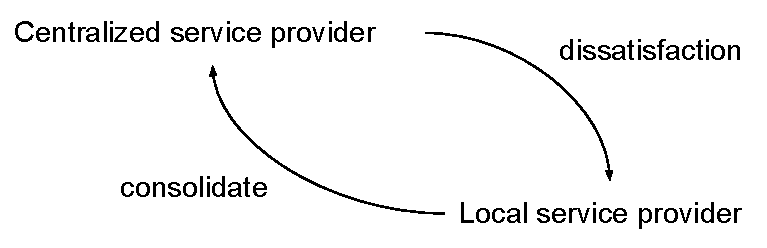
\includegraphics[width=0.8\textwidth]{images/dilemma_centralization-vs-distributed.pdf}
    \caption{Dipole oscillation. See Dilemma~\ref{table:central-vs-distributed}. Migrating to the opposite paradigm gives people in charge a chance to show their responsiveness to the needs of participants. The rate of oscillation is a measure of institutional memory half-life.}
    \label{fig:central-vs-distributed}
\end{figure}

Centralization is often carried out for the purposes of cost efficiency. The cost savings are due to de-duplication and having less slack. Both of those ``savings'' are a decrease of redundancy, which has a cost when there are unexpected fluctuations in need. 

Centralization is an intentional monopolization, with the corresponding decrease in choices. 
Centralization (de-localization) can decrease the value assigned to feedback from people using the service because personal relations are de-valued. 

The weaker feedback, lack of redundancy, and decreased emphasis on relationships motivates the creation of local services. 

\ \\

\begin{center}
\begin{table}[H] % ht
\begin{tabular}{ | m{\dilemmatablewidth}| m{\dilemmatablewidth} | } 
  \hline
  \textbf{Decision making lower in a hierarchy} &
  \textbf{Decision making higher in a hierarchy} \\
  \hline
  \textit{Description}: Push decisions down to empower employees. &
  \textit{Description}: Escalate every decision to management. \\  
  \hline
  \textit{Pros}: Better information. &
  \textit{Pros}: Better scope. \\
  \hline
  \textit{Cons}: more inconsistency & 
  \textit{Cons}: Decision maker has less skin in the game and may be less well informed. Employees are disempowered. \\
  \hline
\end{tabular}
\caption{
\textit{Dilemma of Decision height.}
\index{dilemma!of decision height}
Where decisions get made in hierarchical organization.
%{\tiny Tag: Design of organization.}
}
\label{table:decisions_low-vs-high}
\end{table}
\end{center}


\ \\

\begin{center}
\begin{table}[H] % ht
\begin{tabular}{ | m{\dilemmatablewidth}| m{\dilemmatablewidth} | } 
  \hline
  \textbf{Redundant services in a market} &
  \textbf{Monopoly service provider} \\
  \hline
  \textit{Description}: using a market model within the organization &
  \textit{Description}:  \\  
  \hline
  \textit{Pros}: enable customers to choose the best service &
  \textit{Pros}: efficiency of a single service \\
  \hline
  \textit{Cons}: redundancy & 
  \textit{Cons}: might not meet the needs of all customers \\
  \hline
\end{tabular}
\caption{
\textit{Dilemma of Monopoly.}
\index{dilemma!of monopoly}
Services within an organization. See also figure\ref{fig:market-vs-monopoly}.
%{\tiny Tag: Design of organization.}
}
\label{table:market-vs-monopoly}
\end{table}
\end{center}


\begin{figure}[H] % ht
    \centering
    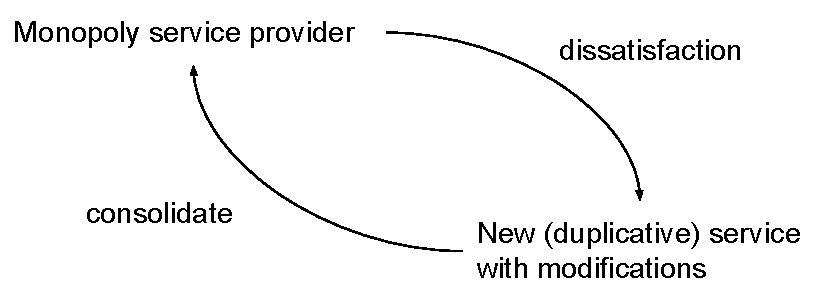
\includegraphics[width=0.8\textwidth]{images/dilemma_market_vs_monopoly.pdf}
    \caption{Dipole oscillation: solution A exists but doesn't meet my needs. Rather than tweak A, re-invent solution B which mostly overlaps with A but has independent development and support. See also Dilemma~\ref{table:market-vs-monopoly}.}
    \label{fig:market-vs-monopoly}
\end{figure}


% https://graphthinking.blogspot.com/2021/04/laffer-curve-and-minimum-viable.html
There is a Goldilocks situation for amount of processes in an organization:
\begin{itemize}
    \item Too few processes (all social relationships).
    \item Just the right amount -- a balance process and social, and when to use which is known.
    \item Too much process (not enough leveraging of social relationships)
\end{itemize}
This optimization is similar to the \href{https://en.wikipedia.org/wiki/Laffer_curve}{Laffer curve} in economics.

\ \\

\textit{Trilemma}: \textbf{Do you support the cutting edge, most of the middle, or the laggards?}\\
\index{trilemma!cutting edge, middle, laggards}
For any given aspect of bureaucracy there is a \href{https://en.wikipedia.org/wiki/Normal_distribution}{bell curve} of skills and interest of bureaucrats. In your role of bureaucrat you face a choice: find and collaborate with and enable the best and brightest, or aim your efforts at the massive mediocre middle (most bureaucrats), or try to get the dumbest bureaucrats up to speed? 

Attempting to escape the trilemma by claiming that you treat everyone equally means you are disregarding the needs of the tail of the distribution. 

\ \\

% https://graphthinking.blogspot.com/2021/12/hierarchical-organization-trilemma.html
\textit{Trilemma}: \textbf{Do you work for your team, your manager, or yourself?} \\
\index{trilemma!team, manager, yourself}
Being a member of a team that operates within a hierarchy is tough. One reason is the question of who you are working for. The trilemma is whether you work for yourself, work for your supervisor, or work for your team.  Ideally you can find ways to do all three, but that is not always the case. 

Members of the team should work collaboratively, but there is a potential counter-force: accountability to the supervisor. Because each team member is accountable to their supervisor(s), that motivates the action of the individual. The team does not actually have autonomy -- they are accountable to the boss.

In the approach ``team members are directed by their supervisor," the synergy of the team is neglected and the supervisor becomes a bottleneck (for decision making and for creativity and for planning).

The third approach is for a person to ignore their team and their supervisor. This might enable quicker progress, at the risk of going in an unhelpful direction or not leveraging skills of coworkers. 

\ \\

\textit{Trilemma}:
\textbf{Seek less budget, same, or larger budget.} 
\index{trilemma!less, same, or larger budget}
Less budget is needed if you improved efficiency, but then the proportional power within the organization is decreased. A larger budget may be due to inefficiency or growth. Keeping the same budget indicates no promotions are relevant (although a steady state could result from a combination of growth and improved efficency). 

\ \\

A trilemma applicable to many situations is that options are \textbf{fast, inexpensive, good; choose two}. 
\index{trilemma!fast, inexpensive, good}
(This is the \href{https://en.wikipedia.org/wiki/Project_management_triangle}{Project management triangle}.) \\
\index{folk wisdom!\href{https://en.wikipedia.org/wiki/Project_management_triangle}{Project management triangle}}
In other words, the options are
\begin{itemize}
    \item Good and fast is expensive (i.e., requires lots of resources).
    \item Good and inexpensive takes a long time (i.e., find a clever solution).
    \item Fast and inexpensive will be low quality.
\end{itemize}

\subsection*{Dilemmas Raised by Subjects of Bureaucracy\label{sec:subjects_dilemmas}}

Each subject of bureaucracy views themselves as logical and self-consistent and erudite. In practice, the bureaucrat servicing subjects encounters conflicting statements. 

\begin{center}
\begin{table}[H] % ht
\begin{tabular}{ | m{\dilemmatablewidth}| m{\dilemmatablewidth} | } 
  \hline
  \textbf{Subject: Why do I have to fill out this form?} &
  \textbf{Subject: Why aren't you catching more cheaters and fraudsters?} \\
  \hline
  \textit{Description}:  & 
  \textit{Description}:  \\
  \hline
  \textit{Pros}: . & 
  \textit{Pros}: . \\
  \hline
  \textit{Cons}: . & 
  \textit{Cons}: . \\
  \hline
\end{tabular}
\caption{\textit{Dilemma of forms.}
}
\label{table:dilemma-forms}
\end{table}
\end{center}

\ \\

\begin{center}
\begin{table}[H] % ht
\begin{tabular}{ | m{\dilemmatablewidth}| m{\dilemmatablewidth} | } 
  \hline
  \textbf{Subjects desire consistency across situations.} &
  \textbf{Subjects seek exceptions for their specific situation.} \\
  \hline
  \textit{Pros}: . & 
  \textit{Pros}: . \\
  \hline
  \textit{Cons}: . & 
  \textit{Cons}: . \\
  \hline
\end{tabular}
\caption{\textit{Dilemma of Consistency.}
Consistency is seen as fairness, when in fact consistency can ignore critical differences. Consistency is desirable for enabling predictability.
}
\label{table:dilemma-consistency}
\end{table}
\end{center}

\ \\

\begin{center}
\begin{table}[H] % ht
\begin{tabular}{ | m{\dilemmatablewidth}| m{\dilemmatablewidth} | } 
  \hline
  \textbf{Subjects seek clearly defined rules} &
  \textbf{Subjects seek flexibility in application of rules (because we have a personal relationship} \\
  \hline
  \textit{Description}: Rules are seen as enabling fairness, when in fact rules can perpetuate inequality. Rules (assuming uniform enforcement) are also seen as enabling predictability. & 
  \textit{Description}:  \\
  \hline
  \textit{Pros}: . & 
  \textit{Pros}: . \\
  \hline
  \textit{Cons}: . & 
  \textit{Cons}: . \\
  \hline
\end{tabular}
\caption{\textit{Dilemma of flexible rules.}
}
\label{table:dilemma-flexiblity}
\end{table}
\end{center}

\ \\

\begin{center}
\begin{table}[H] % ht
\begin{tabular}{ | m{\dilemmatablewidth}| m{\dilemmatablewidth} | } 
  \hline
  \textbf{Subject wants transparency.} &
  \textbf{Subject wants Low cost (free).} \\
  \hline
  \textit{Description}: Transparency requires collection and reporting of data. & 
  \textit{Description}:  \\
  \hline
  \textit{Pros}: . & 
  \textit{Pros}: . \\
  \hline
  \textit{Cons}: . & 
  \textit{Cons}: . \\
  \hline
\end{tabular}
\caption{\textit{Dilemma of transparency.}
Transparency has a cost.
}
\label{table:dilemma-transparency}
\end{table}
\end{center}




\subsubsection{Consequences of the Dilemma-based Framing}

The dilemmas listed above are numerous but not exhaustive. Even if each bureaucrat considers the same choices (which doesn't necessarily happen), not everyone makes the same selection. One response might be to defer to someone higher in the hierarchy to coordinate. While this would ensure consistency, this would be \href{https://en.wikipedia.org/wiki/Micromanagement}{micromanagement}. The people in the hierarchy above the person facing the choice don't have exposure to the problem. Choices are delegated to leverage expertise. 

\ \\

When you are facing these dilemmas and trilemmas\marginpar{[Tag] Actionable Advice} there are constructive responses that can improve your effectiveness. Improvement benefits your results, your reputation, and the organization. 
\begin{itemize}
    \item Collect quantitative data for each variable. Quantitative arguments can augment qualitative stories. 
    \item Construct the Pareto frontier to identify non-optimal choices that can be eliminated.
    \item Instead of assessing variables in isolation, assess consequences in the context of workflows and impacts on stakeholders.
    \item Discuss subjective decisions with stakeholders so that potential disagreements can be negotiated instead of creating friction.
\end{itemize}
 

 \clearpage
  \subsection{Unavoidable Hazards of Bureaucracy\label{sec:unavoidable_hazards}}

Inefficiency of changing the requirements on a project partway through. If an objective quantitative measure were available, the ROI could be determined.  \clearpage
  \section{How to be an Effective Bureaucrat\label{sec:effective_bureaucrat}}

So far I've described dilemmas in \S\ref{sec:dilemma_trilemma} and unavoidable hazards in \S\ref{sec:unavoidable_hazards}. Given this nuanced view of the complexity of bureaucracy, how can you leverage that insight?

Baseline assumptions are that you are a good person, you are technically skilled at your technical duties, and you are a good project manager. 


Superpowers of a bureaucrat in a bureaucratic organization that facilitate cooperation and progress:

\begin{itemize}
\item You strive for and demonstrate transparency. You share information with stakeholders.
\item You seek information from stakeholders.
\item You apply consistent processes (rather than being reactionary and applying ad hoc responses).
\item You hold others (and yourself) accountable for their actions.
\item You account for varying incentives and reference experiences.
    \item You communicate more effectively than anyone around you.
    \item Your effectively multi-task, or, more accurately, switch tasks. The switch among tasks is triggered when the current task encounters an externally-generated pause. You can \href{https://en.wikipedia.org/wiki/Pipeline_(computing)#Concept_and_motivation}{pipeline your activities}.
    \item You are prepared with a backlog of ideas (in writing) if someone shows up with resources.
    % https://graphthinking.blogspot.com/2016/12/life-lessons-i-learned-from-experience.html
    \item If you are dependent on someone else getting something done to enable your progress, you can demonstrate priority by physically show up -- \underline{presence creates priority}. Being physically at a person's desk motivates that person to respond better than calling them or emailing them. Showing up where someone works and talking with them conveys how much priority you place on the actions of the person you're talking with.
    \item You reply quickly to incoming requests. This allows other people's tasks to either be resolved or have a clear response about when progress can be expected. 
    \item You have intellectual empathy -- theory of mind for thinking (whereas empathy refers to emotions). How to grow your intellectual empathy: shadow peers and bosses
    \item You have process empathy. Observe deviations and exceptions that cause processes to come into existence. 
    \item You avoid unintentionally dropping tasks or requests. This requires capturing incoming requests and then providing a response about prioritization and status. This matters because other participants in the organization should regard you as reliable in a positive sense. 
    \item You focus on value delivery in relationships that exceed the scope of your formal role.
\item You have altered your job description to fit the growth you're seeking.
\item You are willing to engage on a personal level and know someone outside their professional role.
\item Each of your tasks have a customer, a deadline, and a deliverable.
\item You occasionally ponder and discuss with other people introspective questions like
\begin{itemize}
    \item How can I be successful?
    \item What are the ways I could fail?
    \item How the organization is regarded as successful?
    \item What are the ways the organization can fail?
\end{itemize}
% https://graphthinking.blogspot.com/2017/07/questions-to-ask-mentors.html
\item You find mentors and ask them questions like
\begin{itemize}
    \item What do you like most about your career? 
    \item Given the chance, what would you do differently?
    \item How do you manage work/life balance?
    \item What's the big challenge for our industry in the next two years?
    \item How would you tackle that challenge?
    \item What advice do you have for a young person starting in this industry? Mistakes to avoid?  How to be successful?
    \item What books would you recommend reading?
\end{itemize}
\end{itemize}


A bureaucrat can accomplish more as part of an organization than by working alone. Being a member of an organization means the bureaucrat's identity is subsumed into service for the organization they are part of~\footnote{\href{https://en.wikipedia.org/wiki/Deindividuation}{Deindividuation}}. At the same time, bureaucracy enables the bureaucrat to amplify their presence by being part of a larger organization.  Sometimes the cost of being part of the organization exceeds the force multiplier of working together. 




% https://graphthinking.blogspot.com/2019/05/definition-of-progress.html
Measuring your own personal growth in a bureaucracy is difficult due to the lack of feedback loops. One approach is to measure your capabilities with respect to a specific task. If you can complete the task in less time and with fewer resources and with less effort, that's progress. If you can now complete a task that you previously wanted to but weren't able to, that's progress.



Bureaucracy induces emotional response in participants because things don't work they way each person wants. This can lead emotionally to frustration and then apathy. Understanding how things operate in a bureaucracy can help decrease the anger.

% Wandering the maze of bureaucratic processes as a subject.

Another emotional response to bureaucracy is a sense of powerlessness. 
\begin{quote}
Some third person decides your fate: this is the whole essence of bureaucracy.\footnote{``The Workers' Opposition'' by Alexandra Kollontai, 1921}
% https://alphahistory.com/russianrevolution/kollontai-on-soviet-bureaucracy-1921/
\end{quote}
That sense of powerlessness applies both to bureaucrats and to subjects of bureaucracy. 

The sense of powerlessness is somewhat valid, in that you are as a bureaucrat giving up some power compared to your ability to act individually. That is the trade for working with others

\ \\

A process feels bureaucratic when the subject is exposed to more than one step to get something done that if one person were doing it would be simpler. Consolidation from the subject's perspective decreases the apparent bureaucracy. The barrier to implementation is the necessary coordination among different stakeholders who receive no benefit from the coordination. Externalizing the coordination to the subject is what causes the sense of bureaucracy. 


\ \\

Don't rely on one person or one idea for your success. On the other end of the spectrum, don't spread yourself too thin. 

\ \\

What to do when you get stuck?\\
look up stream, look downstream, look to peers

\ \\

When you are asked to take on additional work, avoid responding with ``that's not my job." If the request is misguided and your perception is that is really is the responsibility of another person, ask if the requester is aware of that other person's responsibilities. If you are to really take on the work, get guidance on re-prioritizing and make sure the request is documented in writing. 

\ \\

If there's something you want to accomplish, strive for influence without authority instead of working to gain control over resources (e.g., through promotion). Avoid the following: ``In this organization X is important to me, but I can't do X right now because I don't have enough power in the org. So I'll get promoted and then do X."

\ \\



\textit{TODO}: \textbf{Learn the perspectives of those around you.}\\
The relevance of knowing the paradoxes including dilemmas and unavoidable hazards, is that you should talk explicitly to your fellow bureaucrats about these specific topics in conversation. Not that the goal is to find consensus or agreement. But to find what the other person is thinking so that you can account for their processes


\textit{TODO}: \textbf{Account for holistic view}\\
The specific circumstances of the challenges you face as a bureaucrat depend on the individual people involved, what the purpose of the bureaucracy is, what technology is available for implementation of bureaucracy, and the resources (staffing, money, time). 

\textit{TODO}: \textbf{Learn the history of the problem}\\
This goes beyond Chesterton's fence, which focuses about why the current approach is in placed. Learning the history of a problem means what has been tried before and failed? How did the previous iterations evolve into the current situation? Was the cause personalities, insufficient resources, inadequate technology? What's changed that enables this approach to be better? What do you know that prior attempts didn't?

\textit{TODO}: \textbf{Concurrently work on 3 remedies}\\


\textit{TODO}: \textbf{Minimize \href{https://en.wikipedia.org/wiki/Externality}{external costs}}\\
A solution that externalizes costs harms the greater organization and creates bureaucratic debt.


\textit{TODO}: \textbf{Exploit the flexibility of rules for the benefit of all parties.}\\
% https://graphthinking.blogspot.com/2019/07/winning-game.html
change the rules of the game and the objectives of the game such that every participant wins.

\textit{TODO}: \textbf{Align selfish interests with social interests.}\\
See also nudges. 
(Page 66 of \cite{2012_Schneier})

\textit{TODO}: \textbf{Find ways to rephrase negative complaints.}\\
% https://graphthinking.blogspot.com/2019/07/how-to-rephrase-negative-observations.html
Negative observation: "Logging into my computer takes a long time."\\
Positive statement and explanation of impact: "If the latency for logging into my computer were lower, I could make more progress on X."


Negative observation: "The service team I need support from doesn't offer a ticketing queue."\\
Positive statement: "If the service team I need support from offered a ticketing queue, I would be able to track the work done on my behalf."

\textit{TODO}: \textbf{Share lessons learned}\\ \clearpage

\chapter{Bureaucracies are made of Humans\label{b_made_of_humans}}
% instead of presenting specific lessons, here I'm going to present insider perspectives on the fundamentals described in previous chapters. 

This chapter provides an insider's perspective of working in a bureaucracy. What are all the aspects to consider?
% unordered essays to be clustered later

  \section{Getting started in a Bureaucracy}
    This section focuses on a bureaucrat's initial exposure to bureaucracy. 
  
    \subsection{What to Read\label{sec:to_read}}

The content of this book is independent of the specific role you as a bureaucrat will be playing. I assume you are striving to be a good person, and that you have relevant education/experience for the position in the organization.

The reading lists 
\href{https://github.com/LappleApple/awesome-leading-and-managing}{Leading and managing}, 
\href{https://github.com/kdeldycke/awesome-engineering-team-management}{Engineering team management}, 
\href{https://github.com/pdfernhout/High-Performance-Organizations-Reading-List}{High Performance Organizations}, and 
\href{https://github.com/ankitjaininfo/awesome-managers}{Managers}
are outside the scope of a guidebook for bureaucracy. 
%Bureaucracy involves hierarchy, so understanding the mechanics and nuances of hierarchical roles is useful. 


%Books on management might not seem applicable if you are not already in a management role.
Reading management books is helpful regardless of whether you are a manager, want to become a manager, or if you never want to become a manager. In all three cases, gaining awareness of best practices and alternative approaches benefits you as a bureaucrat and the people you coordinate with -- bosses, peer bureaucrats, subordinates, and subjects.

    \subsection{Hiring into a Bureaucracy}

Hiring shapes the culture of an organization and determines what is feasible, both by the skills of those hired and how well new hires integrate with the existing organization. 

Hiring is an expensive process in terms of money, time, emotional investment of candidates, and the burden of reviewing applicants. 
% SO WHAT? What's the consequence?

When hiring into an organization there is a selection bias in the people who join a bureaucracy, and there is a selection bias who stays in bureaucracy. 
% SO WHAT? What's the consequence?



Regardless of the specifics of the job, there are specific attributes that make a candidate more likely to be successful in a bureaucracy. In addition to role-specific skills, hire for \href{https://en.wikipedia.org/wiki/Metacognition}{metacognition}, social skills, and intrinsic motivation.

% https://graphthinking.blogspot.com/2021/04/screening-for-metacognition-in-job.html

% https://graphthinking.blogspot.com/2021/07/screening-for-intellectual-empathy-in.html

% https://graphthinking.blogspot.com/2021/04/questions-to-ask-interviewer-when.html


    \subsection{Promotion}

Promotion is a critical aspect of designing incentives for behavior. Promotion is central because there are a variety of motives -- for money, for status, for authority. 

promotion of individual (rather than team) results in hero culture

What is preventing innovation is lack of risk taking. Actual risk means potential for failure. fear of failure because culture avoids failure due to concerns of waste. Also, anyone who fails can use this argument, but that isn't the same as ``fail fast'' because what's critical is learning from failure and sharing that insight gained so other's don't need to repeat. 

two options for learning: your own mistakes, or the mistakes of others. "formal education" is about the latter

    \subsubsection{Organization chart orientation
\label{org-chart-orientation}}

A common method of describing relations within the bureaucracy is the organization chart (colloquially, the ``org chart"). Normally the CEO is at the top of the chart, middle management is in the middle, and managed employees are at the bottom. See figure~\ref{org_chart_orientation_ceo-at-top} 


An organization's culture is subtly conveyed by artifacts like org charts. 
% What's the point of this section? Is there a consequence, or is this just an observation?
There are emotional connotations to alternative layouts. You can alter expected relations (culture and norms) by playing with orientation of the org chart.
Org chart orientation can be overanalyzed, so this exploration is limited.

The point of thinking about org chart orientation is to frame how you perceive your supervisors, peers, subordinates. Notice that the framing is embedded in the words -- prefixes super (over) and sub (under). 
These concepts inform what you expect from relations.
Do I seek support or direction and guidance from my boss? What do I expect from my boss, peers subordinates? What do I expect to provide them?

%\begin{itemize}
%\item 
%\end{itemize}

The relative orientation of the \href{https://en.wikipedia.org/wiki/Chief_executive_officer}{CEO} to workers sets expectations for relations. 
Options for orientation are the conventional CEO at top
(figure~\ref{org_chart_orientation_ceo-at-top}), 
CEO at the bottom (figure~\ref{org_chart_orientation_ceo-at-bottom}),
CEO on the right (figure~\ref{org_chart_orientation_ceo-leads}),
CEO on the left (figure~\ref{org_chart_orientation_ceo-follows}),
CEO as the center of a star 
(Example: \href{https://en.wikipedia.org/wiki/File:League_of_Nations_Organization.png}{League of Nations diagram})

\begin{figure}
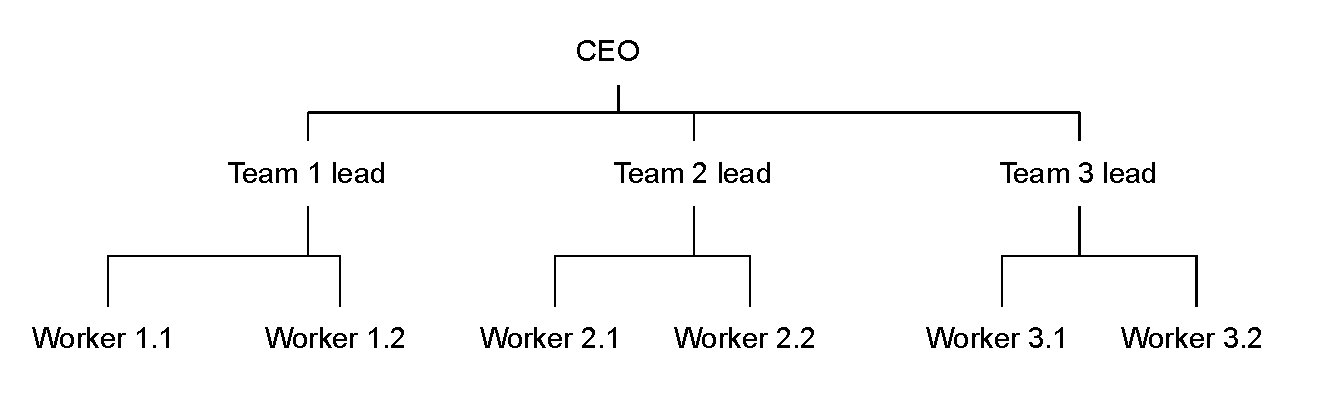
\includegraphics[width=1\textwidth]{images/org-chart-orientation-ceo-at-top.pdf}
\caption{Standard orientation. Role with most responsibility and authority is at top. Left-right ordering is intended to be irrelevant in this view, though left-to-right reading order emphasizes importance.}
\label{org_chart_orientation_ceo-at-top}
\end{figure}

\begin{figure}
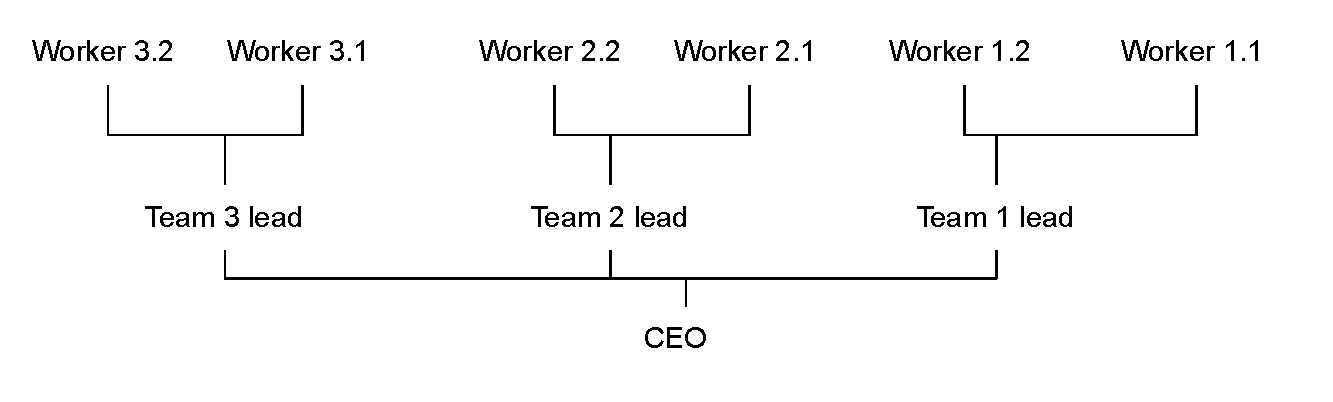
\includegraphics[width=1\textwidth]{images/org-chart-orientation-ceo-at-bottom.pdf}
\caption{Flipping the orientation presents a more realistic view of the CEO's responsibility. The crushing burden of servant leadership is clear. Left-right ordering is intended to be irrelevant in this view.}
\label{org_chart_orientation_ceo-at-bottom}
\end{figure}

\begin{figure}
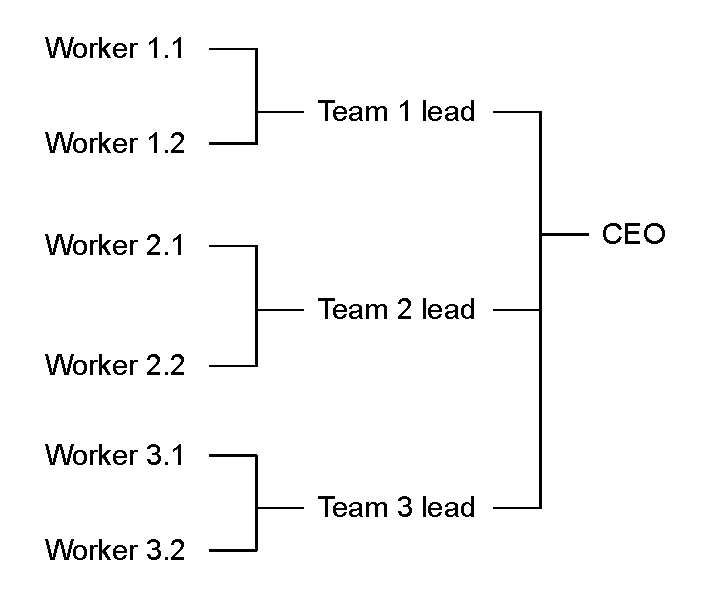
\includegraphics[width=0.8\textwidth]{images/org-chart-orientation-ceo-leads.pdf}
\caption{Conventionally time flows from left (old) to right (new), so in this graph the CEO leads the charge into the unknown. Is the CEO dragging workers forward, or are the workers pushing the CEO? The top-to-bottom ordering can be read as importance. }
\label{org_chart_orientation_ceo-leads}
\end{figure}

\begin{figure}
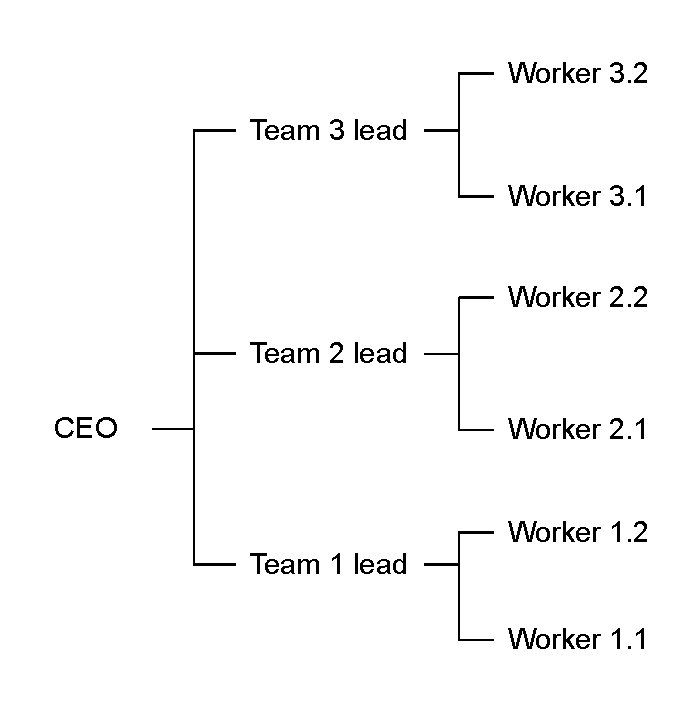
\includegraphics[width=0.8\textwidth]{images/org-chart-orientation-workers-lead.pdf}
\caption{The ``chariot view'' with the CEO in the chariot and the workers out front. Workers are in the future, the CEO is in the past operating on old information. As with figure~\ref{org_chart_orientation_ceo-leads}, top-to-bottom ordering can be read as importance. }
\label{org_chart_orientation_ceo-follows}
\end{figure}



%extension of 
% \href{https://en.wikipedia.org/wiki/Conway\%27s_law}{Conway's law}: seating chart reflects org chart
    \section{professional training}
  \newpage
  \section{You are an Individual in an Organization}
  
    This section focuses on the individual bureaucrat operating within an organization. 
    
    There is no neutral member of a bureaucracy. Either you are contributing to the organization, or you are sapping resources from the organization. This is because the organization operates in a zero-sum game for resource allocation.
    \subsection{Ideas for Innovation within a Bureaucracy\label{sec:innovation}}


The innovation lifecycle in a bureaucracy is
\begin{enumerate}
    \item You observe problems and challenges in your environment. This manifests as complaints from both the people directly harmed and observers who see inefficiency.
    \item You share ideas for innovation and gets feedback. Build a coalition of people willing to fight for the idea on your behalf
    \marginpar{[Tag] Actionable Advice}
    so that when you're not present, the idea is still proceeding towards implementation.  That puts the threshold at ``so important other people are willing to pause whatever they were working on and take up your cause.''
    \item Implementing these suggestions require either a change to existing processes or new processes or an investment of work. These changes may not succeed -- there's risk. Your idea could fail because it's not a good idea. It could also fail because someone doesn't like you, or the idea doesn't account for some dependency you weren't aware of, or it might conflict with other changes in progress.
    \item If you do decide to invest effort, the activity takes you away from your current work. Implementing the change might involve skills you don't have; learning those skills takes time. Carrying out the activity with new skills increases the likelihood of novice mistakes.
    \item If someone else implements the idea they get the credit for having done the work.
    \item If the idea saves money or time, there's typically no monetary reward. Recognition and benefit to your reputation isn't required as part of the change process. 
\end{enumerate}

There are many barriers in that lifecycle. The problem has to be observable to someone willing to invest effort in change. That person has to build a coalition of stakeholders. If the person isn't negatively harmed, that person may also lack clear benefit from resolving inefficiency. 

In addition to the work of implementing the change, there is an administrative overhead of documenting the reason for the change. 
Subjective decisions mean choices have to be defensible. 
The need for defensible justifications result in conservative decisions and risk aversion and a decrease of motive for innovation. 



These barriers lead to external observers to conclude something like the following simplification:
\begin{quote}
Bureaucracy destroys initiative. There is little that bureaucrats hate more than innovation, especially innovation that produces better results than the old routines.
\marginpar{[Tag] Folk wisdom}
Improvements always make those at the top of the heap look inept. Who enjoys appearing inept?\footnote{Frank Herbert (1987). ``Heretics of Dune'', page 201, Penguin}
% https://www.azquotes.com/quote/453163
\end{quote}


    \subsection{Motivation of Bureaucrats}

To understand the bureaucrats you work with, appreciating their diverse motives is instructive. If you expect everyone to have the same motives as you, then you will be surprised by the friction. 

Motivations of participants are rarely ``how can I make the company more successful" or even ``how can I sell/produce more product"? Usually motivation is based on personal success in various manifestations, which leads to emergent phenomena which appears confounding to observers outside the bureaucracy. 


% see https://en.wikipedia.org/wiki/Social_influence

Each bureaucrat has a motive, even the bureaucrats who do nothing. 
% https://graphthinking.blogspot.com/2020/02/there-is-no-idle-status-for-paid.html
In an organization where you are a paid bureaucrat, you are either actively working for improvement of the organization, or your existence is parasitic to the organization. There is no ``idle" status for paid employees in an organization with limited resources.

Not too efficient such that I eliminate the need for my job, and not so inefficient that the organization fails and I lose my job. Increasing the efficiency of bureaucracy is good for the organization and the outcomes, but can be harmful to the bureaucrat's career.

Career stability within an organization is a benefit, and it can be leveraged to take more risk. However, it typically manifests as inaction by an employee. There's no harm to the employee in not taking action. If an employee doesn't do anything, nothing bad will happen to that employee. Career stability decreases extrinsic motivation.



Example motivations for bureaucrats: stability, money, travel, problem solving, like being associated with org, logistical convenience (``the office is near where I lived.'')


    % management isn't leadership
    \subsection{Creating change in the organization\label{sec:creating_change}}

If the organization you are a participant in has no problems or challenges, this subsection can be skipped. For bureaucrats in organizations that do have structural problems, this part of the guidebook provides points to ponder independent of the specific problem.

As a bureaucrat, you have unique insight on the problems the organization faces, and you have unique leverage to alter the situation.  While you could proceed haphazardly, an effective bureaucrat has vision, goals that break down the vision, plans on how to achieve each goal, and milestones which indicate whether the plan is proceeding. 

Perspectives to consider when assessing change include what the situation is, what the situation could be, and what the situation looks like from different stakeholders.

Confounding your ability to improve the organization, there are people around you who have conflicting visions or no vision. There are different views on whether something is actually a problem, different prioritizations, and different approaches to addressing problems.

A trade-off to consider is that having niche impact is easier than broad change. There's also a trade-off of the quick fix versus more robust solutions.

For a given structural problem in an organization, options include technical solutions, changing policy, or changing cultural norms of participants.

determine social/political/technical impediments. 

\textit{Tip}: Before starting a new effort, check to see whether this has been tackled before.\marginpar{[Tag] Actionable Advice}
Learn the history of the problem. Why hasn't this been solved?

\textit{Tip}: Query your first and second order social network.\marginpar{[Tag] Actionable Advice}

\textit{Tip}: get feedback early \marginpar{[Tag] Actionable Advice} before polishing

\textit{Tip}: advertise the result.

\textit{Tip}: hear criticism and respond

\textit{Tip}: leverage both social networks and bureaucratic processes. 

\textit{Tip}: Professional respect (for what the other person knows) and professional curiosity (for what you don't know) \\
Example: Getting approval from multiple overseers in different hierarchies is hard. Often different objectives and incentives.

% https://graphthinking.blogspot.com/2016/01/methodology-for-people-acting-as.html
\textit{Tip}: Use social recommendations to identify relevant individuals.
Leverage the trust already in their social network by starting with ``Person A recommended I talk to you about X."

% https://graphthinking.blogspot.com/2016/01/methodology-for-people-acting-as.html
\textit{Tip}: Sit in on meetings, listen to topics, see who is talking, who is attending. After the meeting talk to individuals about the meeting. Set up one-on-one informal discussions. Keep the first conversation  brief - 10 or 15 minutes. Your body language should indicate engagement and interest. ``Who else would you recommend talking to?" is the last question in the first conversation.


\textit{Tip}: Consensus doesn't mean everyone agrees on the problem, the remedy, or the approach, or who's taking the action. Consensus in a bureaucracy means people aren't going to resist the change.
    \section{Measuring Bureaucratic Maturity of Bureaucrats}
% https://graphthinking.blogspot.com/2021/07/three-measures-of-bureaucratic-maturity.html

Bureaucratic maturity of bureaucrats in an organization can be broken into three behaviors: 

The first and most wide spread behavior is to observe a problem and then complain about the situation. This indicates awareness of the environment but no creativity regarding what to do about the problems.

The second, less common behavior, is to observe a problem and recognize the situation as an opportunity. This requires creativity and reframing. 

The third behavior is to observe a problem and then nudge the situation towards a vision. The nudges could be through either direct action or by influencing others. 



An individual bureaucrat can exhibit one or more of these behaviors. That is, being capable of the third behavior does not mean the person lacks the ability to complain on other topics. 

There is not a specific amount of experience within the organization needed to arrive at any of these three paradigms. A holistic understanding of the system certainly helps.

The ``vision" of the third behavior could be in the form of a long-term (temporally distant) outcome, or the vision could be of immediate multi-party cooperation. 
  \newpage
  \chapter{Working with other Bureaucrats\label{sec:working-with-other-bureaucrats}}

% TODO
Loss of independence within the org (deindividuation) is either sublimation or extension 

% https://graphthinking.blogspot.com/2016/07/if-everyone-is-doing-right-then-why-are.html
If everyone participating in a process thinks they are doing the right thing, then why are there suboptimal outcomes?
\begin{itemize}
    \item Each participant may have limited view of other parts of the process.
    \item Each participant typically has limited scope of responsibility.
    \item Each participant typically has limited scope of authority.
    \item Participants typically have insufficient time, resources, and expertise.
    \item Participants may have a common objective, but different methods for addressing the challenges.
\end{itemize}


% https://graphthinking.blogspot.com/2017/05/presence-with-attention-time-alertness.html
When you engage with fellow bureaucrats, what you are providing is your time, attention, and alertness. To illustrate the relevance of those aspects, consider the following. I can talk to you for 15 minutes of time, but if your attention is directed towards your phone, then you're not fully engaged with me. If you are paying attention during the time we have together but you haven't slept for 36 hours, then your alertness may not be 100\%. 

\ \\

% TODO
Why would you need to interact with other bureaucrats?
\begin{itemize}
    \item Delegation of tasks
    \item Asking for help
    \item Seeking input
    \item Offering to help
    \item Offering input
\end{itemize}

% TODO
Understand what someone else is priorities are and why those are priorities

% TODO
These all directly impact your 
\hyperref[sec:reputation]{reputation}.
%; see section~\ref{sec:reputation}.

% TODO
Enumerate \hyperref[sec:tropes]{tropes} to figure how to respond.


% https://graphthinking.blogspot.com/2021/10/why-i-dont-like-being-in-management-role.html
Solo work may be more emotionally rewarding due to fewer external constraints, but the cost is complexity and scope being limited to the skills of the individual. 

Working with others allows you to occasionally accomplish complex results beyond your own skills or your own bandwidth in spite of collaborators not being under your control. How? Through persuasion. 

The challenge of collaboration is to multiply productivity rather than merely sum the output of a set of individuals. 

inside an organization, cooperation/coordination is not held together by internal contracts or even service level agreements. What holds the organization together? Force of will of participants. 

%TODO
two networks: formal and informal % section
    \section{Not my Job: Task Scope}

% https://graphthinking.blogspot.com/2021/05/not-my-job-task-scope-and-collaboration.html

If I ask someone for help on a task that benefits the team, that person might respond that the task is ``not my job" and time spent on tasks like that ``gets in the way" of their progress. The interesting (emotionally rewarding) work is not that task.

`` `\href{https://www.urbandictionary.com/define.php?term=scut}{Scut}'' is medical slang for the non-clinical yet essential tasks that do not require a doctor's degree or expertise."
This is different from administrivia (administrative tasks) as ``scut'' would include taking out trash. 


``Once I realized someone else has the same problem, I stopped worrying about it.'' Same as ``not my job."

The potential reasons for this reluctance to help include
\begin{itemize}
    \item will not get them promoted.
    \item scope of their job and their expertise does not include the task.
    \item they don't know how to do the task and they don't want to learn.
\end{itemize}
In any case, the individual's ``progress" is not aligned with the success of the team.
    \section{Building, Managing, and Spending Reputation\label{sec:reputation}}

% distinct from
%Social Capital https://en.wikipedia.org/wiki/Social_capital
%Political Capital https://en.wikipedia.org/wiki/Political_capital


%How does an individual create and accumulate political capital? What does political capital mean with respect to teams?

This section is about actions you can take to create a reputation and how to spend political capital. 

\subsection*{Relevance of Reputation in a Bureaucracy}

As a bureaucrat you may want to be all things to all people. Since that is not feasible, you have to limit your scope and therefore disappoint some people. This same dynamic of a limited scope applies to the team you are on, and again to the organization the team is part of.

The good news is that you have influence over how others perceive your limitations. Creative negotiation with other bureaucrats, other teams, and other organizations shape their perception of your value. 

\subsection*{Definition of Reputation}

Your reputation as a bureaucrat is what other people expect from you. Reputation is perception. What does that person think of you? Your team? Your organization? 
Reputation is set whenever and where ever you are observed, or artifacts are associated with you. 
What you wear matters, when you show up impacts your image, how your written communication is read alters perceptions, and people are informed by your body posture in meetings. 

\subsection*{Reputation, Brand, Image}

There are multiple phrases that all refer to the same concept of being perceived and the associated expectations. Individuals create (or get) a reputation; organizations have brands. A team of bureaucrats can have a reputation. 

\subsection*{Your Reputation matters}

Your personal reputation within the organization dramatically impacts your effectiveness. People will let you do things (or prevent you from doing things) based on their expectations about you. 

Your reputation matters impacts your influence. Whether other people turn to you for input depends on what they expect from you. How other people perceive you impacts what you can accomplish and when people seek out your help or input.

\subsection*{You can Manage your Reputation}

Managing reputation means acknowledging that your interaction with others is partially performative. This may feel disappointing if you want to be judged solely on your productivity or knowledge. 

Your success is limited if you focus exclusively on doing the work, and your success is limited if you focus exclusively on the performative aspects. 
Neglecting to manage your reputation means you lose input to the stories others tell about you. Active management of your reputation requires engaging people and generating evidence. 

Your reputation is dynamically changing based on your activities and communication. Your communication matters, and the stories other people tell about you matter.

\subsection*{Techniques for Building Reputational Capital}

Ideally your reputation would be a function of your technical skill, your ability to collaborate with other people, the strength of your network, and your creativity. None of those matters if the person you're engaging with doesn't know those things. 
You build reputation by doing things that are useful and visible to other people. This positive association is what you are creating.

Because the definition of reputation is about expectations other people have about you, what you choose to work on matters. How you work on your tasks (creativity, enthusiasm, dedication), the artifacts produced, and your ability to communicate all shape your reputation. 

When building reputation, you can work on multiple small wins or take larger risk on bigger bets. The bigger bets provide faster leverage of reputational capital as you have demonstrated your worthiness and skill. 

The same concepts apply to teams of bureaucrats and bureaucratic organizations. Just as individuals compete for resources, teams compete for budget, staffing, and glory. How the team's budget and staffing are spent impact reputation. 

A specific technique for building a good reputation is to give credit to others (section~\ref{sec:credit-others}).
\marginpar{[Tag] Actionable Advice}
This may seem counter-intuitive if you are focused on the apparent assignment of credit. What actually matters is that other people observe you (whether directly or indirectly) giving credit. 

Similarly, another technique for building good reputation is offering to take blame (section~\ref{sec:take-blame}).
\marginpar{[Tag] Actionable Advice}
Again, this can seem counter-intuitive since being blamed doesn't sound good. The value is in proclaiming your willingness to be blamed such that other people observe your offer. 

\subsection*{Using Good News (or Early News) to build Influence}

Rather than tell good news directly to a top-level decision maker, first inform the person who influences the decision maker.
\marginpar{[Tag] Actionable Advice}
I tell the influencer the information does not need to be credited to me.

The benefits of this approach include
\begin{itemize}
    \item Improves the influencer's reputation with the decision maker.
    \item The influencer has the chance to contextualize the information for the decision maker.
    \item The influencer has the option to leverage the information in ways I would not have.
    \item My reputation with the influencer is enhanced.
    \item I reaffirmed the influencer's role and status.
    \item Influencers are easier to access.
\end{itemize}

\subsection*{How to Spend Reputation}

Based on your reputation (what the other person expects), what trust does that person have?  You can then use that trust to do things that might not otherwise be feasible. You can spend reputation to bend the rules. 

Reputation is not the only thing you as a bureaucrat can spend. Other examples include your time (up to you entire career), your ability to be a member in the team or organization, your self-respect, and your ability to be promoted or receive bonuses. At the level of the team and the organization, additional aspects to spend are the budget and the staff. Each of these (reputation, time, membership, budget, staffing) are potential investments. 
%Confusingly, the investments are not independent. 

There are things I'm not willing to spend: my integrity and my health (physical, mental, emotional).


Whenever you are engaging within your team, you are either actively spending or building your reputation within the team.
Whenever you are engaging with people from outside your team, you are either actively spending or building your team's reputation.
Because of that, spending reputation means taking risk that involve other people.

\ \\

Examples of spending reputation and not getting a return on the investment:
\begin{itemize}
    \item Ask for a favors and provide no value.
    \item Explorer options that other people don't see as worthwhile and then there's no payoff.
    \item Produce nothing of value to the organization or other people.
    \item Talk with people outside your team and misrepresent the efforts of your team.
    \item Speaking honestly about the faults of your own team to people outside your team.
\end{itemize}




%Internal-to-the-org there is cultural norms. 
% https://graphthinking.blogspot.com/2021/01/why-active-shaping-of-culture-is.html


% https://graphthinking.blogspot.com/2018/05/my-evolving-view-on-role-of-my.html


% the following article is useless
% https://www.indeed.com/career-advice/career-development/build-a-reputation
% since it reduces to "be a good person"


% https://graphthinking.blogspot.com/2021/09/notes-from-class-on-being-politically.html



    % https://graphthinking.blogspot.com/2021/07/patterns-anti-patterns-in-bureaucracy.html

% intra- and inter- team dynamics

\section{Teams as a subdivsion of an Organization}

In the context of altering teams, there are a few major levers available: create new team, merge teams, dissolve a team. 

For a given set of teams, the lateral interactions are competitive or cooperative. Coordination is required (or conflict will occur) for money, staffing, and resources. Examples of resources include access to or control of data, computer equipment, hardware, floor space, prestige, products (output)
    \subsection{Leveraging Expertise\label{sec:expertise}}

Expertise is a resource administered by the bureaucracy.

Don't measure things otherwise you'll be held accountable for them.

In this section two viewpoints are described: that of an expert providing help, and that of a bureaucrat seeking expert help. 


\subsubsection{For experts looking to help non-expert decision makers}


Non-experts think and speak less precisely

% https://graphthinking.blogspot.com/2012/05/notes-on-consulting-experience.html
You, the expert, may not win any debates based on number of years of experience. Some audiences may have many years in the field. However, expertise (rather than experience) is what they can benefit from. 

Identify which party (you, the expert, or the audience) has broader diversity of situations.

respect and account for the expertise of the audience (especially when they work in a different field). Acknowledge your own limits.

Don't rely completely on expertise as a single dimensional relation. Find ways to relate personally to audience members. They will need to build trust in you personally.

Facilitate the audience setting the goals. They should be able to identify how success is defined.

Identify strengths your audience has and build on those.

You don't have to teach a group all-at-once. One-on-one teaching is more customizable, and the audience may feel less worried about asking dumb questions.

Once you've taught more than one person, they can help each other translate the skill. 

\subsubsection{For non-experts looking for expertise}

Experts may lack experience communicating their knowledge. 

Experts are cautious to include caveats and limitations

Translation process is necessary from "here's what's known in general" + "situation specific facts" to "plan of (in)action" and what's realistic with what confidence. 

Experts straying outside their expertise are dangerous because the boundary may not be clear to the audience.



How to recruit an advisor if you don't have expertise yourself: triangulate. Seek guidance from your existing social network. Advisor should be opinionated (not meek) but adaptive to new information. 
        \section{Does Anyone Want to Volunteer?}

% https://graphthinking.blogspot.com/2020/06/what-to-ask-instead-of-does-anyone-want.html

The facilitator of a meeting asking, ``Does anyone want to volunteer for this task?" to a group will most often be met by silence. 
The lack of engagement can be addressed by not asking for volunteers. The outcome can be higher engagement with the following tactics:
\begin{enumerate}
    \item Ask each person whether they are attending to observe or to volunteer.
    \item Ask each person how much time they are willing to volunteer. Responses could be 0, or 1 hour (non-recurring), or 1 hour per month, or something else.
    \item Ask each person what their goals in the interaction are. It is usually generic (``I want the group to succeed.") but it can be narrow, in which case that gives you something to focus on.
    \item Ask each person what they are good at and what skills they have. Are they good with personal interaction? Writing? Computers? Coordinating? Logistics? Fund raising? Making phone calls?
    \item From the inventory of tasks, are there any that fit both the skills and time? Can the task be scoped to fit the time? If there are multiple candidate tasks for a volunteer, let them pick the task. (If there is no existing task that aligns with their skills, do not create work to be assigned.)
    \item If there are other volunteer working the same tasks, put them in contact with the other participants
    \item Give the volunteer a deadline for the task. The deadline should not be arbitrary -- the deadline should be based on the dependent follow-on tasks. 
    \item Confirm that the volunteer is willing to commit the time to complete the tasks by the deadline
    \item Schedule a check-in with the volunteer before the task deadline to review progress
    \item To create accountability among multiple volunteers, hold a group review to explain how each participant's work contributes to the goals and how work done by one person enables the next task done by someone else. (Enumerate the dependency graph; include deadlines.)
\end{enumerate}

  \section{Internal product development and deployment\label{sec:internal_product}}


in-house tool/product development with captive users

do you want to aim for highest average happiness of stakeholders, or are some more important?

feedback mechanisms and incentives in a non-profit monopoly

  \newpage
  \section{Bureaucratic Processes}

Processes are designed to limit bad behavior or to allocate scarce resources

Does a process exist?



% https://graphthinking.blogspot.com/2015/07/notes-on-bureaucracy-and-social-network.html
Do participants know about existing processes?

\subsection{Processes involving two organizations}

When two independently-governed processes interact, there can be friction. Process friction, especially two uncoordinated organizations, results in either exceptions to the process or lying or change in process. 
Example: receipts from on process submitted for reimbursement to another process.
Submitting the receipt shifts the accountability and justification burden to the accepting bureaucrat.

% https://graphthinking.blogspot.com/2017/02/financial-motivation-in-bureaucracy.html

I have dental insurance. I visited the dentist December 2 and one of the procedures during a routine cleaning was ``bitewing x-rays." This procedure is covered by my insurance, so I was surprised when I received a bill for it from my dentist.

I called my dentist and they explained that the dental insurance had declined to pay for the procedure. I called the insurance company Jan 3 and they confirmed that the procedure was covered by my policy. 
Every time I call the insurance provider I have to provide my SSN, DoB, and Zip twice -- once to the automated system, a second time to the person I talk with. The insurance company apparently had made a mistake and said they would cover the cost of the procedure. I followed up with my dentist and explained the situation.

I called the dentist to see if they had received payment yet. They had not, so I called the dental insurance provider again Feb 6 and 8. Feb 8 the insurance company said they would process the payment within 7-10 business days. I called again Feb 20 and the claim hadn't been initiated within the insurance company. I spoke to the supervisor and she said she would personally visit the claims office within the insurance company.

From the perspective of the dentist, they are seeking money for the service they provided me.

From the perspective of the insurance company, delaying payment on a claim makes good financial sense -- the policy holder is likely to just pay the balance in order to avoid going to court with the dentist.

From my perspective, the question is whether chasing this issue makes financial sense. I think of my hourly rate as $40, so after an hour the charge of $38 would have been better to pay out of pocket. Effectively I'm devaluing my time. The emotional stress and thought-cycles expended are also relevant, though harder to quantify.


\href{https://en.wikipedia.org/wiki/Tragedy_of_the_commons}{Tragedy of the Commons} says that when there is a shared resource, someone will try to get away with behavior that is harmful to the organization.
Create processes for oversight/review/approval
Each process may be justifiable, but the aggregate is unreasonably burdensome


Deployment of processes and products need to account for 
normal users, Power users, malicious users, and edge cases



Processes with fewer people and fewer steps can be quicker and use fewer resources, but they are more fragile and less representative. Having more people involved helps with edge cases, but slows down the process. 

Any Nash equilibrium is constantly being upset by the change in conditions and change in people (who have varying motives).


Processes can be undocumented. Then oral folklore is the mechanism. 
    
Processes guardrails to prevent harm and keep stakeholders informed. 
    
Without oversight processes, \href{https://en.wikipedia.org/wiki/Tragedy_of_the_commons}{tragedy of commons} occurs and malicious actors dominate.
    


\begin{figure}
    \centering
    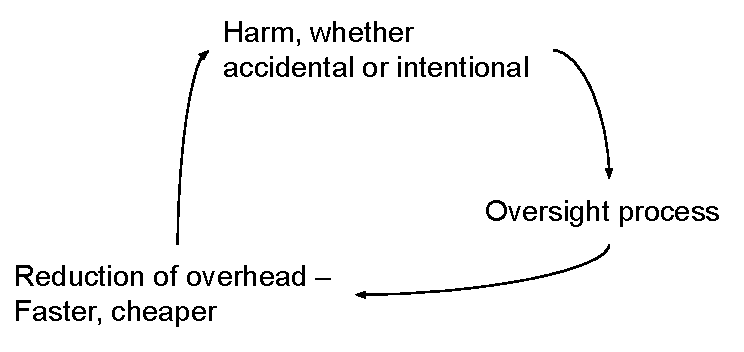
\includegraphics{images/process_loop_harm-oversight-improvement}
    \caption{loop: harm-oversight-improvement}
    \label{fig:harm-oversight-improvement}
\end{figure}


% https://graphthinking.blogspot.com/2021/04/laffer-curve-and-minimum-viable.html

\subsection{Processes as a tax on Productivity}

The Laffer curve is a claim in economics that there is a relation between government tax rates and the revenue from taxes collected. The relation, based on Rolle's theorem, says that between a tax rate of 0% and 100%, there must be some amount of tax that corresponds to the maximum of revenue. 

While the mathematical statement may be provable, the use in economics seems hand-wavy. In this post, I'll extend that hand-waviness to a different domain: bureaucratic processes in organizations. The relation to the Laffer curve is that bureaucratic processes a tax on productivity. 
    \subsection{Tactic: Approval, Forgiveness, Opposition}
% https://graphthinking.blogspot.com/2017/10/flipping-approval-mentatlity.html

A common task is consensus regarding action or expending resources. There are distinct options about how to get that consensus:
\begin{itemize}
    \item Seek approval. Incurs both providing justification and waiting.
    \item Ask forgiveness. Often viewed as being in contrast to seeking approval. 
    \item Solicit opposition. 
\end{itemize}
The best way to proceed depends on the personalities of the people involved in building consensus and their relationships. 

Most organization default to approval processes. Each new idea needs to be signed off as approved by a sequential list of bureaucrats. The sequence (not concurrent) process may be known in advance, or it may be ad hoc if the request is novel.

Relying on approval is harmful to innovation because sign-off by each bureaucrat is interpeted as ``I am 100\% in agreement with this.'' Each stakeholder has to bless innovation and tie their reputation to the outcome.

The ``I won't stop this'' is a more useful paradigm. With the consensus process language changed to "I won't stop this," then the bureaucrat can avoid taking responsibility for the idea and therefore are not tying their reputation to the result.

% https://news.ycombinator.com/item?id=15407757 % subsection
    \subsection{Static and Dynamic Process}

% https://graphthinking.blogspot.com/2017/04/static-versus-dynamic-processes.html

Change within an organization is to be expected since the external environment the organization exists in is not static. With that premise, why are static processes that are not robust to change created in the first place? Answer: so policy creators can point to an effort and avoid looking neglectful.

Creating robust processes that are dynamic takes more investment. First, the underlying process must be documented. What is expected to happen? Who are the stakeholders? This logic is what is fragile to change. Second, document assumptions used in the process. If the assumptions are invalidated, then the process is broken and needs to be discarded or at least revised. 

The problem is that even when the process is documented and assumptions enumerated, they may not be checked to see if revision is necessary. Measurements need to be periodically taken to see if the assumptions are still applicable. \href{https://en.wikipedia.org/wiki/Sunset_provision}{Sunset provisions} have a similar intent of forcing renewal. 

A more quantitative approach is to tie a process to a cost/benefit model. The benefit to implementing a process comes at some cost. If the assumptions of the process can be tied to a cost/benefit model, then we can determine whether the process is worth implementing. Periodic measurements are needed to update the cost/benefit model and determine whether the process is effective.

    \subsection{Bureaucratic Debt}

% https://graphthinking.blogspot.com/2017/09/bureaucratic-debt-and-what-to-do-about.html

\gls{bureaucratic debt} is the cost of work need to change a process caused by choosing an easy solution now instead of using a better approach that would take longer.

The purpose of defining this concept is to capture the unquantified work resulting from decisions.


decisions in a resource constrained environment (insufficient time, money, labor). Each decision made results in options that are not explored. Some of these missed opportunities are associated with short-term versus long-term trade-offs of costs.

These opportunity costs (what the organization doesn't do) alters which future decisions become available.

Getting information (measurement) and analysis are costly in terms of money, time, skill, and labor.

Once the concept of bureaucratic debt is recognized, the question is how to track it.

To document bureaucratic debt, we need to capture decisions as they are made:
\begin{itemize}
    \item what is the decision to be made?
    \item when the decision was identified?
    \item when the decision was made?
    \item who made the decision?
    \item what options were identified?
    \item which option was chosen?
    \item what that option was chosen over the other options
\end{itemize}
The purpose of documenting decisions is to enable both aversion to bad decisions and attraction to good decisions. Without documenting decisions, there is no transparency, accountability, or historical ability to track dependencies. 

The documentation of decisions needs to be disseminated to stakeholders. This should occur as promptly as possible. 

The scale of decision impact determines the level of documentation. "Do I choose pencil or pen?" incurs negligible bureaucratic debt; therefore the documentation needed is also negligible. Projecting impact of decisions is a subjective prediction. 

Similarities of technical debt and bureaucratic debt
In developing software, there are three artifacts: the software, documentation on how to use the software, and documentation on why to use the software. The two distinct types of documentation are typically combined in one document. Each of these three artifacts are independent. The ramification of this is that each artifact can be created independently, and it takes work to maintain synchronization of the artifacts. 

Similarly for a bureaucracy, there is the processes and policies which get applied to customers, the documentation of what those processes and policies are, and guidance on when the processes and policies should be applied. As with technical debt, these three aspects are independent. 
 %subsection
    \subsection{Design processes for Turnover of Staff}

% https://graphthinking.blogspot.com/2020/02/design-for-turnover-rather-than-rely-on.html

When designing a process, there are a few goals to optimize for: time-to-first-result, average latency, financial cost, flexibility to input conditions, scalability. 
    %% https://graphthinking.blogspot.com/2021/04/laffer-curve-and-minimum-viable.html

The Laffer curve is a claim in economics that there is a relation between government tax rates and the revenue from taxes collected. The relation, based on Rolle's theorem, says that between a tax rate of 0% and 100%, there must be some amount of tax that corresponds to the maximum of revenue. 

While the mathematical statement may be provable, the use in economics seems hand-wavy. In this post, I'll extend that hand-waviness to a different domain: bureaucratic processes in organizations. The relation to the Laffer curve is that bureaucratic processes a tax on productivity. 
  \newpage
  \section{Communication within a Bureaucracy}
  I don't want to talk specifically about paper memos versus email versus phone calls versus video chat versus Skype versus slack. 
The relevant attributes are synchronous versus asynchronous. Searchable or not searchable. In that context, there might be some interesting bureaucratic specific things to think about
    \subsection{Role of Communication within a Bureaucracy}

Communication facilitates delegation of work, allocation of resources, relationship creation/maintenance, and carrying out processes.


% https://graphthinking.blogspot.com/2021/09/why-is-everything-so-hard-in-large.html

Prisoner's dilemma says communication yields better outcomes.
Communication has a cost -- delay action, and opportunity costs


Coordination among participants is one way to break the \href{https://en.wikipedia.org/wiki/Prisoner\%27s\_dilemma}{Prisoner's dilemma} of unaligned incentives. In practice, communication takes times and skill; not everyone is willing to invest in communication that is seen as not ``doing the work". Additionally, accounting for the \\href{https://en.wikipedia.org/wiki/Allen\_curve}{Allen curve} takes effort. Lastly, the time needed to arrive through consensus at an optimal approach for a given situation may exceed time available for solving the problem.
 
    \subsection{Failure to communicate}


Role of assumptions 

How does communication among individuals fail?
"levels of enlightenment"
\begin{enumerate}
    \item I feel bad
    \item I can't do what I want
    \item I can't do what I want in the way I want
    \item There is a problem
    \item I have a solution
    \item I have an implementation
    \item I tried but my solution didn't work
    \item life sucks but I get a pay check
    \item I quit (in hopes of being more successful somewhere else)
\end{enumerate}

    \section{Communication Preferences}
% why this matters: source of friction among bureaucrats
% benefit to reader: understanding why people are different

There are typically multiple communication channels available between bureaucrats in an organization. Rather than focus on specific implementations using specific technologies, consider two variables. The first variable is asynchronous versus synchronous. Examples of asynchronous communication channels include voice mail, email, web forums, web sites, calendars. Synchronous options include phone calls, video calls, in-person, text-based chat like IRC or Slack. The distinction between these can be blurry, like if someone immediately replies to your (asynchronous) email.  The second variable is a set of categories: voice (e.g., phone), text (e.g., website, web forums, calendars), video (e.g., calls), and in-person. 

% https://graphthinking.blogspot.com/2016/04/communication-channel-equivalence.html
The lack of equivalence can be seen in comparing text with audio which has been converted to text. In addition to the text transcription, voice audio also has inflection, volume, volume variation, rate, rate variance.

The relevance to a bureaucrat of identifying these channels is to know which channel is preferred for what purpose. To be an effective bureaucrat there are reciprocal actions. First, you should list your own preferences so that people know how best to engage with you\marginpar{[Tag] Advice}. Second, you should learn and then leverage the preferences of individuals you collaborate with\marginpar{[Tag] Advice}.

As an example of knowing your own behaviors, do you keep your calendar up-to-date? Or is your calendar irrelevant? Is that preference stated explicitly to the people who might reference your calendar? Is your calendar visible to your coworkers?

Text chat is useful for asynchronous interrupts. Text chats are better than stopping by in person or calling on the phone since in-person drive-bys and phone calls interrupt whatever I'm thinking about or discussing. The purpose of the text chat is either a reminder or seeking a convenient time to talk. 

Email is useful for notifications or questions or setting up logistics. If I don't respond to a question or request for action within 2 days, please send a reminder. 

Video calls are my preferred method for group meetings. Group meetings via video call scheduled in advance on my calendar are best. Impromptu video calls are acceptable but as interruptive as a phone call. 

In-person discussions are my preferred method for one-on-one discussions. Stopping by my desk  without an appointment interrupts whatever I'm thinking about. If a calendar invitation is inconvenient, a text chat confirming my availability prior to the in-person discussion is helpful. 

Phone is useful when the caller is unable to be present in-person. Phone, being voice-only, is inferior to video calls. Unscheduled phone calls interrupt whatever I'm thinking about. I've intentionally disabled voicemail. 

Status updates in electronic issue trackers or wikis or forums are best (rather than email-only). Notifying in text chat or email that a wiki page or issue is updated is helpful but not mandatory. 

Given all those caveats, I prefer communication in any form at any time over surprises. 

If you're not sure whether you should communicate, default to communicating. If you're not sure whether communication would interrupt something, check my calendar and then communicate. If it's urgent or blocking progress, ignore my calendar. 

Know when to switch communication channels.\marginpar{[Tag] Advice} When to start in one channel and then escalate. Text to phone to in person 

    \section{Communication within a Bureaucracy}

\subsection{Communication is Critical for Bureaucracy}
\Gls{bureaucracy} is a system of distributed knowledge and distributed decision making. In that context, the importance of effective communication cannot be overstated. At the same time, writing and speaking are incomplete and imprecise. This is why iteration is critical when establishing a shared model.

Relationships matter for communication. 
\href{https://en.wikipedia.org/wiki/Metcalfe\%27s_law}{Metcalfe's law} says
\marginpar{[Tag] Folk wisdom}
the value of an organization is proportional to the square of the number of people interacting in the organization. Broadening your network of collaborations enables your effectiveness and that of your fellow bureaucrats. 

% https://graphthinking.blogspot.com/2018/08/confusion-leads-to-confusion.html
If you don't know what is happening in your organization, or you don't understand why certain decisions were made, your confusion could leave you focused on your own self interests since that is what you have some control over and insight on. This same analysis applies to each person in the bureaucratic organization. There is a way out of this harmful cycle: broadcast your intent to other people, be transparent with decisions, and share the results of your activities. That decreases the confusion other people may have about you, and if reciprocated can improve effectiveness. 

Feeling saturated with meetings, emails, phone calls, and other coordination may stem from ineffective communication. 
Communication that is incorrect, imprecise, redundant, and insufficient can be improved. 
% https://graphthinking.blogspot.com/2016/04/impact-of-communication-on-negotiation.html
Poor communication yields poor negotiation. Then the interaction defaults to an emotional struggle of will power. 

%*************************************
When a challenge that spans multiple bureaucrats (and may span teams) is recognized in a bureaucracy, a typical response is to hold more meetings (ok for decision making) and send more emails (ok for sharing information). Both these channels are ephemeral. Share information using channels that are discoverable and durable. 

%*************************************

In this book I don't address paper memos versus email versus phone calls versus video chat versus Skype versus Slack. 
The relevant attributes are agnostic to specific technologies and implementations: synchronous versus asynchronous; discoverable or not discoverable; searchable or not searchable. 
%In that context, there might be some interesting bureaucratic specific things to think about.

%*************************************

Communication within a bureaucratic organization occurs on a gradient of how official the information is. Examples of the gradient ordered from unofficial to official:
\begin{itemize}
    \item I just made this up and I have no authority
    \item Based on my experience, ...
    \item Based on my training, ...
    \item I heard from someone else (folklore from a peer)
    \item I heard from someone in a position of authority
    \item Referencing a written document
    \item Referencing a written document that looks official
    \item Referencing a written document that looks official with the signature of a position of authority
\end{itemize}
These indicators convey the relative importance of information for the bureaucrat. 

%*************************************
\ \\

Information within a bureaucracy shapes the relationships of bureaucrats. That spans from not sharing information (which can harm or protect relationships) to being transparent to being vulnerable.  
Being transparent conveys ``here's what is happening." Being vulnerable expands that to ``here's why that's happening or what might happen."

\ \\
    % https://graphthinking.blogspot.com/2020/05/invisible-bureaucracy.html

\subsection{Social and Bureaucratic interactions}

Interactions with other people in an organization are either social interaction or bureaucratic interaction. 

As examples of each of these,
\begin{itemize}
\item Social interaction example: "Did you see the game on TV last night? Our team really did well, right? I thought about getting tickets for the game but they were sold out."
\item Bureaucratic interaction example: "You'll need to get approval from Sue before presenting your idea to the board for their review. Then talk with Russ and get his thoughts."
\end{itemize}
Both social and bureaucratic interactions are vital to cohesion in an organization of people. 


Bureaucratic interaction can be broken into two subcategories: \gls{visible bureaucracy} (procedures and processes are written down and can be discovered by stakeholders)  and \gls{invisible bureaucracy} (procedures and processes are known to some stakeholders and are conveyed verbally to some of the other stakeholders).

Invisible bureaucracy is akin to invisible domestic or relation work outside the professional environment. The work associated with emotional cohesion, logistics, planning, scheduling, and communicating is hard to quantify so it does not get counted.

To make invisible work and invisible bureaucracy visible, document the work.


The relevance of this jargon is to break down the components of an organization's "culture" experienced by participants. The ratio of social/visible bureaucracy/invisible bureaucracy is a characterization of the culture. There are norms associated with each of these three categories. % subsection
    \subsection{Communication Tips}

The role of verbal communication is critical for bureaucrats. 
There is a lot of advice on effective communication (enunciate, speak loud enough to be heard, be humble, be curious), so the advice below is highlighted because of prevalence in bureaucratic organizations. 
The following is generic to interactions outside of bureaucracy. 

For general writing tips, see Strunk's and White's Elements of Style and other resources \footnote{\href{https://www.youtube.com/watch?v=vtIzMaLkCaM}{LEADERSHIP LAB: The Craft of Writing Effectively} and \href{https://www.youtube.com/watch?v=aFwVf5a3pZM}{LEADERSHIP LAB: Writing Beyond the Academy}}.

\subsubsection{Tip: Not all interaction challenges are communication problems.}
Sometimes an inability to discuss ideas is not a communication problem but a psychological deficit of personality. Distinguishing ``I'm an ineffective communicator'' from ``the person I'm talking with doesn't communicate effectively'' from ``that person has a diagnosed psychological reason they are unable to communicate'' is tough for those of us who are not psychologists or psychiatrists. 

%how to measure effectiveness: The waste or inefficiency in a bureaucracy is a measure of the lack of coordination or inconsistent decision making among the members

\subsubsection{Tip: Avoid relying on stereotypes.}
Within an organization different teams may build up reputations for certain behaviors, or there may be significant events that the team is associated with. 
When interacting with members of a team that has a reputation, avoid relying on that stereotype or event as an opening for discussion. 
You're speaking to an individual, so address that person's behavior.



\subsubsection{Tip: Avoid questions that have a binary response\label{sec:yes_no_questions}.}

Responding to a request with ``no'' is advantageous for the person replying to the question. There is less work required, less risk of failure, and better continuity. As an example of a poorly framed question, I could ask, ``Can I have a copy of the data you're using?'' The person I'm asking is less disrupted if they refuse to share. 

A more constructive phrasing is ``I need information on X to work on Y, and I think you have information about X. How can you help me get information on X?'' By clarifying my intent, I allow the person with the data to provide options I may not have considered.

Similarly, when I'm being asked for information, I try to learn the person's intent motivating the question. Sometimes the requester doesn't actually know what to ask for. Instead of ``no'' I try to figure out how to enable the person to be successful. 

\subsubsection{Tip: Leverage the other person's experience while focusing on your own\label{sec:advice}}

Advice without context is less effective.\\
\textit{Bad}: ``Here is what I think you should do in that situation.''\\
\textit{Better}: ``Here is what I did in that situation.''

People usually find talking about themselves an easy topic if you are curious about their experiences. 
If you can learn the other person's background and history and motivations, you can weave that into the advice you provide. 
Tailoring your message increases the likelihood of implementation. 

\subsubsection{Tip: Avoid Platitudes\label{sec:platitudes}.}
% https://graphthinking.blogspot.com/2017/10/why-platitudes-are-used.html
\href{https://en.wikipedia.org/wiki/Platitude}{Platitudes} are \gls{thought terminating}; the statement feels true and is resistant to debate. Platitudes capture a feeling with sufficient accuracy, but with imprecise language. As a result, there's no specific action.

Because platitudes result in a conclusion, the conversation participants may feel more bonded. However, that bond is shallow.

Example platitudes to avoid:
% https://graphthinking.blogspot.com/2017/02/phrases-which-serve-as-thinking-stoppers.html
% https://graphthinking.blogspot.com/2017/10/a-list-of-platitudes.html
\begin{itemize}
    \item pick your battles
    \item Some things you can't explain
    \item Your time will come.
    \item You can be anything that you want to be
    \item I just want to get through this day
    \item It is what it is
    \item I'm just one person
    \item That's that
    \item Life's not perfect
    \item Life's not fair
    \item There's only so much you can do about it
    \item What is meant to be will be
    \item It is God's will
    \item It's part of God's plan
\end{itemize}

If your goal is to understand a concept or issue deeply, you need to use precise language.

\subsubsection{Tip: Strive to use Precise Language}

Imprecise language causes miscommunication. Intent is unclear, as is expected consequence.

If you have a specific definition for a word central to the topic of interest, ask your new collaborator for their definition. Do not expect others to share your definition even when there are established norms for the topic. 

Instead of asking a collaborator, ``Are you taking action on this topic?'' ask ``What actions are you taking on this topic?''

If someone claims, ``We plan to get to that action,'' ask for a timeline. A deadline can be for an artifact or a re-evaluation of the topic.

In the short-term imprecise language takes less work to create and can take less time to convey. 

The importance of precise language is proportional to the potential consequences of action/inaction/wrong action.
Precision also should be proportional to the complexity of the topic being discussed. 

\subsubsection{Tip: Word is bond\label{sec:word-is-bond}}

Your communication (verbal, written) is your reputation. People rely on what you tell them even if there isn't legal recourse. Reliance on your word is why precision matters. 

Frustration and disappointment follow when you don't uphold your word, or others misinterpret your imprecise language, or you are misunderstood.

Communication implies responsibility for the content.  There is a corresponding accountability in the relationship between speaker and listener (or writer and reader).

\subsubsection{Tip: Take care near the boundaries of knowledge}

Trying to find someone else's extent of knowledge is tricky -- they don't want to appear stupid. They may interpret the exploration at a trap. ``I don't know'' can be an embarrassing statement to make, even if you don't share their embarrassment. 

Knowing the limitations of your own knowledge and disclosing those boundaries to others is critical. Distinguish what you know from speculation about things you don't. 

\subsubsection{Tip: Listen all the way to the last word of the speaker}

Formulating a response to the first part of an idea or a sentence is tempting. Waiting for the speaker to finish before thinking of how to response is courteous. Waiting creates a pause which makes you seem more thoughtful. 

This is complicated by the speakers who include long pauses for contemplation and then resume. 

\subsubsection{Tip: Eliminate speaking over other people.\label{sec:crosstalk}}
% https://graphthinking.blogspot.com/2017/10/crosstalk.html

Crosstalk occurs two people who are communicating verbally experience interference from another audible conversation. That can occur because a third person is talking at one of the original two participants, or when four or more people are holding two separate conversations concurrently. 

Crosstalk in a bureaucracy is motivated by
limited time available to communicate. A meeting participant may feel inspired by something someone else said and want to interject. 
%Typically manifests as popcorn style stories based on experience. 
%Intended as wisdom for self-validation by others in our community. 
Crosstalk can indicate engagement and enthusiasm, or it can be due to the speaker wanting to dominate the topic through interruption. The likelihood of crosstalk is dependent on the level of aggressiveness of participants.
In either case (enthusiasm or power-seeking), the original speakers are disrespected. The original speaker may feel annoyed at being interrupted.



%Crosstalk has four roles and a minimum of two people participating: the discussion facilitator, the original speaker, the interrupter, and other meeting participants. 
%During crosstalk, the discussion facilitator loses control of the interaction to the interrupter.  
The audience is frustrated by the lack of clarity of where to focus. This distraction causes participants to lose of focus and productivity of the interaction decreases.

Bystander intervention for out-of-control meeting: raise your hand. \marginpar{[Tag] Actionable Advice} This non-verbally reverts focus back to the discussion facilitator. 

\subsubsection{Tip: Account for Warnock's dilemma}
% https://graphthinking.blogspot.com/2018/09/dealing-with-warnocks-dilemma-in.html
\href{https://en.wikipedia.org/wiki/Warnock\%27s_dilemma}{Warnock's dilemma}
is the common experience of figuring out how to interpret not getting feedback. This is especially vital in meetings where the speaker or facilitator needs to gauge participant comprehension of delivered content. Simply asking ``Does anyone not understand what I just described?" is likely to get no response from attendees because individuals want to avoid looking stupid.

\ \\
\textit{Technique}: Pick an individual to provide a recap.\\
\textit{Technique}: Survey the audience using multiple choice to gauge understanding.\marginpar{[Tag] Actionable Advice}

\subsubsection{Tip: Seek action with a deadline}

% https://graphthinking.blogspot.com/2017/11/collected-wisdom.html
When asking someone for help or input, specify a deadline for their response. \marginpar{[Tag] Actionable Advice}This helps the person prioritize their tasks.

\subsubsection{Tip: Identify the cause of miscommunication}

% https://graphthinking.blogspot.com/2019/06/miscommunication-versus-inability-to.html
\begin{itemize}
    \item miscommunication the cause is often due to definitions of words used or differences in context. In this situation, additional time spent communicating and taking different approaches is sufficient to remedy the issue.
\item A speaker may be inarticulate. If the speaker is unable to coherently convey their internal experience to a listener, then the communication failure is of a distinct category. No amount of additional communication will lead to improved understanding on the part of the listener.
\item A speaker simply has nothing to say about a subject. Regardless of whether they are capable of articulating a concept, they may be unable to relate to the topic. Often a person in this situation still wants to participate, but they are unable to meaningfully contribute. 
\end{itemize}
% https://graphthinking.blogspot.com/2019/05/identifying-empty-talk.html
Empty talk is the use of words that are ill-defined, emotionally resonant, inactionable, and impersonal.

\subsubsection{Tip: ask-tell-ask}

Collaborating with fellow bureaucrats who have expertise in areas you do not requires extra work. There may be differences in the words used to describe certain situations, more precision in wording that you're used to, or thinking about situations in ways you are not familiar with. In that context, to bridge the differences you can ask, tell, ask\footnote{\href{https://cepc.ucsf.edu/sites/cepc.ucsf.edu/files/Curriculum_sample_14-0602.pdf}{``The 10 Building Blocks of Primary Care: `Ask Tell Ask' Sample Curriculum''} and \href{https://www.the-hospitalist.org/hospitalist/article/125126/qi-initiatives/ask-tell-ask-simple-technique-can-help-hospitalists}{Ask-Tell-Ask: Simple Technique}}. 

The first step is asking what the other person's perspective is on the topic. This helps establish the appropriate level of nuance is and can tell you how that person frames the issue. The second step is to tell the person what you want to say. The ``tell'' step should leverage what you learned from the first ``ask'' step. Use phrasing that is consistent with what you just learned from the other person. The third step is to ask the person what they heard from you. If they are unable to tell you, you may need to refine your delivery. To improve the likelihood of success keep the content in the second step short. 

The ask-tell-ask technique can be used iteratively in the same conversation, especially in discussion complex topics with a new collaborator. \marginpar{[Tag] Actionable Advice}Using ask-tell-ask takes long than just telling but increases the effectiveness of the communication. You also get to learn more about the other person's perspective. 


\subsubsection{Tip: Initial responsiveness and status updates}
In a bureaucracy requiring approval, or soliciting input, sometimes waiting can provide value to the person doing the waiting. The request may be overcome by events, or the person asking may remind which indicates priority.

\subsubsection{Tip: Make deadlines explicit}

Typically requests have two deadlines. The first deadline is when a response is sought. The second deadline is when a response is no longer useful.  

As an example, suppose I am inviting people to a meeting. I send the invitation 5 days prior to the meeting and I want to know who is able to attend by 3 days before the meeting. The second deadline is the time of the meeting. Replies after that second deadline do not help me understand who is going to attend. 

\subsubsection{Tip: Read each email/memo/report to determine the purpose }
% https://graphthinking.blogspot.com/2021/03/read-each-email-to-determine-purpose.html

\textit{Problematic behavior}: scan the text of a message, see if there is immediate action or response needed. If no action or response is needed, go to the next email. \\
 That does not work for emails that contain logistics associated with future events. 

Instead, consider possible intentions of the person writing the email. 

\textbf{Decision needed}. Typically includes context. \\
\textit{Action}: if the team maintains a decision log, update that.
Response is selection of a choice.

Tip: Instead of asking for a decision, ask for if the person is opposed.

Tip: instead of asking for a decision, ask for the go-ahead. This framing biases the respondent towards action (specifically approval) rather than thinking. 

\textbf{Situational awareness}.\\
\textit{Action}: Expected default is no action, but interject if there's an issue.


\textbf{Action or Tasking}.\\
\textit{Action}: Do something within some deadline

\textbf{Approval sought}.\\
\textit{Action}: Confirm or deny

\textbf{Feedback sought}.\\
\textit{Action}: Assessment of proposal


\textbf{Meeting logistics}. Can be an announcement (widely available), registration (limited attendance), or invitation (specific to you). Attendance is optional or require. \\
\textit{Action}: Create or update a calendar event
Response should restate the logistics (time/date/location/purpose) to confirm. 

\textbf{Brainstorming}\\
May provoke a response for building on an idea.
``For your situational awareness, no action needed." Notification of activity by someone else. Or change in plans. 
If needed, a correction to the described direction might trigger a response or even a meeting.

\textbf{Reference} e.g. describing a process or business workflow. Or a citation.\\
\textit{Action}: Copy process documentation to wiki. Copy citation to bibliography.
Acknowledgement response thanking the sender for the update/clarification.

\textbf{Setting a formal policy or issuing an informal edict}\\
\textit{Action}: move the policy/edict documentation to Confluence or Wiki
Acknowledgement response needed only if the edit is aimed at just me or the group I am leading

\textbf{Question}\\
If this is a recurring question, move to a ``Frequently Asked Questions" page on Confluence or Wiki.
Response needed that provides answer or seeks clarification.


Here I'm using ``action" to refer to activities outside the email channel. 

If I read email to figure out the purpose of the email, that will help me determine what action and response are relevant. 

Whether I am the only recipient or on of many receivers can change the intent of the email, and whether I'm in the ``to" or ``cc" field matters. Unfortunately, ``to" versus ``cc" are not reliable indicators since email senders do not reliably conform to the expected use. 



%This categorization of text within emails is a useful natural language processing challenge for machine learning. Currently a few email providers already do some of this with identifying meeting logistics, providing reminders to follow-up, and providing reply snippets. A browser plug-in that differentiates the various purposes of text could help readers determine relevant actions and responses. 

An email sent to multiple recipients may have different purposes for different readers. The reader's role or knowledge may factor into how they interpret the content. The inclusion or exclusion of recipients alters how the content is understood. 

\subsubsection{Tip: Don't seek attribution for contributions; credit others\label{sec:credit-others}}

Give credit to others for good ideas and beneficial actions. Either they accept credit and you are seen as a contributor to their success, or they push back and you look generous. Credit is not a \href{https://en.wikipedia.org/wiki/Zero-sum_game}{zero sum game}.

\subsubsection{Tip: Offer to take blame\label{sec:take-blame}}

Before an action commences, tell collaborators that you are willing to accept blame if something goes wrong. This alleviates their fear of risks.

\subsubsection{Tip: Survey stakeholders}
% https://graphthinking.blogspot.com/2016/01/how-to-solve-and-not-solve-problems.html

Suppose you are a \href{http://www.peacecorps.gov/}{Peace Corps} worker in Africa. You show up and the village doesn't have easy access to clean water. Villagers walk a long ways in dangerous areas for dirty, unsafe water. This is a very obvious problem and all the villagers agree that they don't have good water and that this problem should be fixed.

Implementing the solution would take about a week - get the equipment to the village, drill a well, build a pump.

You could take additional time and involve the villagers in this project. They could participate in getting the equipment, which should lead to a sense of ownership.
But then when the equipment shows up, they don't take action to drill the well. If the well is drilled, it soon falls into disrepair and the villagers are back to doing things they way they used to. What happened?

The villagers don't see access to clean water as the most significant issue. You came in and imposed your view of what the problem is and how to fix it. When you impose your view of what the problem is, the solution won't be adopted by villagers because they don't prioritize it.
It is better to survey the community to see how they operate. What do they think the problems are?
Both leadership and the community members need to provide priorities.

This issue is exacerbated if you come to the village as a representative of a company providing wells. You are biased when you ask, ``Do you have any problems?"

Of course the villagers have water problems which could be fixed with better wells. However, when you get into the details of placing or improving a well, they lose interest. What the community really wants is free installation, zero maintenance, easy to use, and no operational costs. That would improve their life.

When you say there's cost (both initial investment of capital and then operations/maintenance) and a learning curve associated with the solution, then the user's interest wanes -- you are presenting another cost/benefit ratio for them to evaluate. Then they ask ``Can we get by without the well?" Yes, they don't need the well -- they've survived without it.

Novel solutions (in this example, drilling a well and installing a pump) have have barriers to adoption. Two barriers are the current priorities of the community and the incumbent solution/processes.

If there are problems with higher priority, the community will delay implementing your solution. That's fine if the higher-ranked priorities are bounded, but they are often not. An example of this is the following:
Suppose a person has three tasks, and you introduce a solution which is a fourth task.
If the first task is ``go from point A to point B," then that task will eventually be eliminated and there will be three remaining.
If the second task is ``secure your village," that is an unbounded task. The person won't get to or won't prioritize your low-ranked task.

How will your solution impact their higher-ranked priorities?

\ \\

\textbf{Summary of what action should be carried out} \\

As the outsider, you should help the community enumerate and document all of the problems they identify. Then you can help enumerate and document how the problems are related (dependencies). Only then can you help the community identify and document the root causes.

If the solution you, the outsider, identified really is the root cause, then the community will arrive at that independently. If that is the case, then you can enable them to implement a solution which addresses the root causes. The community will then have a sense of ownership.
 % subsection 
    \subsection{Friction between teams within an organization}
An organization has finite staffing, money, time. Therefore, teams within the organization face a zero-sum distribution of resources.

When attempting to resolve friction between teams, there is an authority common to the teams, but that person lacks the nuanced insight, doesn't have time to get involved in every challenge, and doesn't want to micromanage multiple teams.

    %There are many books on how to do meetings well. 
    % How is this section (in a book about bureaucracy) distinct?
    % how does understanding bureaucracy matter in the context of a meeting? what's the change in behavior for the effective bureaucrat?
    Stakeholders care about the outcome of a decision. 
    In some sense, every participant in an organization is invested the outcome of every decision made because there is consequence to how resources are allocated and the direction of the organization. Every org member has an opinion, even lacking experience or expertise. 
    
    \subsection{Well-run meeting\label{well-run_meeting}}

Identify essential attendees. If someone does not need to be present, notify them in advance that you will share the meeting notes afterwards. 


Bad: no meeting agenda\\
Good: agenda\\
Better: agenda share with other participants
For formal meetings, share agenda in writing prior to meeting. 

TODO: Why an agenda matters in a bureaucracy: 

TODO: forces conspiring against agendas


For formal in-person meetings, Verify meeting venue has sufficient space, seating, working IT equipment

For formal virtual meetings, ensure participants are familiar with virtual meeting controls

TODO: why logistics/infrastructure matter in a bureaucracy:

TODO: forces conspiring against logistics/infrastructure
    \subsection{Characterizing Meetings}
% relevance of this section:
Characterizing meetings is critical to distinguishing which norms are applicable, and what people expect from the different formats. 

types of meetings: internal meetings, customer meetings, conferences, scheduled one-on-ones, impromptu walk-around,  

% https://graphthinking.blogspot.com/2019/12/what-is-purpose-of-this-meeting.html
Many purpose to a meeting
\begin{itemize}
    \item To gather input from attendees
    \item To make a pronouncement to attendees
    \item To educate
    \item To brainstorm ideas
    \item To make progress towards an objective
\end{itemize}
When the purpose is not explicitly stated, confusion arises.

When multiple purposes occur in one meeting and the transition is not explicitly stated, confusion arises.
The reason for this confusion is that the assumptions and expectations and norms of each purpose are different. When the attendees don't know the purpose or the purpose shifts, the behaviors and roles are in question.

% https://graphthinking.blogspot.com/2014/12/how-to-understand-meetings-at-work.html
Level of formality, start time (early | on time | late), 
end time (early | on time | late), utility, 
duration, number of attendees, number of speakers, number of participants.


What is the purpose of a meeting?

meetings involve people, either known or strangers
meetings involve information, either relevant or irrelevant. Relevant information is either new or related to previous work
meetings either have a leader or no leader (brainstorming). If there's a leader, the leader may be disseminating info to participants, or gathering information from attendees
%    \section{Make Effective Presentations\label{sec:presentations}}

% https://graphthinking.blogspot.com/2011/10/presentation-notes.html

By paying attention to a bad presentation, you can find problems that you do not want to repeat.

Speaking is vital at decision points in your career progress - at interviews, competitions, gaining new collaborators at conferences, impressing peers/boss/subordinates. Thus, it's best not to make these mistakes in those situations.

Aspects to a presentation
\begin{itemize}
    \item speaker: appearance, verbal accent, enunciation, smell
    \item slides: layout, content
    \item audience: background
    \item venue: size, technology available, lighting
    \item lead time: how much time do you have to prepare?
\end{itemize}
The following list is meant to be reviewed as a checklist.

Planning your presentation

In introducing your research, there are a few ways to open the talk
\begin{itemize}
    \item compliment the audience
    \item humor: relevant joke
    \item how does this work make me feel
    \item explain context and relevance in terms of money, number of people involved, size of system
\end{itemize}
Estimate the experience/education background of your audience prior to creating the presentation. The question being answered in the presentation is independent of audience, but the level of delivery depends on audience background.


Speaking to an audience outside your field:
\begin{itemize}
    \item Use jargon your audience is familiar with. For example, a physicist uses "quantization of energy" whereas an audience of mathematicians may be more comfortable with "discrete energy levels."
    \item Look for commonality. For example, both physicists and mathematicians use assumptions and build models.
\end{itemize}
Visual presentation:
\begin{itemize}
    \item Switching between dark and light slides in a dark room stresses the eyes (need time to adjust to varying light levels)
    \item In figures, use both color contrast and distinct symbols, in order to deal with colorblind audiences. See also http://jfly.iam.u-tokyo.ac.jp/color/
    \item making slides appear "professional" means adding non-informational content. This added content should be consistent, not distracting
\end{itemize}
Software:
Common choices include Latex (beamer), Microsoft Powerpoint. Less well-known are Prezi (and its open source equivalent, InkScape+Sozi add-on).

If you use Microsoft Word, a document PDF, notepad, or any other non-presentation software to make a presentation, then you are sending a few messages to your audience:
The audience isn't worth your time needed to develop or learn a proper presentation. 
You are not technically savvy.

Presenting multiple topics within one presentation:
Disparate topics require a segue to show why you are transitioning
Inter-relate the multiple topics 
Dealing with technical failure
If you plan to give a live demo, have screenshots of the process in the presentation. That way, if the demo fails you can show what was supposed to happen in the slides. If the demo works, skip the slides.
If possible, use the setup as close to reality as possible for practice sessions. Project onto the screen using the projector. This will show if the color contrast is sufficient.

Prior to giving a talk at a remote (or unfamiliar) environment

Questions to ask your host:

Will I have a projector and screen for the presentation?

If Power point available, what version is in use?

Will I be allowed to bring a USB drive and/or laptop into the location (security restrictions), or should I email the pptx file to you?

Day of talk

Appearance (suit and tie or jeans and t-shirt?):
\begin{itemize}
    \item under-dressed = I don't respect the audience
    \item overdressed = I'm better than you
    \item similar level of dress = I'm a peer
\end{itemize}
Some of these suggestions may seem glaringly obvious. The reason they are here is because I have personally seen them in "official" presentations given by a "professional"
\begin{itemize}
    \item Do not curse (profanity while speaking, or in the slide presentation, or even the name of the file)
    \item Practice the presentation (out loud in real time) at least once
    \item Run spell check before presenting
    \item Translate your slides from your native language to the language of your audience
    \item Tell a coherent story with a unified theme. Each slide should be logically connected to the following slide. Don't just put a bunch of slides with data together. You risk disorienting your audience.
\end{itemize}
Before the talk begins
\begin{itemize}
    \item Make sure your facility has power, a screen, a projector, pointer, any other necessary equipment. [Your host may not think of these things for you.]
    \item Make sure all equipment works and functions together
    \item Before the presentation begins, use a slide to make announcements and reminders:
\begin{itemize}
    \item list agenda if there are multiple speakers
    \item time talk begins, how long it will last
    \item Reminder: Turn OFF Cell Phones
\end{itemize}
    \item Announce whether to ask questions during talk (interrupt) or to hold questions until done
\end{itemize}
During the talk
\begin{itemize}
    \item Opening: Thank hosts/inviters/organizers. Establish a connection between you (the speaker) and the audience.
    \item Do not pace
    \item Do not stand frozen
    \item If you are the only person laughing at your joke, it isn't funny
\end{itemize}
 
After the talk
\begin{itemize}
    \item Let the person asking the question finish
    \item Restate the question to ensure the audience heard it and that you understood it
    \item Give the minimal answer. Save the long answer for followup
\end{itemize}

    % how to engage your audience
    % stages of dysfunction
%    % https://graphthinking.blogspot.com/2021/02/organizations-value-things-more-than.html
In large organizations, there can be significant bureaucracy associated with even small purchases. A multi-step review process may be incurred for a \$2000 acquisition.

Another measurement of value is that if an employee were to steal even \$200 worth of materials, the organization would likely punish that employee.


Those metrics apply to tangible goods, but not to people's time. Consider a meeting of 10 people and each person's cost is \$200 per hour. A wasted meeting is not unusual and certainly would not incur bureaucratic review processes. The cost to the organization is fiscally the same -- \$2000. Similarly, consider an employee who is late and causes a loss of productivity. Merely depriving the organization of \$200 worth of time is not punished in the same way theft is.

In fact, organizations default to meetings (even recurring meetings) rather than not meet. And being late to a meeting is accepted. 

We can debate the differences between theft of materials and theft of time. The financial argument is clear. 

Source: Andy Grove in "High Output Management"
    
    \subsection{One-on-one check-in meetings}

% https://graphthinking.blogspot.com/2021/05/the-agenda-for-one-on-one-meeting.html

One-on-one meeting questions for helping the manager understand the team member's status.
\begin{itemize}
    \item what are the objectives for the team?
    \item what have you been successful with since we last met?
    \item what is blocking our team's progress?
    \item what are your plans?
    \item how are you collaborating with the rest of the team?
\end{itemize}

Reflective prompts for one-on-one meetings:
\begin{itemize}
    \item If there was just one thing you could change about our organization, what would it be and why?
    \item How do you plan to train your coworkers on topics you understand and they don't?
    \item What have you learned in the past month?
    \item What are the biggest risks for the team?
    \item What's limiting your productivity?
\end{itemize}
Responding to these questions takes time (an hour) and willingness to be open. 

\ \\

The one-on-one check-in should be tailored to the phase of the employee's progression. 
\begin{itemize}
    \item new team member, either new to the team or new to the company. Here the focus of the one-on-one is to ensure a smooth on-boarding process. Does the employee have the necessary computer log-in accounts? Do they have an email account? Are they on the mailing list?\\
\textit{The duration of this phase could last between a day and two weeks.}
    \item team member is responsible for small tasks: the one-one-one is for discussions on training and sprint planning and sprint-reviews. Characterized by the team member being dependent on others for their success. In this phase the employee collaborates on tasks.
\textit{The duration of this phase could last a few months to years.}
    \item team member is responsible for large tasks (which get broken into subtasks): the one-on-one is to help the team member define their success. Activities include planning, resource allocation, assessment. Characterized by the need to coordinate with others on the team or other teams.
\textit{The duration of this phase could could be the rest of a career.}
    \item facilitating the productivity of others: rather than being task-oriented, this team member supports coworkers. 
    \item peer check-in: this one-on-one is a form of mentorship. The value of the exchange is to get a different perspective and to hold each other accountable.
\end{itemize}

TODO: How does the team member and the supervisor know when the next phase is appropriate?

TODO: What are the thresholds for change?

\ \\

https://news.ycombinator.com/item?id=30152268

\ \\

https://news.ycombinator.com/item?id=22341138
https://github.com/VGraupera/1on1-questions


%    \subsection{How to be a Successful Conference Attendee}

% https://graphthinking.blogspot.com/2012/02/how-to-succeed-as-attendee-at.html

\textbf{Before the conference}\\

Determine the date of the conference. Does it conflict with other events in your schedule?

How will attending the conference benefit your progress? Social interaction, presenting your ideas.

Submit your abstract for review prior to the deadline.

Apply for travel grant funding as needed. Look to the sponsoring organization, conference website, and your own host institution.

Find housing nearby the conference location. Find a roommate.

Book a flight/transportation. Plan to arrive at least a day before you are scheduled to speak. (Speaking on the day you arrive is tiring.) Flights on Monday and Friday are often more expensive than mid week. Cheapest flights are released on Tuesday. [link]

Coordinate someone to cover for you while you are gone.

Find out who else is attending the conference. Which talks look interesting. If there are people you know, let them know you are coming and would like to see them.

Start stalking attendee profiles. If it is a small conference/summer school, get a list of attendees and learn their names/interests.

Bring printed papers, CV, business cards. Distribute these at the career fair, your talk. Bring an night shade and ear plugs. Your roommate may snore.

\textbf{How to determine which sessions to attend}\\

For very large conferences (APS March meeting, Supercomputing), there will be a lot of content outside your field. This means if you go to short talks, they will be hard to understand since they are very focused. Therefore attend the invited and plenary talks (usually at the beginning of the week) even if they are outside your field. They will be at a more accessible level, helping to determine which subfields may be of interest.

Start socializing on the plane, in the airport. This is warmup for the conference.

\textbf{Upon arrival}\\

Register. Get map, current conference schedule.

Socialize as much as possible. This is the point of a conference. Talk to people in line, before and after talks, at meals, at the hotel. Advantages over a regular stranger are that (1) there is a common topic to discuss (other than the weather), (2) they are probably also interested in that common topic. Also discuss meta-topics -- how the talk went visually/audio, how the conference is being run. Both parties are probably out of their home environment/city, so that is another commonality.


Keep all receipts for purchases. Keep your airline boarding passes.

Write down interesting ideas that are triggered by conversations outside your specialty.


\textbf{After your return}\\

Send emails to people you spoke with/got business cards. "Thanks for talking with me about X at the Y conference last week."
For recruiters, "Thanks for talking with me about positions X at the Y conference last week. Attached is a copy of my curriculum vitae. Please contact me to schedule an interview."
%    \subsection{How to be a Successful Conference Organizer}

% https://graphthinking.blogspot.com/2011/11/how-to-organize-conference.html

Plan to fail: When X fails, what is the backup?


Checklist for before the conference starts
\begin{itemize}
    \item determine theme
    \item check that dates do not conflict
    \item recruit speakers (experts in the field).
Determine keynote speaker
\item menu plan. 
Vegetarian and non-veg items (account for dietary restrictions)
\end{itemize}




Relevant parties:
\begin{itemize}
    \item participants. Attending to learn from the talks. What are current standards, what are the new developments?
    \begin{itemize}
        \item paying to attend, or receiving funding to attend. 
        \item special: session host
    \end{itemize}
    \item speakers. Giving talk to increase prestige, broadcast learned knowledge. Educate others.
    \begin{itemize}
        \item Volunteer or speaking pay. 
        \item special: keynote speaker
    \end{itemize}
    \item vendors. Advertise and sell product, gain new users, interact with existing customers. Pay for attendance, booth space. May get advertising space in program, on website.
    \item logistical support staff. Invisibly ensure a smooth conference. 
Paid or volunteer
\end{itemize}


location of conference

conference = attendees are also presenters

summer school = attendees and experts are distinct

Maximum daily schedule:
Wake, learn, coffee, learn, lunch, learn, snack, learn, supper

\textbf{Before the conference}\\

Scheduling the conference
Does the conference date conflict with the schedule for the audience? School, holidays, other conferences.

Finding good speakers
Need smart people who make good presentations on relavent topics.

Advertise
\begin{itemize}
\item Facebook group
\item Facebook event
\item Twitter updates
\item Youtube previews
\item Conference website
    \begin{itemize}
      \item Schedule of speakers, location of events
    \item Where to book hotel
    \item Transportation to/from conference (local bus or taxi)
    \end{itemize}
\end{itemize}
Minimum facilities
\begin{itemize}
\item bathrooms
\item presentation area
\item snack/conversation area
\item registration
\item speaker preparation/rest room
\end{itemize}

Catering must be professional. Must include liquids, especially coffee and at least one alter-
native.

Audio/Visual (AV) setup
for an audience of more than 20, a microphone is needed
Have a backup projector ready
Power standards
If participants will be using equipment from a country with a different electrical standard, be sure converters are available. Instead of each person using their own converter, use one converter and an outlet strip.


specify rules for the badge explicitly by printing them and including them with the badge
\begin{itemize}
\item badge is non-transferable
\item badge must be visible at all times
\item photo identification required upon request
\item tampering with badge invalidates usage
\item cost for badge replacement is \$XX
\end{itemize}
Other rules:
\begin{itemize}
\item all seating is first-come, first serve basis
\item no refunds
\item failure to comply with staff and security directions will result in badge revocation
\end{itemize}
offer coat check if weather is cold



Before participants arrive
Test wireless internet connection. Know the Network Administrator
Send an email with the following information
website for conference
transportation from airport to conference location
expected temperature range and weather type
dress style (business casual, formal)
If tutorials require computation, minimize dependence on remote computers. Network will be flaky, remote computer will be overwhelmed.

When participants arrive
Name tag, map, printed schedule

During the conference

Basics:
any medical problems must be addressed immediately. Health and safety of participants is primary concern
everyone getting food, sleep


For each presentation
Have water available for the speaker near the podium
Each speaker needs to have host. The host cuts off the speaker at the appropriate time. Otherwise the audience and next speaker are screwed by the overage. Experts like to talk about their work.

Increasing interaction
\begin{itemize}
    \item Informal coffee breaks. Allows for existing contacts to improve
    \item Each participant gives an "elevator talk." 1 minute, 1 slide (or with nothing).
    \item "Speed dating:" one-on-one interaction. Trade elevator speeches and business cards.
    \item "Think, pair, share." Give participants a scenario or question to think about. Then break into small groups (2 to 5) to discuss the topic. Finally, have groups share their results with other groups. Sets of groups can have different topic. For example, 30 people split into groups of 5, with three scenarios to discuss (two groups per scenario). If a problem is able to be broken into 3 parts (i.e., theory, experiment, marketing), then each set of two groups can work on a different part.
    \item If meals are included in the conference, force mingling among different social cliques. Instead of different disciplines at different tables, group people (assigned seating) by favorite color. See Birds of a feather
\end{itemize}

After the conference
Post presentations, conference materials online

Send thank you notes to everyone who helped
\begin{itemize}
    \item hotel/convention center
    \item attendees
    \item presenters
    \item organizing and support staff
\end{itemize}
Send surveys speakers and to audience to gauge success


prepare report to funding agency

\chapter{Last chapter}


Learning bureaucracy as a skill doesn't mean you can ignore personalities of individuals. Bureaucracy as a skill is in addition to being a good person, being an effective member of a team, being a good project manager, having technical skills, etc. 

% If bureaucracy is a distributed knowledge distributed decision system, compare with paxos and Byzantine generals
% https://en.wikipedia.org/wiki/Paxos_(computer_science)
%https://blog.the-pans.com/understanding-paxos/
%https://martinfowler.com/articles/patterns-of-distributed-systems/paxos.html

% https://en.wikipedia.org/wiki/Complexity_theory_and_organizations


\appendix

\chapter{Assessments for Publication}
\chapter{Reader's Report\label{sec:reader_report}}
An view from inside bureaucracy as a \href{https://en.wikipedia.org/wiki/Complexity_theory_and_organizations}{complex adaptive system}. 

Central claims:
\begin{itemize}
    \item Everyone in modern society participates in bureaucracy. Therefore becoming skilled is useful.
    \item Individuals already have experience with bureaucracy from conventional roles in modern society. 
    \item Bureaucracy requires 
    \begin{itemize}
        \item sufficient scale because it is an emergent phenomenon for distributed knowledge and distributed decision making. 
        \item lack of common quantitative feedback mechanism for individuals.
    \end{itemize}
    \item The techniques of bureaucracy are what lead to emergence at scale: meetings, processes, communication. 
\end{itemize}
The consequence of thinking like a bureaucrat is that
\begin{itemize}
    \item you are not limited to only the direct personal interactions that you have with other people. Framing allows you to think about processes that exceed your direct visibility and experience
    \item Help you recognize options beyond the naive defaults associated with fallacies (\ref{sec:fallacies}). What's feasible? What's negotiable?
    \item Decrease surprise when thing is not the way you naively expect. Name dilemmas, trilemmas (\ref{sec:dilemma_trilemma}), known hazards (\ref{sec:unavoidable_hazards}).
\end{itemize}
\newpage % section
\section{Audience Analysis}

Primary audience for this book is self-identified novice bureaucrats and people planning to work in a bureaucracy. Value of this book is advice beyond ``be a good person'' and specific to the role of a bureaucrat (and not project manager/team lead/software developer). 

Secondary audience is white collar workers who have experience working in a bureaucracy and are just realizing they are bureaucrats. This audience will find some of the information to be already known. 

Tertiary audience is non-bureaucrats who want to better understand why bureaucratic systems are challenging. This book won't be a popular best seller, but it is intended for a lay audience and does not assume prior academic exposure to the topic.

Lastly, researchers of bureaucracy. This book is not a theoretical systemic analysis. \newpage  % section

\chapter{Book notes}
\section{``Dynamics of Bureaucracy'' by Blau}

\cite{1955_Blau}

Intended audience:

Ben Payne has read this book: in progress\\
Ben Payne has a copy: yes\\
Ben Payne's assessment:

\newpage
\section{``Values of Bureaucracy'' by Du~Gay\label{review:dugay_values}}

\cite{2005_DuGay}

Intended audience:

Ben Payne has read this book: no\\
Ben Payne has a copy: yes, electronic\\
Ben Payne's assessment:


Each chapter is from a workshop on ``Defending
Bureaucracy'' held in 2003. Each chapter has a different author. \newpage
\section{``Handbook of Bureaucracy'' by Farazmand\label{review:farazmand_handbook}}

\cite{1994_Farazmand}

Intended audience:

Ben Payne has read this book: no\\
Ben Payne has a copy: no\\
Ben Payne's assessment:


\begin{quote}
    This encyclopedic reference/text provides an analysis of the basic issues and major aspects of bureaucracy, bureaucratic politics and administrative theory, public policy, and public administration in historical and contemporary perspectives. Examining theoretical, philosophical, and empirical interpretations, as well as the intricate position of bureaucracy in government, politics, national development, international relations, and a host of other institutions, the book focuses on the multifunctional role of public bureaucracies in societies with various socioeconomic, political, cultural, and ideological orientations and covers a wide range of processes and subjects.\footnote{\href{https://www.routledge.com/Handbook-of-Bureaucracy/Farazmand/p/book/9780824791827}{https://www.routledge.com/Handbook-of-Bureaucracy/Farazmand/p/book/9780824791827}}
\end{quote}\newpage
\section{``Utopia of Rules'' by Graeber\label{review:graeber_utopia}}

\cite{2015_Graeber}

review: https://muse.jhu.edu/article/749032/pdf

review: https://journals.sagepub.com/doi/abs/10.1177/0170840615590746?journalCode=ossa

% https://www.amazon.com/gp/product/1612195180

Intended audience:

Ben Payne has read this book: no\\
Ben Payne has a copy: yes, electronic\\
Ben Payne's assessment: written by an anthropologist; gives an outsider's view and the experiences of a subject of bureaucrats. Introduction gives a good history of modern bureaucracy.


This book is comprised of an introduction, three chapters, and an Appendix. 

In the introduction Graeber proposes his ``Iron Law of Liberalism'',
\begin{quote}
    any market reform, any government initiative intended to reduce red tape and promote market forces will have the ultimate effect of increasing the total number of regulations, the total amount of paperwork, and the total number of bureaucrats the government employs.
\end{quote}

Graeber claims working-class Americans see government as comprised of politicians and bureaucrats.

The options for decision making are bureaucracy and the market.


First essay starts with an illustration of the maze.\newpage
\section{``Research Handbook on Street-Level Bureaucracy'' by Hupe\label{review:hupe_handbook}}
\cite{2019_Hupe}


Intended audience is researchers.

author has read this book: no\\
author has a copy: no\\
author's assessment:

\begin{quote}
Street-level bureaucracy concerns a vital part of the ways in which public policy programs are implemented, particularly through the relationship between public officials and individual citizens. Addressing the state of the art and providing a systematic exploration of the theoretical and methodological issues at stake, this Research Handbook is a crucial contribution to the analysis of public policy from the perspective of the ground floor of government. 

The Research Handbook covers theoretical themes in current research such as institutional theory, social inequality, national culture, discrimination and representation, digitalization, and accountability. Analysing the role of teachers, police officers and other street-level bureaucrats, chapters explore how these individuals implement policies through their daily contact with citizens. Further sections investigate the methodological tools for research, as well as the future challenges facing the area. Peter Hupe concludes with lessons for the study of street-level bureaucracy and a significant research agenda for the topic.\footnote{\href{https://www.ippapublicpolicy.org/book/research-handbook-on-street-level-bureaucracy/19}{https://www.ippapublicpolicy.org/book/research-handbook-on-street-level-bureaucracy/19}}
\end{quote}\newpage
\section{``Street-Level Bureaucracy'' by Lipsky\label{review:lipsky_street}}

\cite{1983_Lipsky}

Intended audience:

author has read this book: yes\\
author has a copy: yes, physical\\
author's assessment:


pages 192 to the end.

Roles: customer, bureaucrat, boss of the bureaucrat

% https://graphthinking.blogspot.com/2018/08/how-to-decrease-bureacracy.html
In isolation, none of these ideas should be surprising.
\begin{itemize}
    \item automate recurring decision processes. This decreases bureaucracy by removing subjective influence of bureaucrats
\item where automation is infeasible, make customer advocates with end-to-end authority available
This decreases bureaucracy by improving customer's navigation of processes
\item make processes transparent to participants
This decreases bureaucracy by improving customer's understanding of processes
\item make information discoverable (e.g., via search engine) 
This decreases bureaucracy by 
\item make information directly available, rather than mediated by a person
\item after an interaction is completed, summarize the steps and outcome for the participant
\item when a process fails the needs of a participant, investigate the failure and improve the process
\item make the goals and priorities of the organization clear to all
\item define measurable standards of performance, both for individuals and teams
\item train bureaucrats how to engage participants effectively; these interactions determine the culture
\item train bureaucrats by addressing their immediate problems (e.g., through mentorship)
\item make employment desirable to people who have desirable characteristics (e.g., educated candidates)
\item enhance accountability to peers (e.g., peer review of actions and outcomes)
\item ensure that incentives for organizations and individuals encourage improvement rather than maintenance of status quo
\item decision making should be pushed down the hierarchy to the practitioner
\item when decision making requires cross-organization interaction, form a team of practitioners
\item bosses should share workload with their team in order to gain practical exposure to current challenges
\item seek feedback from process participants; then provide status updates on the implementation process
\end{itemize}
\newpage
\section{``Bureaucrat's Handbook'' by O'Hearn\label{review:ohearn_handbook}}

\cite{2015_OHearn}

Intended audience: novice bureaucrats starts their public service career

Ben Payne has read this book: yes\\
Ben Payne has a copy: yes, physical\\
Ben Payne's assessment: terrible; avoid this book!


As a government bureaucrat, I wanted to see if this book could be useful for helping new members of my organization. This book is not appropriate for that use, and the book contains bad advice. Some of the views are harmful. 



In a paragraph about communicating with the public on page 51, the author provides a racist observation: "If the person you are talking to is Asian, and they are nodding when they say yes, assume they don't have the slightest idea of what you're saying, but are too polite to tell you."



In the chapter on education, on page 12 the author's advice is, "To be a good bureaucrat you should become computer literate, as opposed to becoming computer stupid. This is true for any career field you choose. Almost all job applications are submitted on the computer. Office E-Mails have replaced typed memorandums." 



This book was published in 2015, so this content is jarring from the perspective of 2022. I suspect part of the cause is that author is old; the author bio mentions a 48 year career, which means he was probably 70 at the time of publication. 



Setting aside the bad advice and harm in this book, the author's view is that a bureaucrat is a government employee. The author advocates working in Human Resources or a budget office since those are stable jobs. The book does contain some valid observations about life as a bureaucrat; however, the valid insights are outweighed by the number and importance of incorrect explanations. 



The book appears to based wholly on the author's experience. No citations to research and no surveys are mentioned. Only two other publications are cited (Webster's dictionary for definitions, and the book "Rules for Radicals").  The advice is written to be generic to modern (American) bureaucrats. 



The book is self-published. There are a few minor errors (missing periods, extra periods) but not so many as to be disruptive to reading the content. 
\newpage
\section{``Bureaucracy: A Key Idea for Business and Society'' by Vine\label{review:vine_key}}

\cite{2020_Vine}

Intended audience:

Ben Payne has read this book: no\\
Ben Payne has a copy: no\\
Ben Payne's assessment:
\newpage
\section{``Bureaucracy'' by von~Mises\label{review:vonMises_bur}}

\cite{1996_Mises}

Intended audience:

author has read this book: no\\
author has a copy: yes, electronic\\
author's assessment:
\newpage
\section{``Bureaucracy'' by Wilson}

\cite{1991_Wilson}

Intended audience: researchers

author has read this book: no\\
author has a copy: yes, physical\\
author's assessment: good, though there are parts I disagree with


Wilson defines operators as the street-level bureaucrats
Page 33

Agencies typically have (ambiguous) goals, which are separated (subjectively) into tasks
Cite page 34

Incentives (rewards and penalties) matter more than attitude
Cite page 51

Agencies operate under constraints set by Congress; businesses have more freedom to respond to clients

What distinguishes business bureaucracy from government bureaucracy the specified on page 115 as feedback loops and self-determination of scope.

Agencies are "production"(ch8), or procedural/craft, or coping
Cite page 245

Procedural agencies have ambiguous outputs; Craft agencies have invisible operations
Cite page 250

Coping or procedural agencies can discuss their activities but cannot verify their achievements
Cite page 252

In chapter 5, agency environments were classified into four categories: majoritarian, entrepreneurial, clientist, and interest group.
Cite page 248



\clearpage

\printglossaries

\nocite{*} % causes LaTeX to include every entry in your .bib file.

% http://www-math.ucdenver.edu/~billups/courses/guides/annotated_bibliography.html
\bibliographystyle{plain-annote}
\bibliography{biblio_bureaucracy}%,biblio_meetings}

\end{document}
